\documentclass[aspectratio=169,10pt]{beamer}

% ==================================================
% PACKAGES
% ==================================================

\usepackage{graphicx}
\usepackage{tikz}
\usepackage{xcolor}
\usepackage{newtxtext}
\usepackage{ragged2e}

% ==================================================
% BEAMER SETTINGS
% ==================================================

\setbeamertemplate{navigation symbols}{}
\setbeamertemplate{headline}{}
\setbeamertemplate{footline}{}

% ==================================================
% COLORS
% ==================================================

\definecolor{TechYellow}{RGB}{255,193,7}
\definecolor{TechCyan}{RGB}{25,183,226}
\definecolor{DarkBlue}{RGB}{3,25,48}
\definecolor{White}{RGB}{255,255,255}

\definecolor{BoxBlue}{RGB}{7,45,75}
\definecolor{BoxTeal}{RGB}{8,62,78}
\definecolor{BoxPurple}{RGB}{52,24,78}
\definecolor{BoxIndigo}{RGB}{24,36,86}
\definecolor{BoxEmerald}{RGB}{12,65,48}
\definecolor{BoxWine}{RGB}{76,22,52}
\definecolor{BoxSlate}{RGB}{36,48,68}
\definecolor{BoxNavy}{RGB}{8,36,68}
\definecolor{LightBlue}{RGB}{220,235,245}
\definecolor{SoftWhite}{RGB}{215,225,235}
\definecolor{TextGray}{RGB}{170,185,200}

% ==================================================
% TITLE INFORMATION
% ==================================================

\title{Edge Computing}
\subtitle{Distributed Computing Paradigm for IoT}

\author{Shone Sajan}
\institute{Department of Computer Science and Engineering}
\date{}

% ==================================================
% DOCUMENT
% ==================================================

\begin{document}


% ==================================================
% TITLE SLIDE
% ==================================================

\begin{frame}[plain]

\begin{tikzpicture}[remember picture,overlay]

% --------------------------------------------------
% Background
% --------------------------------------------------

\node[
    anchor=south west,
    inner sep=0pt
]
at (current page.south west)
{
    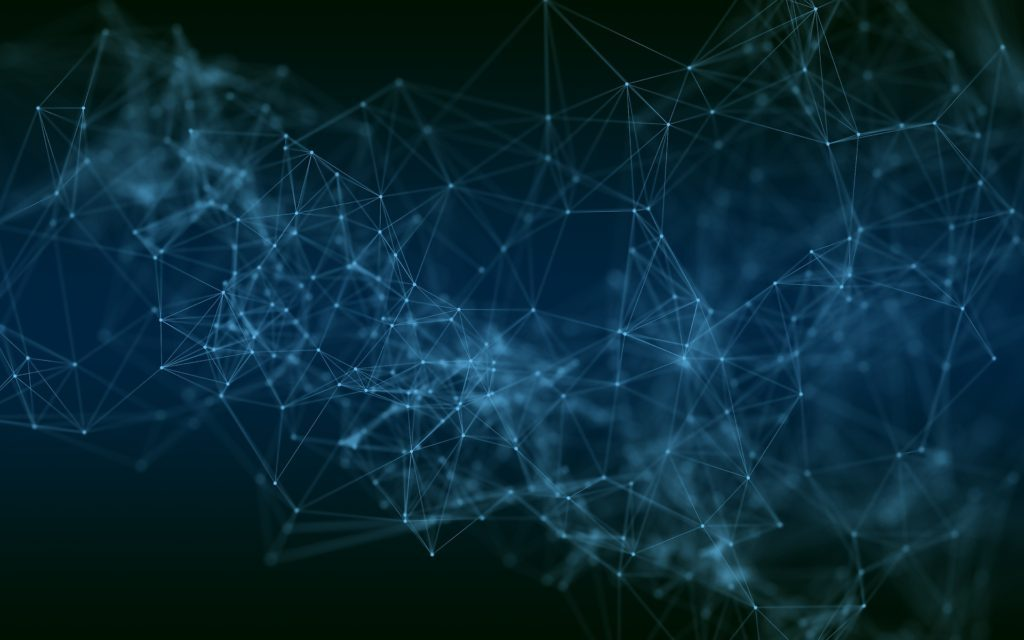
\includegraphics[
        width=\paperwidth,
        height=\paperheight
    ]{city-background.jpg}
};

% --------------------------------------------------
% Dark Overlay
% --------------------------------------------------

\fill[
    DarkBlue,
    opacity=0.48
]
(current page.south west)
rectangle
(current page.north east);

% --------------------------------------------------
% Main Title
% --------------------------------------------------

\node[
    text=TechYellow,
    align=center,
    font=\fontsize{30}{34}\selectfont\bfseries
]
at ([yshift=-2.45cm]current page.north)
{
    Edge Computing
};

% --------------------------------------------------
% Subtitle
% --------------------------------------------------

\node[
    text=White,
    align=center,
    font=\fontsize{20}{24}\selectfont\bfseries
]
at ([yshift=-3.55cm]current page.north)
{
    A Distributed Computing Paradigm for IoT
};

% --------------------------------------------------
% Tagline
% --------------------------------------------------

\node[
    text=White,
    align=center,
    font=\fontsize{11}{15}\selectfont
]
at ([yshift=-4.35cm]current page.north)
{
    Bringing Computation, Storage, and Networking Closer to Data Sources
};

% --------------------------------------------------
% Author Information
% --------------------------------------------------

\node[
    anchor=west,
    align=left,
    text=White,
    font=\fontsize{10.5}{14}\selectfont
]
at ([xshift=0.55cm,yshift=1.55cm]
    current page.south west)
{
    \textbf{Shone Sajan}\\[2pt]
    Department of Computer Science and Engineering\\
    Saintgits College of Engineering, Pathanmuttom, Kerala, India
};

\end{tikzpicture}

\end{frame}


% ==================================================
% SLIDE 01
% INTERNET OF THINGS
% ==================================================

\begin{frame}[plain]

\begin{tikzpicture}[remember picture,overlay]

% --------------------------------------------------
% Background
% --------------------------------------------------

\node[
    anchor=south west,
    inner sep=0pt
]
at (current page.south west)
{
    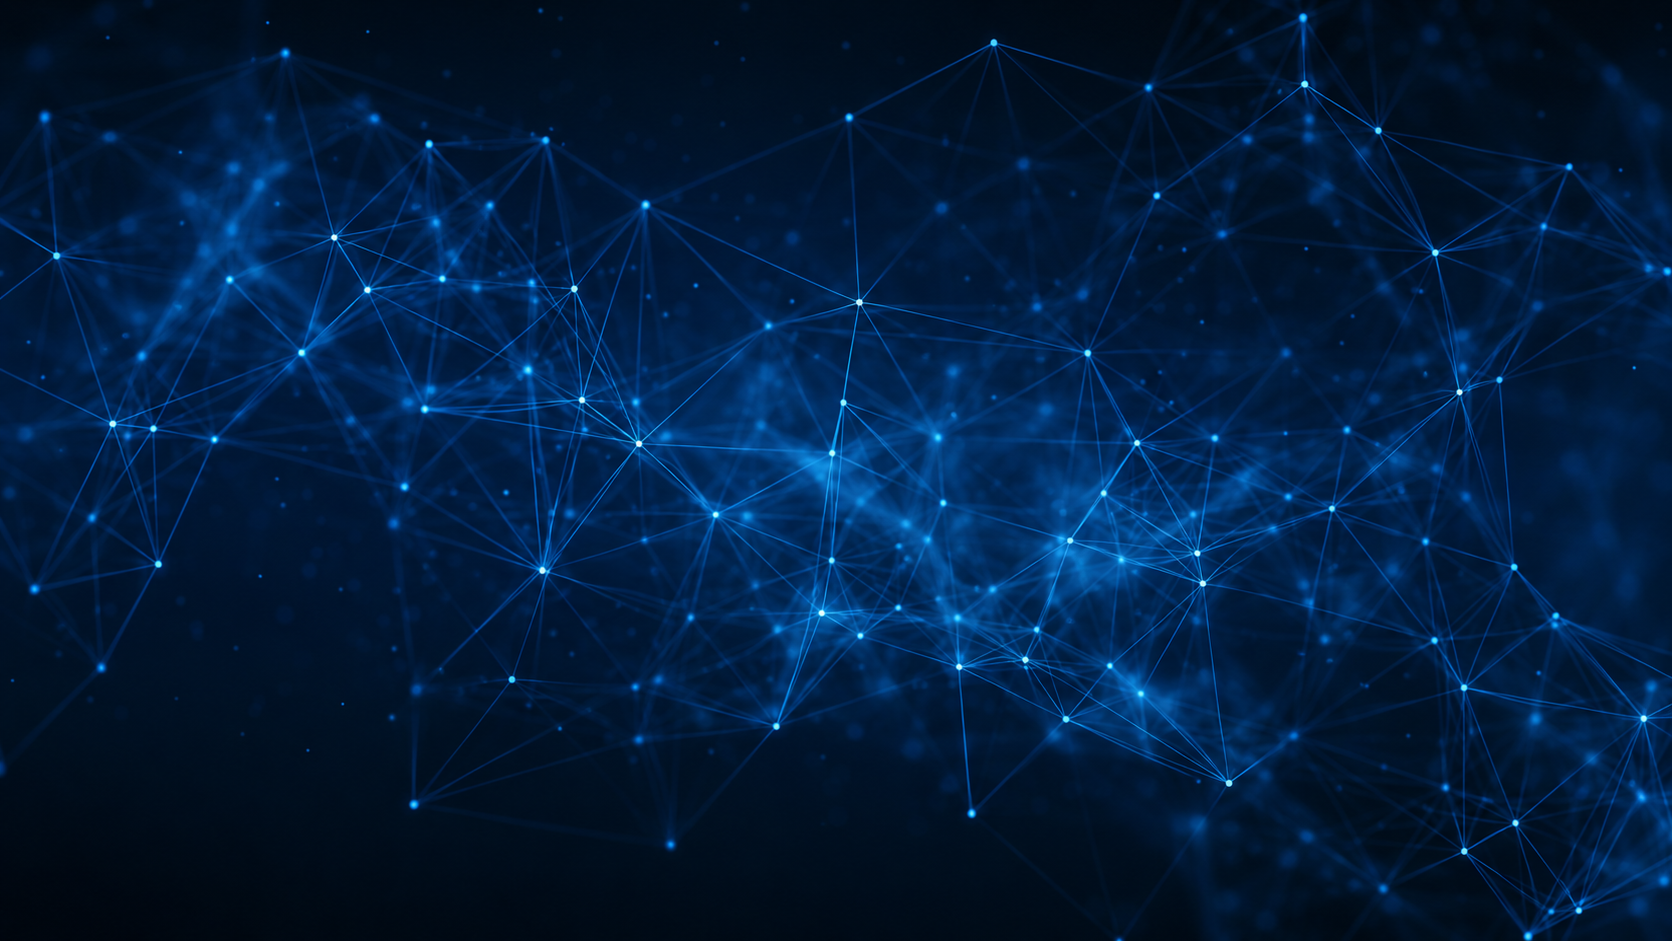
\includegraphics[
        width=\paperwidth,
        height=\paperheight
    ]{121.png}
};

% --------------------------------------------------
% Dark Overlay
% --------------------------------------------------

\fill[
    DarkBlue,
    opacity=0.72
]
(current page.south west)
rectangle
(current page.north east);

% --------------------------------------------------
% Slide Number
% --------------------------------------------------

\node[
    anchor=west,
    text=TechYellow,
    font=\fontsize{16}{18}\selectfont\bfseries
]
at ([xshift=0.8cm,yshift=-1.0cm]
    current page.north west)
{
    01
};

% --------------------------------------------------
% Slide Title
% --------------------------------------------------

\node[
    anchor=west,
    text=White,
    font=\fontsize{20}{24}\selectfont\bfseries
]
at ([xshift=2.0cm,yshift=-1.1cm]
    current page.north west)
{
    Internet of Things (IoT)
};

% --------------------------------------------------
% IoT Definition
% --------------------------------------------------

\node[
    anchor=north,
    text=SoftWhite,
    text width=11.5cm,
    align=justify,
    font=\fontsize{10.5}{14}\selectfont
]
at ([yshift=-1.60cm]current page.north)
{
    The Internet of Things (IoT) is a network of physical
    objects embedded with sensors, software, processing
    capabilities, and communication technologies that
    enable them to collect, exchange, and act upon data
    over a network with minimal human intervention.
};

% --------------------------------------------------
% Why Does the World Need IoT?
% --------------------------------------------------

\node[
    anchor=north west,
    text=TechYellow,
    font=\fontsize{11}{19}\selectfont\bfseries
]
at ([xshift=2.15cm,yshift=-3.65cm]
    current page.north west)
{
    Why does the world need IoT?
};

% --------------------------------------------------
% Explanation
% --------------------------------------------------

\node[
    anchor=north west,
    text=SoftWhite,
    text width=11.5cm,
    align=justify,
    font=\fontsize{10.5}{14}\selectfont
]
at ([xshift=2.15cm,yshift=-4.05cm]
    current page.north west)
{
    The number of connected devices and the amount of data
    generated by them are enormous. Instead of humans
    constantly checking everything manually,
    \textbf{IoT allows systems to observe the physical
    world continuously.}
};

% --------------------------------------------------
% Smart Home Example Box
% --------------------------------------------------

\node[
    anchor=north west,
    draw=TechCyan,
    line width=0.8pt,
    rounded corners=6pt,
    fill=BoxBlue,
    fill opacity=0.95,
    text opacity=1,
    text width=10.8cm,
    inner xsep=0.35cm,
    inner ysep=0.28cm
]
at ([xshift=2.15cm,yshift=-6.15cm]
    current page.north west)
{
    \textcolor{TechYellow}{
        \fontsize{13}{16}\selectfont\bfseries
        Smart Home Example
    }

    \par\vspace{0.12cm}

    \textcolor{SoftWhite}{
        \fontsize{10}{14}\selectfont
        A smart thermostat senses the room temperature,
        sends the data through a network, and automatically
        adjusts the air conditioning based on the user's
        settings.
    }
};

\end{tikzpicture}

\end{frame}


% ==================================================
% SLIDE 02
% IoT ARCHITECTURE
% ==================================================

\begin{frame}[plain]

\begin{tikzpicture}[remember picture,overlay]

% --------------------------------------------------
% Background
% --------------------------------------------------

\node[
    anchor=south west,
    inner sep=0pt
]
at (current page.south west)
{
    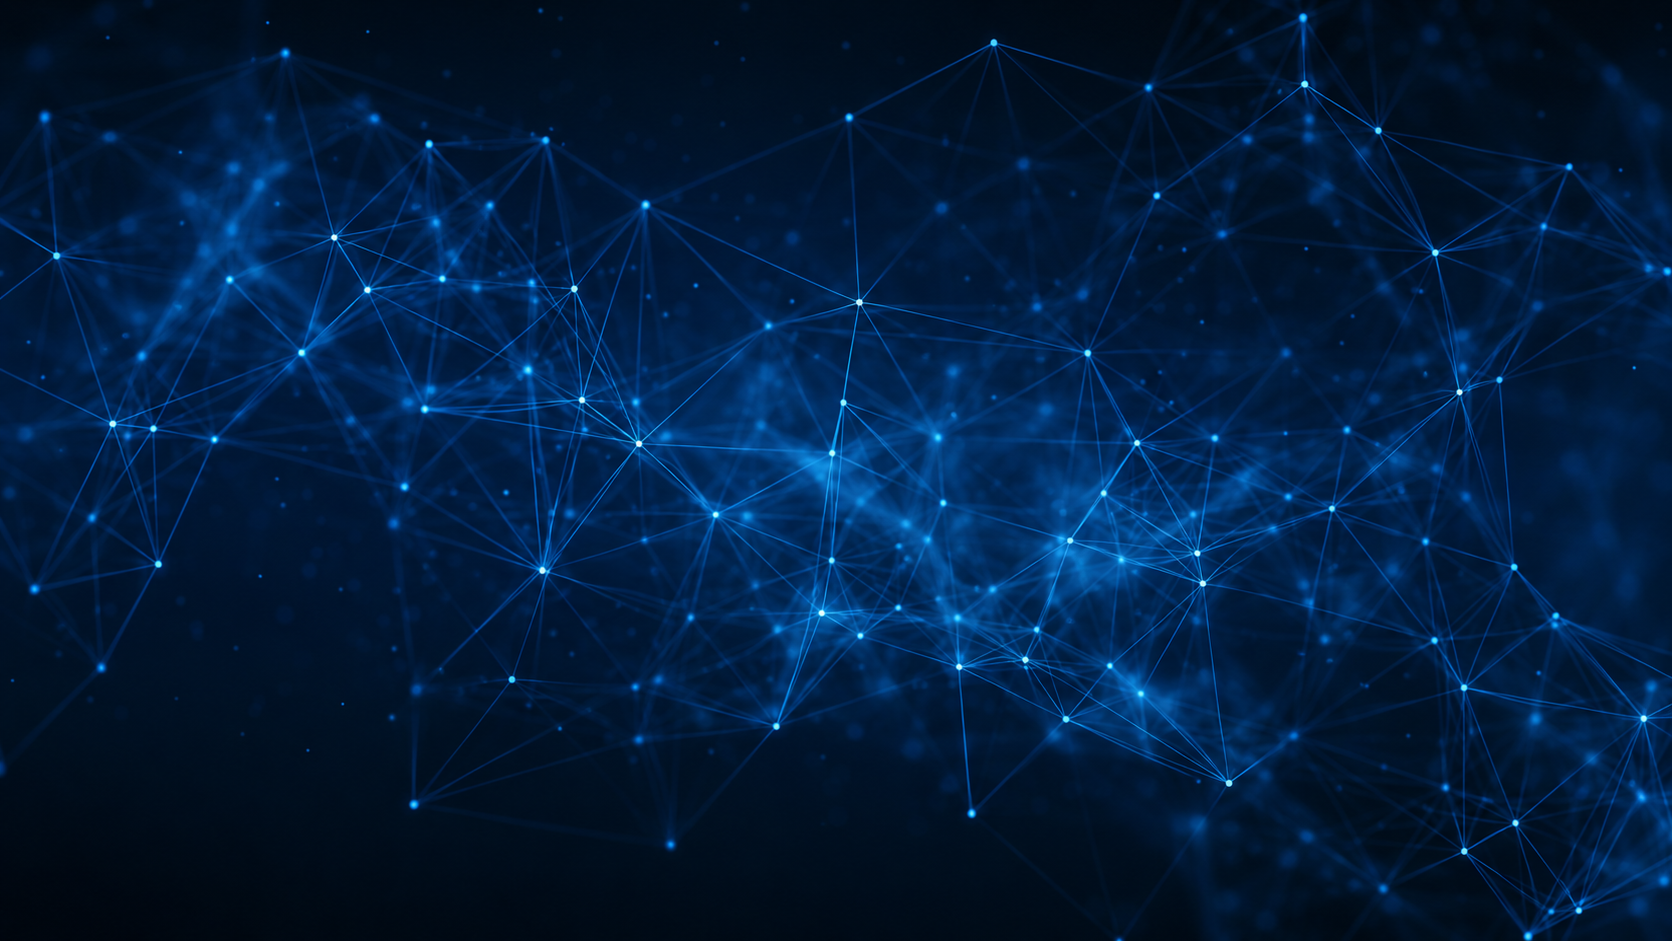
\includegraphics[
        width=\paperwidth,
        height=\paperheight
    ]{121.png}
};

% --------------------------------------------------
% Dark Overlay
% --------------------------------------------------

\fill[
    DarkBlue,
    opacity=0.72
]
(current page.south west)
rectangle
(current page.north east);

% --------------------------------------------------
% Slide Number
% --------------------------------------------------

\node[
    anchor=west,
    text=TechYellow,
    font=\fontsize{16}{18}\selectfont\bfseries
]
at ([xshift=0.8cm,yshift=-1.0cm]
    current page.north west)
{
    02
};

% --------------------------------------------------
% Slide Title
% --------------------------------------------------

\node[
    anchor=west,
    text=White,
    font=\fontsize{18}{24}\selectfont\bfseries
]
at ([xshift=2.0cm,yshift=-1.0cm]
    current page.north west)
{
    IoT Architecture
};

% --------------------------------------------------
% Architecture Image
% --------------------------------------------------

\node[
    anchor=north,
    draw=TechCyan,
    fill=White,
    fill opacity=1,
    text opacity=1,
    line width=0.8pt,
    rounded corners=6pt,
    inner sep=0.12cm
]
at ([yshift=-1.55cm]current page.north)
{
    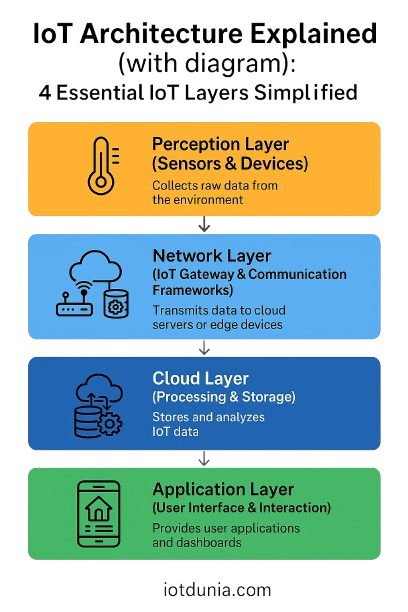
\includegraphics[
        width=12.0cm,
        height=6.75cm,
        keepaspectratio
    ]{iot-architecture.png}
};

% --------------------------------------------------
% Caption
% --------------------------------------------------

\node[
    anchor=north,
    text=SoftWhite,
    text width=11.5cm,
    align=center,
    font=\fontsize{8.5}{11}\selectfont
]
at ([yshift=-8.55cm]current page.north)
{

};

\end{tikzpicture}

\end{frame}


% ==================================================
% END
% ==================================================
% % ==================================================
% SLIDE 04
% CHALLENGES OF IoT
% ==================================================

\begin{frame}[plain]

\begin{tikzpicture}[remember picture,overlay]

% --------------------------------------------------
% Background
% --------------------------------------------------

\node[
    anchor=south west,
    inner sep=0pt
]
at (current page.south west)
{
    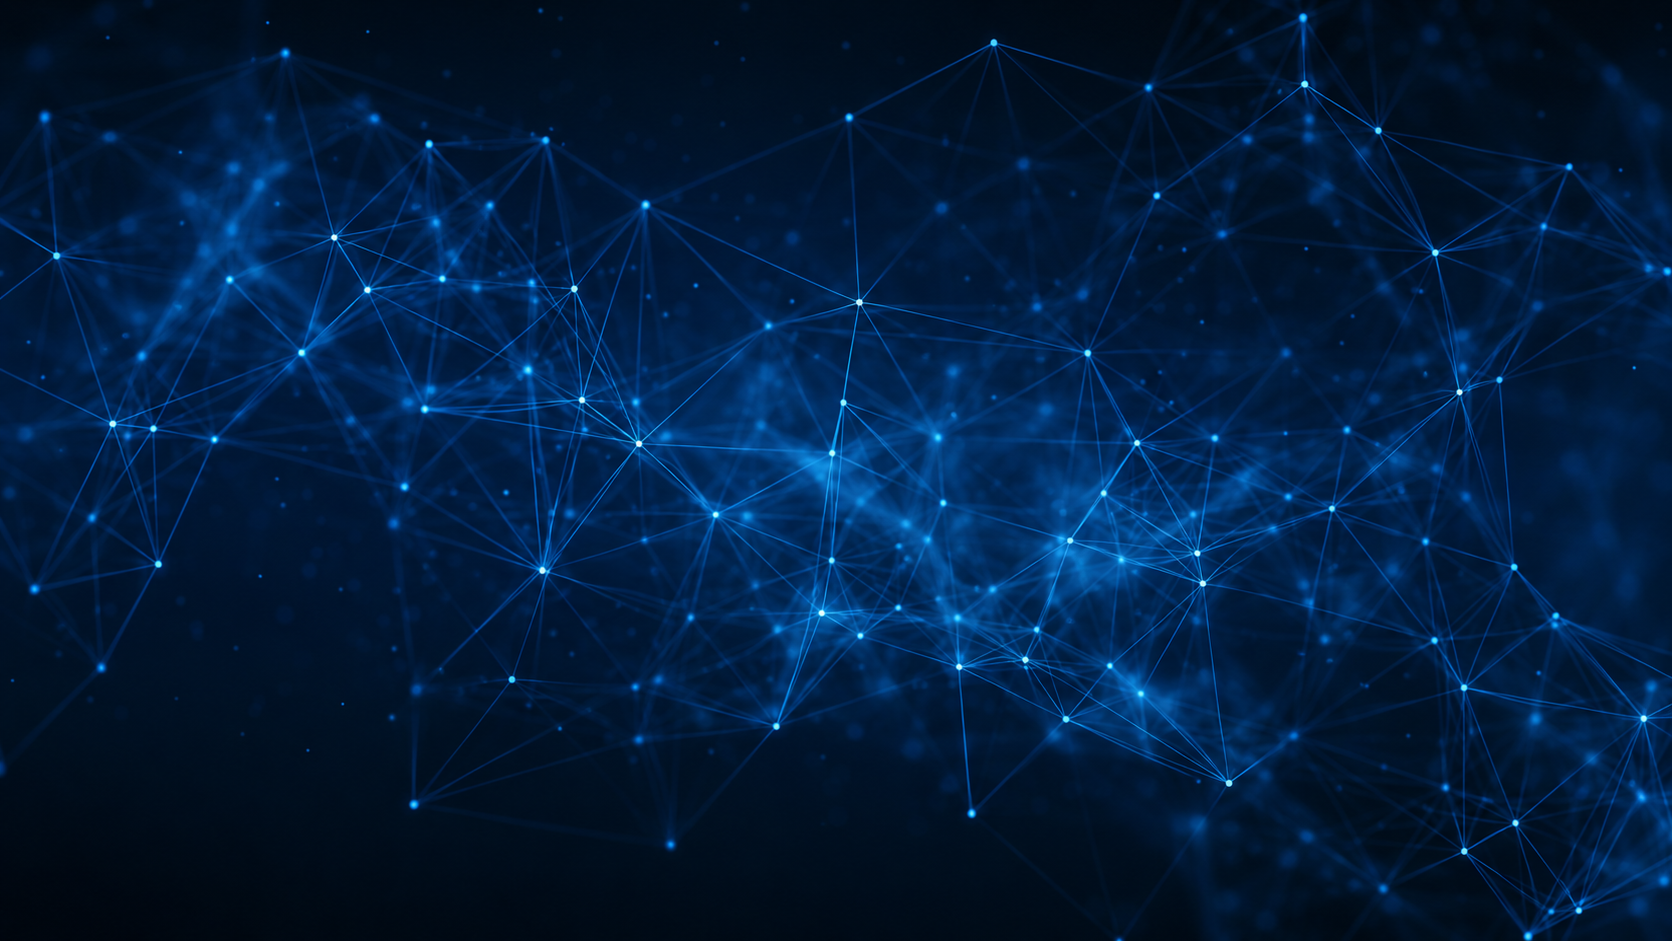
\includegraphics[
        width=\paperwidth,
        height=\paperheight
    ]{121.png}
};

% --------------------------------------------------
% Dark Overlay
% --------------------------------------------------

\fill[
    DarkBlue,
    opacity=0.72
]
(current page.south west)
rectangle
(current page.north east);

% --------------------------------------------------
% Slide Number
% --------------------------------------------------

\node[
    anchor=west,
    text=TechYellow,
    font=\fontsize{14}{16}\selectfont\bfseries
]
at ([xshift=0.8cm,yshift=-0.75cm]
    current page.north west)
{
    04
};

% --------------------------------------------------
% Slide Title
% --------------------------------------------------

\node[
    anchor=west,
    text=White,
    font=\fontsize{18}{22}\selectfont\bfseries
]
at ([xshift=1.8cm,yshift=-0.75cm]
    current page.north west)
{
    Challenges of IoT
};

% --------------------------------------------------
% Introductory Text
% --------------------------------------------------

\node[
    anchor=north,
    text=SoftWhite,
    text width=14.0cm,
    align=center,
    font=\fontsize{8.5}{11}\selectfont
]
at ([yshift=-1.25cm]current page.north)
{
    As IoT systems continue to grow, several challenges
    affect their security, scalability, reliability, and performance.
};


% ==================================================
% ROW 1
% ==================================================

% --------------------------------------------------
% Challenge 01
% --------------------------------------------------

\node[
    anchor=north west,
    draw=TechCyan,
    line width=0.7pt,
    rounded corners=5pt,
    fill=BoxTeal,
    text width=6.4cm,
    minimum height=1.65cm,
    inner xsep=0.28cm,
    inner ysep=0.18cm
]
at ([xshift=0.8cm,yshift=-1.95cm]
    current page.north west)
{
    \textcolor{TechYellow}{
        \fontsize{10}{12}\selectfont\bfseries
        01 \quad Security
    }

    \par\vspace{0.04cm}

    \textcolor{SoftWhite}{
        \fontsize{8}{10.5}\selectfont
        Connected devices increase the risk of
        cyberattacks, unauthorized access, and data breaches.
    }
};


% --------------------------------------------------
% Challenge 02
% --------------------------------------------------

\node[
    anchor=north west,
    draw=TechYellow,
    line width=0.7pt,
    rounded corners=5pt,
    fill=BoxPurple,
    text width=6.4cm,
    minimum height=1.65cm,
    inner xsep=0.28cm,
    inner ysep=0.18cm
]
at ([xshift=8.2cm,yshift=-1.95cm]
    current page.north west)
{
    \textcolor{TechYellow}{
        \fontsize{10}{12}\selectfont\bfseries
        02 \quad Data Privacy
    }

    \par\vspace{0.04cm}

    \textcolor{SoftWhite}{
        \fontsize{8}{10.5}\selectfont
        Continuous data collection creates concerns
        about privacy, ownership, and misuse.
    }
};


% ==================================================
% ROW 2
% ==================================================

% --------------------------------------------------
% Challenge 03
% --------------------------------------------------

\node[
    anchor=north west,
    draw=TechCyan,
    line width=0.7pt,
    rounded corners=5pt,
    fill=BoxIndigo,
    text width=6.4cm,
    minimum height=1.65cm,
    inner xsep=0.28cm,
    inner ysep=0.18cm
]
at ([xshift=0.8cm,yshift=-4.15cm]
    current page.north west)
{
    \textcolor{TechYellow}{
        \fontsize{10}{12}\selectfont\bfseries
        03 \quad Scalability
    }

    \par\vspace{0.04cm}

    \textcolor{SoftWhite}{
        \fontsize{8}{10.5}\selectfont
        Supporting billions of devices requires
        scalable infrastructure and resource management.
    }
};


% --------------------------------------------------
% Challenge 04
% --------------------------------------------------

\node[
    anchor=north west,
    draw=TechYellow,
    line width=0.7pt,
    rounded corners=5pt,
    fill=BoxEmerald,
    text width=6.4cm,
    minimum height=1.65cm,
    inner xsep=0.28cm,
    inner ysep=0.18cm
]
at ([xshift=8.2cm,yshift=-4.15cm]
    current page.north west)
{
    \textcolor{TechYellow}{
        \fontsize{10}{12}\selectfont\bfseries
        04 \quad Connectivity
    }

    \par\vspace{0.04cm}

    \textcolor{SoftWhite}{
        \fontsize{8}{10.5}\selectfont
        Unstable networks, limited bandwidth, and
        intermittent connectivity affect IoT performance.
    }
};


% ==================================================
% ROW 3
% ==================================================

% --------------------------------------------------
% Challenge 05
% --------------------------------------------------

\node[
    anchor=north west,
    draw=TechCyan,
    line width=0.7pt,
    rounded corners=5pt,
    fill=BoxWine,
    text width=6.4cm,
    minimum height=1.65cm,
    inner xsep=0.28cm,
    inner ysep=0.18cm
]
at ([xshift=0.8cm,yshift=-6.35cm]
    current page.north west)
{
    \textcolor{TechYellow}{
        \fontsize{10}{12}\selectfont\bfseries
        05 \quad Data Processing
    }

    \par\vspace{0.04cm}

    \textcolor{SoftWhite}{
        \fontsize{8}{10.5}\selectfont
        Massive IoT data creates significant processing
        and storage requirements.
    }
};


% --------------------------------------------------
% Challenge 06
% --------------------------------------------------

\node[
    anchor=north west,
    draw=TechYellow,
    line width=0.7pt,
    rounded corners=5pt,
    fill=BoxSlate,
    text width=6.4cm,
    minimum height=1.65cm,
    inner xsep=0.28cm,
    inner ysep=0.18cm
]
at ([xshift=8.2cm,yshift=-6.35cm]
    current page.north west)
{
    \textcolor{TechYellow}{
        \fontsize{10}{12}\selectfont\bfseries
        06 \quad Energy Constraints
    }

    \par\vspace{0.04cm}

    \textcolor{SoftWhite}{
        \fontsize{8}{10.5}\selectfont
        Battery-powered devices require energy-efficient
        communication and computation.
    }
};

\end{tikzpicture}

\end{frame}


% ==================================================
% SLIDE 05
% IOT IS CREATING A DATA PROBLEM
% ==================================================

\begin{frame}[plain]

\begin{tikzpicture}[remember picture,overlay]

% --------------------------------------------------
% Background
% --------------------------------------------------

\node[
    anchor=south west,
    inner sep=0pt
]
at (current page.south west)
{
    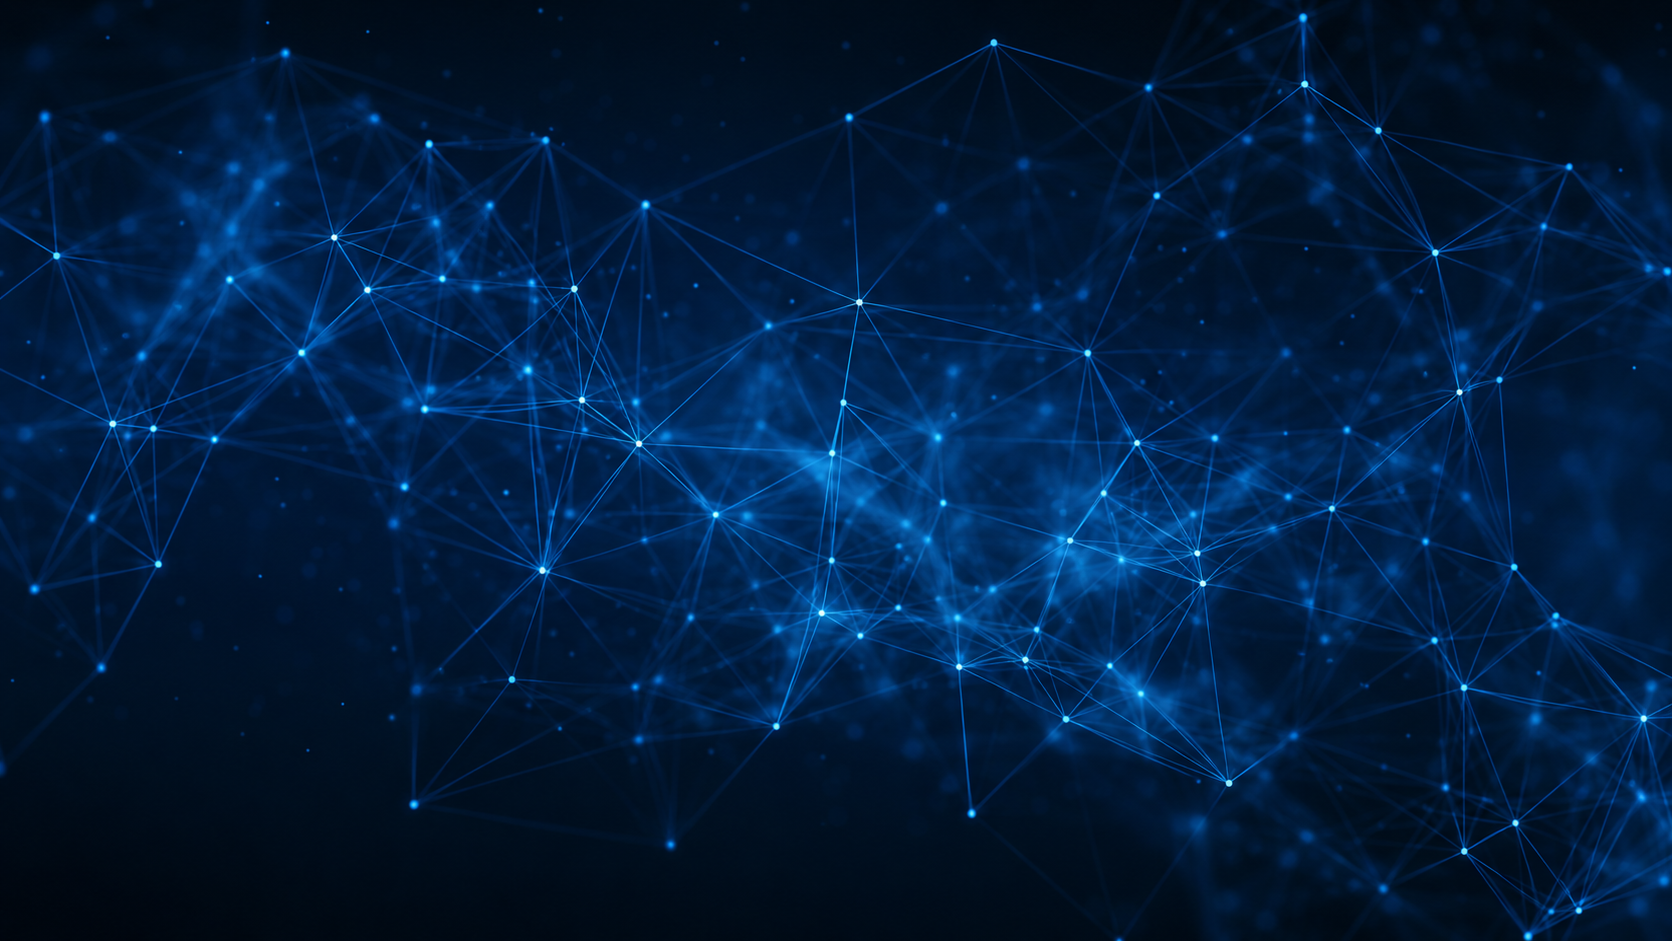
\includegraphics[
        width=\paperwidth,
        height=\paperheight
    ]{121.png}
};

% --------------------------------------------------
% Dark Overlay
% --------------------------------------------------

\fill[
    DarkBlue,
    opacity=0.72
]
(current page.south west)
rectangle
(current page.north east);

% --------------------------------------------------
% Slide Number
% --------------------------------------------------

\node[
    anchor=west,
    text=TechYellow,
    font=\fontsize{14}{16}\selectfont\bfseries
]
at ([xshift=0.8cm,yshift=-0.65cm]
    current page.north west)
{
    05
};

% --------------------------------------------------
% Slide Title
% --------------------------------------------------

\node[
    anchor=west,
    text=White,
    font=\fontsize{18}{22}\selectfont\bfseries
]
at ([xshift=1.8cm,yshift=-0.65cm]
    current page.north west)
{
    IoT Is Creating a Data Problem
};

% --------------------------------------------------
% Left Column: Large Prominent Pipeline Diagram
% --------------------------------------------------

\node[
    anchor=north west,
    draw=TechCyan,
    fill=White,
    fill opacity=1,
    text opacity=1,
    line width=0.8pt,
    rounded corners=6pt,
    inner sep=0.12cm
]
at ([xshift=0.8cm,yshift=-1.30cm]
    current page.north west)
{
    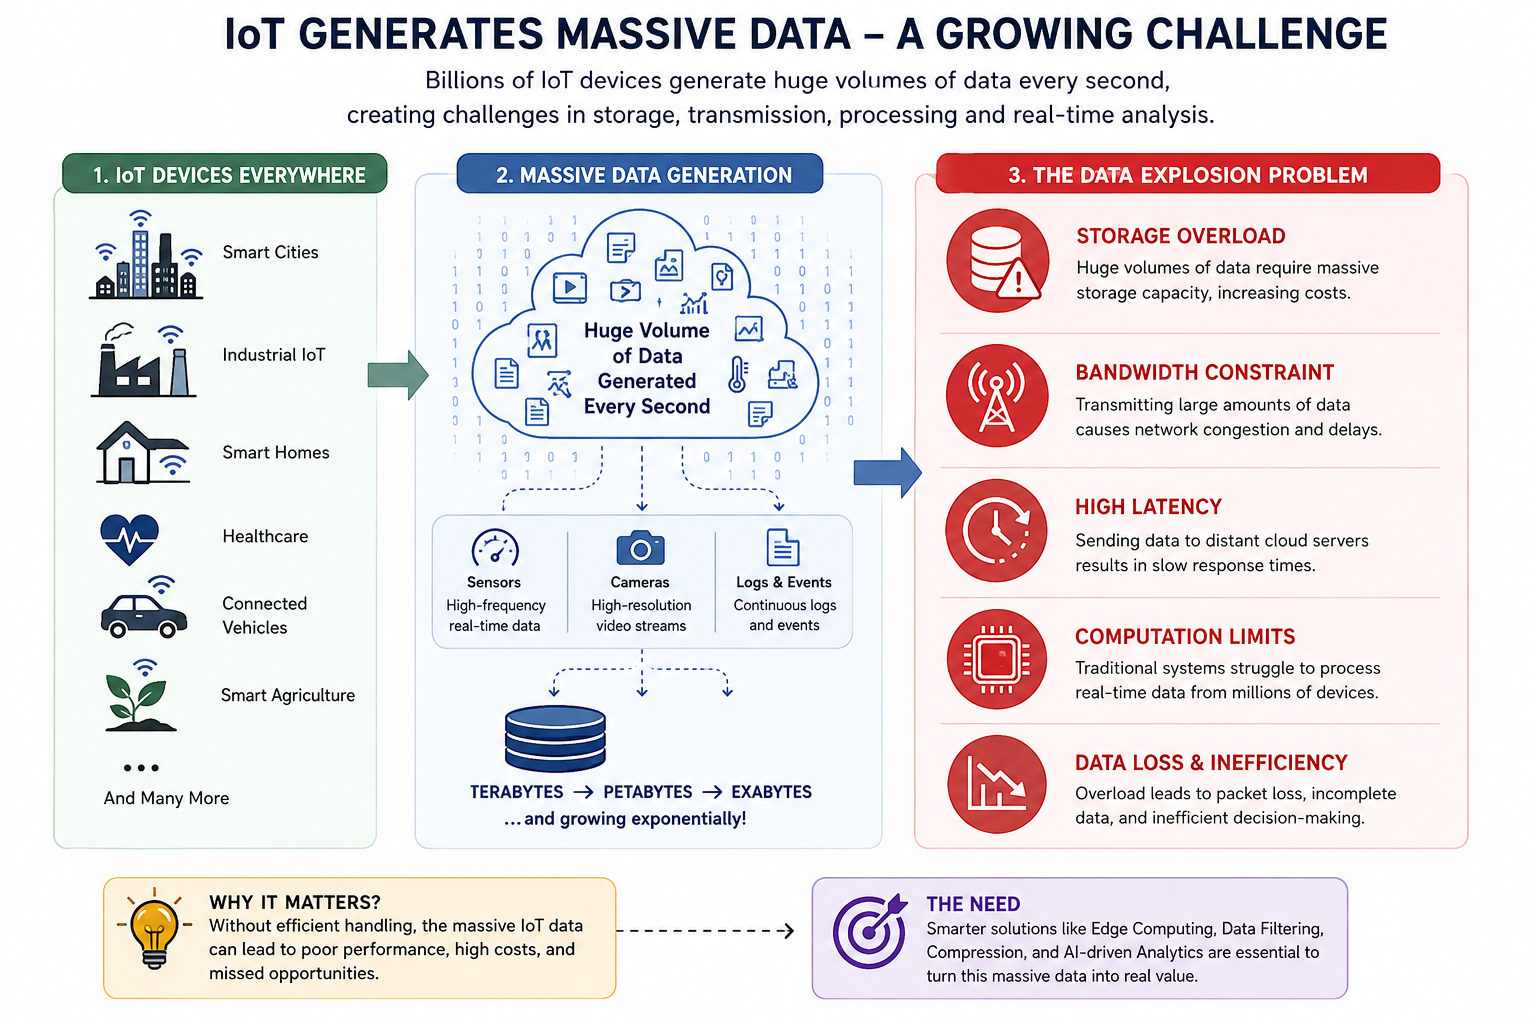
\includegraphics[
        width=6.6cm,
        height=5.7cm,
        keepaspectratio
    ]{iot_data_pic.png}
};


% --------------------------------------------------
% Right Column: 3 Well-Spaced Problem Cards
% --------------------------------------------------

% Problem 1: Latency
\node[
    anchor=north west,
    draw=TechYellow,
    line width=0.7pt,
    rounded corners=6pt,
    fill=BoxBlue,
    fill opacity=0.95,
    text opacity=1,
    text width=6.6cm,
    minimum height=1.65cm,
    inner xsep=0.25cm,
    inner ysep=0.16cm
]
at ([xshift=8.2cm,yshift=-1.30cm]
    current page.north west)
{
    \textcolor{TechYellow}{
        \fontsize{10}{12}\selectfont\bfseries
        01 \quad LATENCY
    }

    \par\vspace{0.04cm}

    \textcolor{SoftWhite}{
        \fontsize{8.5}{11.5}\selectfont
        Slow response for time-critical applications.
    }
};

% Problem 2: Bandwidth
\node[
    anchor=north west,
    draw=TechCyan,
    line width=0.7pt,
    rounded corners=6pt,
    fill=BoxBlue,
    fill opacity=0.95,
    text opacity=1,
    text width=6.6cm,
    minimum height=1.65cm,
    inner xsep=0.25cm,
    inner ysep=0.16cm
]
at ([xshift=8.2cm,yshift=-3.25cm]
    current page.north west)
{
    \textcolor{TechCyan}{
        \fontsize{10}{12}\selectfont\bfseries
        02 \quad BANDWIDTH
    }

    \par\vspace{0.04cm}

    \textcolor{SoftWhite}{
        \fontsize{8.5}{11.5}\selectfont
        Large volumes of data must be transmitted.
    }
};

% Problem 3: Computation
\node[
    anchor=north west,
    draw=TechYellow,
    line width=0.7pt,
    rounded corners=6pt,
    fill=BoxBlue,
    fill opacity=0.95,
    text opacity=1,
    text width=6.6cm,
    minimum height=1.65cm,
    inner xsep=0.25cm,
    inner ysep=0.16cm
]
at ([xshift=8.2cm,yshift=-5.20cm]
    current page.north west)
{
    \textcolor{TechYellow}{
        \fontsize{10}{12}\selectfont\bfseries
        03 \quad COMPUTATION
    }

    \par\vspace{0.04cm}

    \textcolor{SoftWhite}{
        \fontsize{8.5}{11.5}\selectfont
        IoT devices have limited processing resources.
    }
};


% --------------------------------------------------
% Bottom Key Message Banner (At Very Bottom)
% --------------------------------------------------

\node[
    anchor=north west,
    draw=TechCyan,
    line width=0.8pt,
    rounded corners=6pt,
    fill=DarkBlue,
    fill opacity=0.95,
    text opacity=1,
    text width=14.0cm,
    align=center,
    inner xsep=0.25cm,
    inner ysep=0.18cm
]
at ([xshift=0.8cm,yshift=-7.60cm]
    current page.north west)
{
    \textcolor{TechYellow}{\fontsize{9.5}{12}\selectfont\bfseries Key Message:}\;\;
    \textcolor{White}{\fontsize{9.5}{12}\selectfont The challenge is no longer just collecting data --- it is \textbf{processing it fast enough}.}
};

\end{tikzpicture}

\end{frame}


% ==================================================
% SLIDE 06
% INTRODUCTION TO EDGE COMPUTING
% ==================================================

\begin{frame}[plain]

\begin{tikzpicture}[remember picture,overlay]

% --------------------------------------------------
% Background
% --------------------------------------------------

\node[
    anchor=south west,
    inner sep=0pt
]
at (current page.south west)
{
    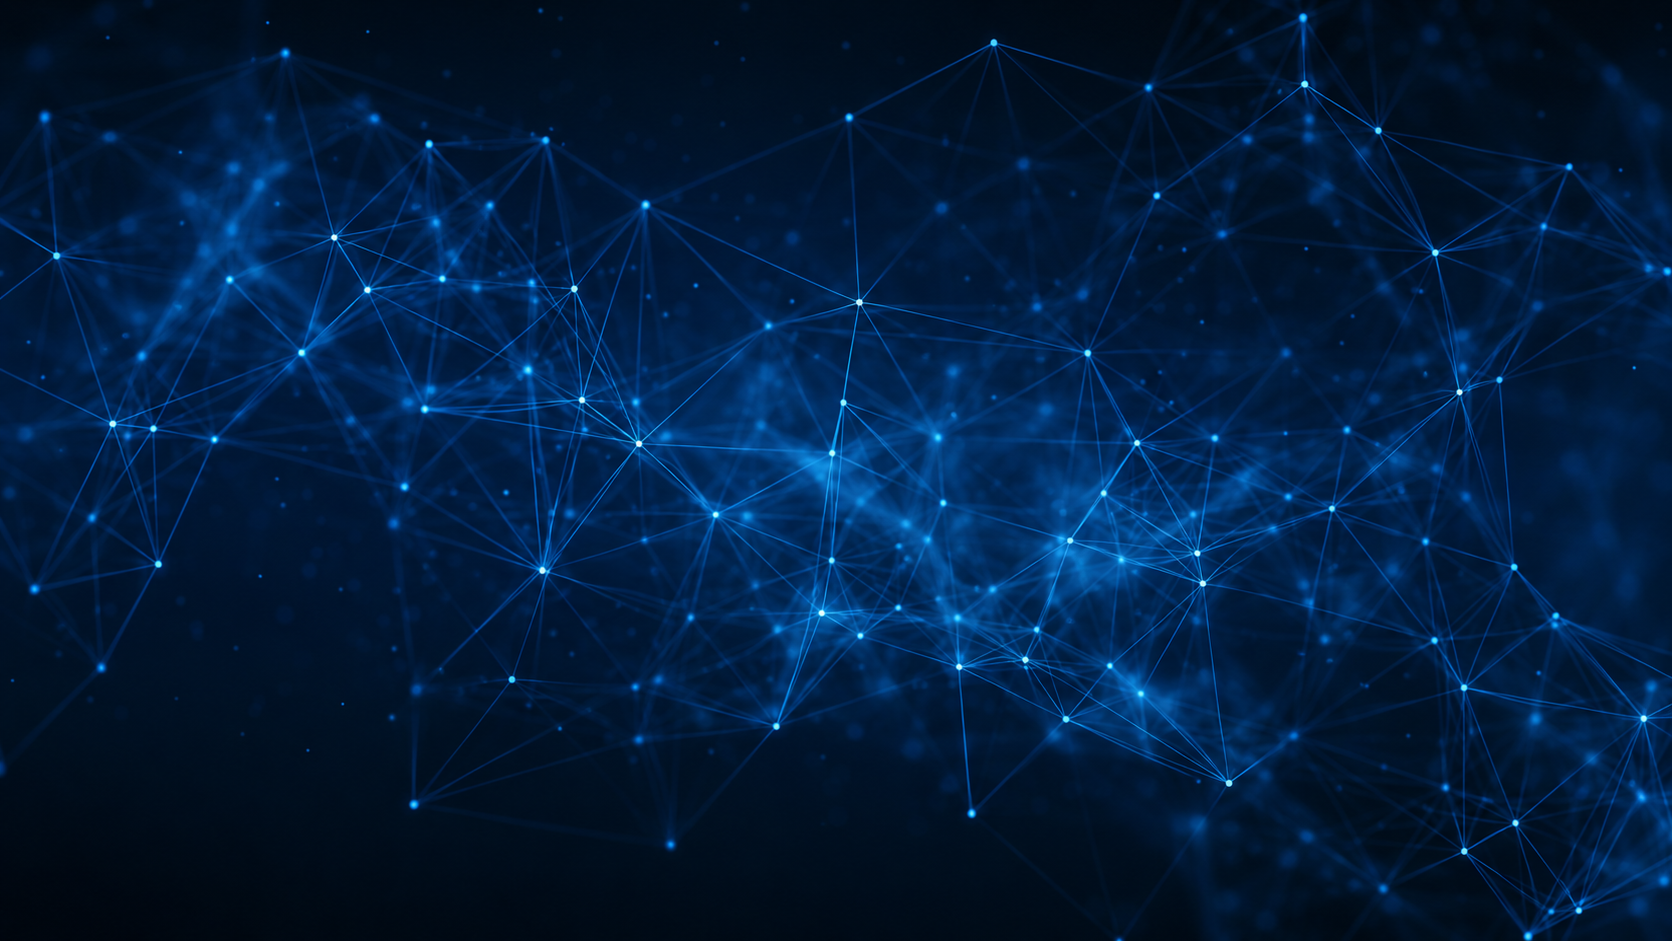
\includegraphics[
        width=\paperwidth,
        height=\paperheight
    ]{121.png}
};

% --------------------------------------------------
% Dark Overlay
% --------------------------------------------------

\fill[
    DarkBlue,
    opacity=0.72
]
(current page.south west)
rectangle
(current page.north east);

% --------------------------------------------------
% Slide Number
% --------------------------------------------------

\node[
    anchor=west,
    text=TechYellow,
    font=\fontsize{14}{16}\selectfont\bfseries
]
at ([xshift=0.8cm,yshift=-0.65cm]
    current page.north west)
{
    06
};

% --------------------------------------------------
% Slide Title
% --------------------------------------------------

\node[
    anchor=west,
    text=White,
    font=\fontsize{18}{22}\selectfont\bfseries
]
at ([xshift=1.8cm,yshift=-0.65cm]
    current page.north west)
{
    Introduction to Edge Computing
};

% --------------------------------------------------
% Definition (No Box, Clean Text)
% --------------------------------------------------

\node[
    anchor=north west,
    text width=14.2cm,
    align=justify,
    inner sep=0pt
]
at ([xshift=0.8cm,yshift=-1.15cm]
    current page.north west)
{
    \textcolor{TechYellow}{\fontsize{11}{14}\selectfont\bfseries Definition}\\[3pt]
    \textcolor{SoftWhite}{\fontsize{9.5}{13.5}\selectfont
    Edge Computing is a distributed computing paradigm that brings computation and data storage closer to the devices and locations where data is generated. [1]}
};

% --------------------------------------------------
% Basic Architecture Section
% --------------------------------------------------

\node[
    anchor=north west,
    text width=14.2cm,
    inner sep=0pt
]
at ([xshift=0.8cm,yshift=-2.85cm]
    current page.north west)
{
    \textcolor{TechYellow}{\fontsize{11}{14}\selectfont\bfseries Basic Architecture}\\[4pt]
    \textcolor{White}{\fontsize{9.5}{13.5}\selectfont\bfseries IoT Devices $\;\rightarrow\;$ Edge Layer $\;\rightarrow\;$ Cloud}\\[4pt]
    \textcolor{TechCyan}{$\bullet$}\;\;\textcolor{White}{\fontsize{9}{12}\selectfont\bfseries IoT Devices:} \textcolor{SoftWhite}{\fontsize{9}{12}\selectfont Generate and collect data}\\[3pt]
    \textcolor{TechCyan}{$\bullet$}\;\;\textcolor{White}{\fontsize{9}{12}\selectfont\bfseries Edge Layer:} \textcolor{SoftWhite}{\fontsize{9}{12}\selectfont Performs processing closer to the data source}\\[3pt]
    \textcolor{TechCyan}{$\bullet$}\;\;\textcolor{White}{\fontsize{9}{12}\selectfont\bfseries Cloud:} \textcolor{SoftWhite}{\fontsize{9}{12}\selectfont Provides large-scale computation and storage}
};

% --------------------------------------------------
% Key Characteristics Section (Bulleted List)
% --------------------------------------------------

\node[
    anchor=north west,
    text width=14.2cm,
    inner sep=0pt
]
at ([xshift=0.8cm,yshift=-5.75cm]
    current page.north west)
{
    \textcolor{TechYellow}{\fontsize{11}{14}\selectfont\bfseries Key Characteristics}\\[4pt]
    \textcolor{TechCyan}{$\bullet$}\;\;\textcolor{White}{\fontsize{9}{12}\selectfont\bfseries Low Latency:} \textcolor{SoftWhite}{\fontsize{9}{12}\selectfont Enables faster response to time-sensitive applications}\\[3.5pt]
    \textcolor{TechCyan}{$\bullet$}\;\;\textcolor{White}{\fontsize{9}{12}\selectfont\bfseries Reduced Bandwidth Usage:} \textcolor{SoftWhite}{\fontsize{9}{12}\selectfont Minimizes the amount of data transferred to the cloud}\\[3.5pt]
    \textcolor{TechCyan}{$\bullet$}\;\;\textcolor{White}{\fontsize{9}{12}\selectfont\bfseries Real-Time Processing:} \textcolor{SoftWhite}{\fontsize{9}{12}\selectfont Enables decisions closer to the data source}\\[3.5pt]
    \textcolor{TechCyan}{$\bullet$}\;\;\textcolor{White}{\fontsize{9}{12}\selectfont\bfseries Distributed Computing:} \textcolor{SoftWhite}{\fontsize{9}{12}\selectfont Distributes computational workloads across edge and cloud resources}
};

\end{tikzpicture}

\end{frame}


% ==================================================
% SLIDE 07
% IoT--EDGE COMPUTING RELATIONSHIP
% ==================================================

\begin{frame}[plain]

\begin{tikzpicture}[remember picture,overlay]

% --------------------------------------------------
% Background
% --------------------------------------------------

\node[
    anchor=south west,
    inner sep=0pt
]
at (current page.south west)
{
    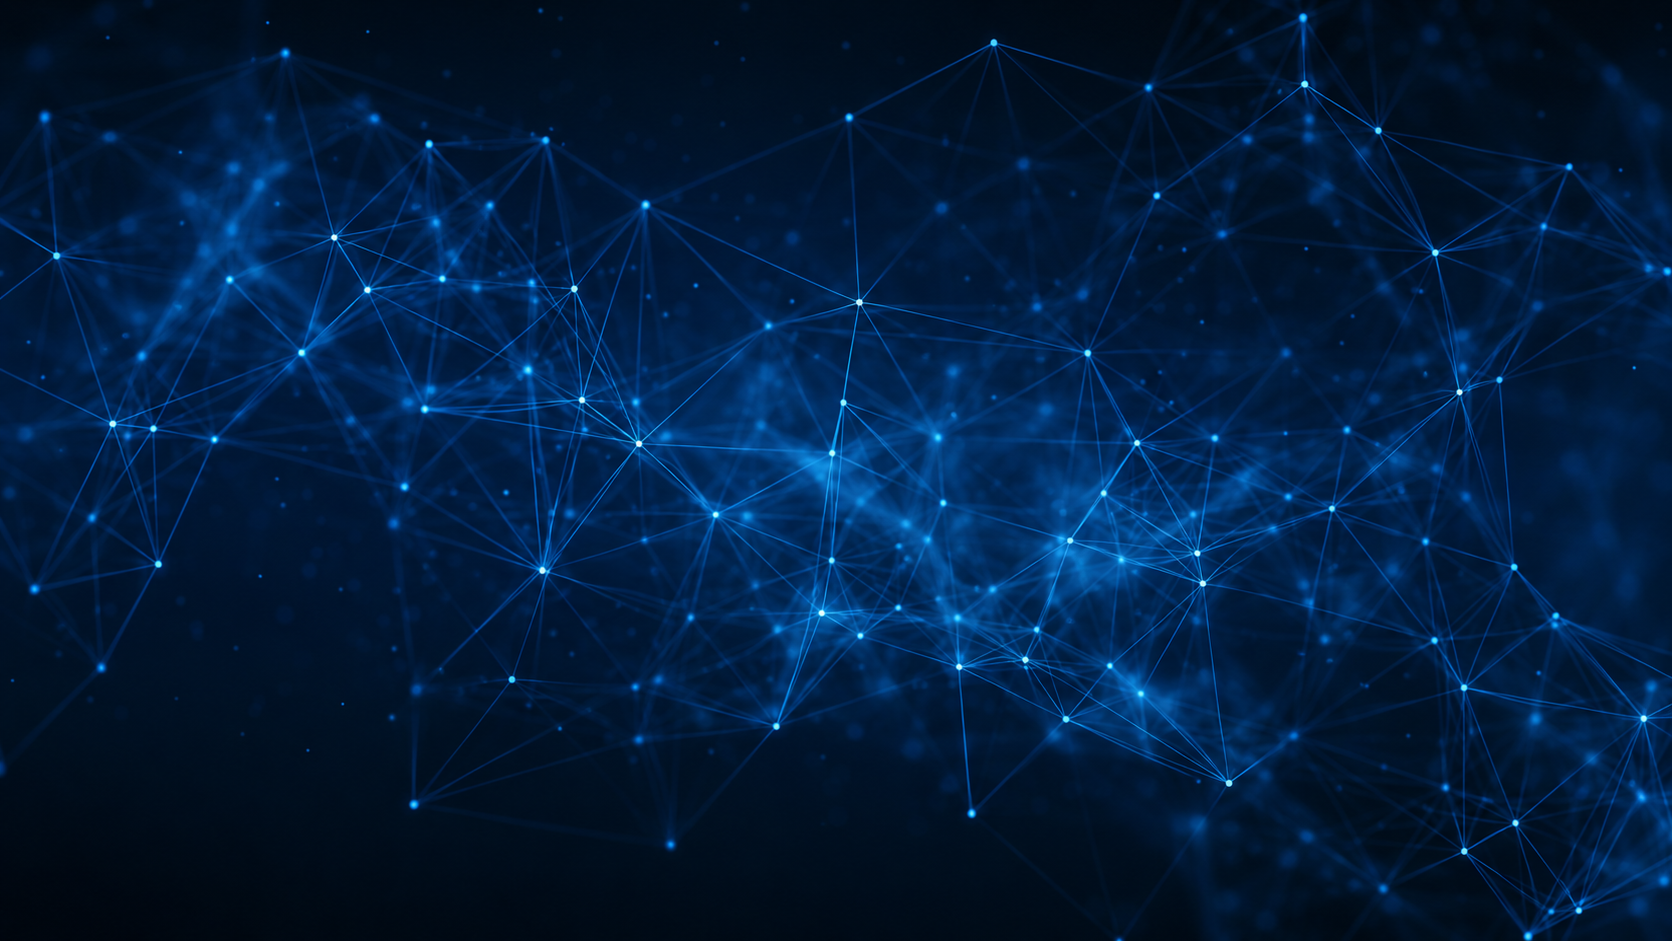
\includegraphics[
        width=\paperwidth,
        height=\paperheight
    ]{121.png}
};

% --------------------------------------------------
% Dark Overlay
% --------------------------------------------------

\fill[
    DarkBlue,
    opacity=0.72
]
(current page.south west)
rectangle
(current page.north east);

% --------------------------------------------------
% Slide Number
% --------------------------------------------------

\node[
    anchor=west,
    text=TechYellow,
    font=\fontsize{14}{16}\selectfont\bfseries
]
at ([xshift=0.8cm,yshift=-0.65cm]
    current page.north west)
{
    07
};

% --------------------------------------------------
% Slide Title
% --------------------------------------------------

\node[
    anchor=west,
    text=White,
    font=\fontsize{18}{22}\selectfont\bfseries
]
at ([xshift=1.8cm,yshift=-0.65cm]
    current page.north west)
{
    IoT--Edge Computing Relationship
};

% --------------------------------------------------
% Left Box: The IoT Data Bottleneck
% --------------------------------------------------

\node[
    anchor=north west,
    draw=TechYellow,
    line width=0.8pt,
    rounded corners=6pt,
    fill=BoxBlue,
    fill opacity=0.95,
    text opacity=1,
    text width=6.5cm,
    minimum height=5.60cm,
    inner xsep=0.28cm,
    inner ysep=0.22cm
]
at ([xshift=0.8cm,yshift=-1.20cm]
    current page.north west)
{
    \textcolor{TechYellow}{\fontsize{11}{13}\selectfont\bfseries The IoT Data Bottleneck}\\[8pt]
    \textcolor{TechCyan}{$\bullet$}\;\;\textcolor{White}{\fontsize{9}{12}\selectfont\bfseries Data Explosion:}\\[2pt]
    \hspace*{0.30cm}\textcolor{SoftWhite}{\fontsize{8.5}{11.5}\selectfont Continuous streams from sensors, cameras, machines \& vehicles.}\\[9pt]
    \textcolor{TechCyan}{$\bullet$}\;\;\textcolor{White}{\fontsize{9}{12}\selectfont\bfseries Device Constraints:}\\[2pt]
    \hspace*{0.30cm}\textcolor{SoftWhite}{\fontsize{8.5}{11.5}\selectfont Limited processing, storage, and energy resources.}\\[9pt]
    \textcolor{TechCyan}{$\bullet$}\;\;\textcolor{White}{\fontsize{9}{12}\selectfont\bfseries Cloud Overhead:}\\[2pt]
    \hspace*{0.30cm}\textcolor{SoftWhite}{\fontsize{8.5}{11.5}\selectfont Offloading all data causes high latency \& network congestion.}
};

% --------------------------------------------------
% Right Box: How Edge Complements IoT
% --------------------------------------------------

\node[
    anchor=north west,
    draw=TechCyan,
    line width=0.8pt,
    rounded corners=6pt,
    fill=BoxBlue,
    fill opacity=0.95,
    text opacity=1,
    text width=6.5cm,
    minimum height=5.60cm,
    inner xsep=0.28cm,
    inner ysep=0.22cm
]
at ([xshift=8.1cm,yshift=-1.20cm]
    current page.north west)
{
    \textcolor{TechCyan}{\fontsize{11}{13}\selectfont\bfseries How Edge Complements IoT}\\[8pt]
    \textcolor{TechCyan}{$\bullet$}\;\;\textcolor{White}{\fontsize{9}{12}\selectfont\bfseries Proximity Processing:}\\[2pt]
    \hspace*{0.30cm}\textcolor{SoftWhite}{\fontsize{8.5}{11.5}\selectfont Computes data directly near local generation points.}\\[9pt]
    \textcolor{TechCyan}{$\bullet$}\;\;\textcolor{White}{\fontsize{9}{12}\selectfont\bfseries Intelligent Filtering:}\\[2pt]
    \hspace*{0.30cm}\textcolor{SoftWhite}{\fontsize{8.5}{11.5}\selectfont Filters \& aggregates data before cloud transmission.}\\[9pt]
    \textcolor{TechCyan}{$\bullet$}\;\;\textcolor{White}{\fontsize{9}{12}\selectfont\bfseries Low-Latency Autonomy:}\\[2pt]
    \hspace*{0.30cm}\textcolor{SoftWhite}{\fontsize{8.5}{11.5}\selectfont Enables real-time actions without full cloud reliance.}
};

% --------------------------------------------------
% Bottom Summary Card: Distributed Ecosystem (Pushed To Bottom)
% --------------------------------------------------

\node[
    anchor=north west,
    draw=TechCyan,
    line width=0.8pt,
    rounded corners=6pt,
    fill=DarkBlue,
    fill opacity=0.95,
    text opacity=1,
    text width=14.0cm,
    align=center,
    inner xsep=0.25cm,
    inner ysep=0.16cm
]
at ([xshift=0.8cm,yshift=-7.40cm]
    current page.north west)
{
    \textcolor{TechYellow}{\fontsize{9.5}{12}\selectfont\bfseries Key Takeaway:}\;\;
    \textcolor{White}{\fontsize{9}{12}\selectfont
    Edge Computing does not replace the Cloud --- it forms a distributed \textbf{IoT $\rightarrow$ Edge $\rightarrow$ Cloud} ecosystem where Edge manages instant local processing while Cloud handles large-scale analytics.
    }
};

\end{tikzpicture}

\end{frame}


% ==================================================
% SLIDE 08
% EDGE COMPUTING ARCHITECTURE
% ==================================================

\begin{frame}[plain]

\begin{tikzpicture}[remember picture,overlay]

% --------------------------------------------------
% Background
% --------------------------------------------------

\node[
    anchor=south west,
    inner sep=0pt
]
at (current page.south west)
{
    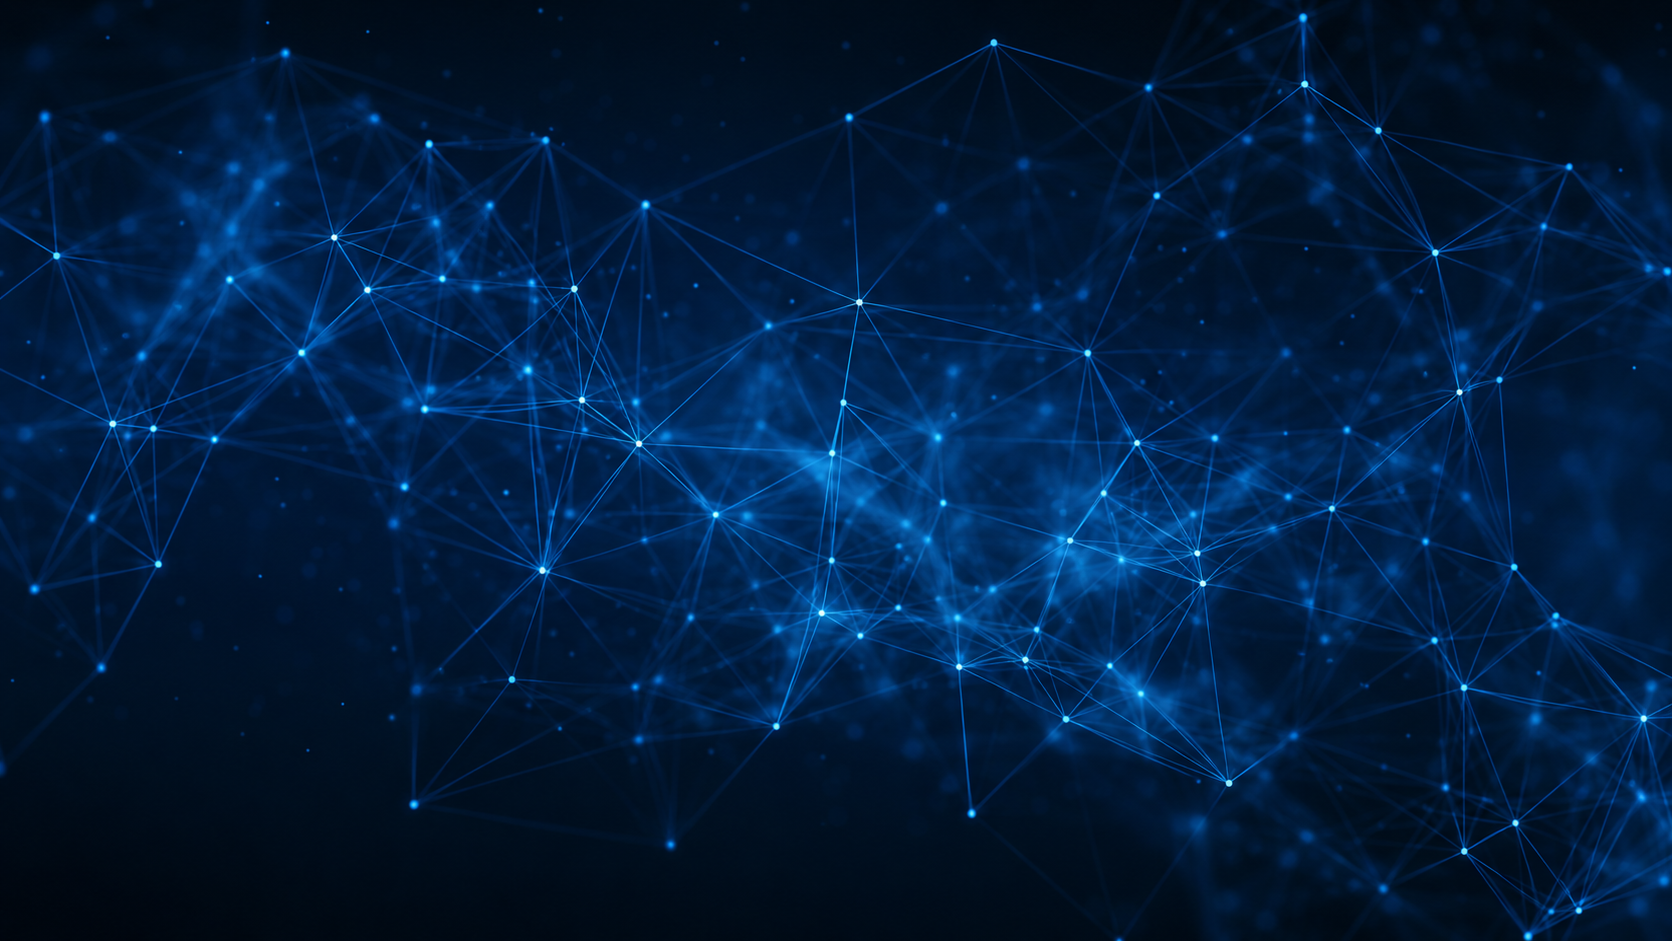
\includegraphics[
        width=\paperwidth,
        height=\paperheight
    ]{121.png}
};

% --------------------------------------------------
% Dark Overlay
% --------------------------------------------------

\fill[
    DarkBlue,
    opacity=0.72
]
(current page.south west)
rectangle
(current page.north east);

% --------------------------------------------------
% Slide Number
% --------------------------------------------------

\node[
    anchor=west,
    text=TechYellow,
    font=\fontsize{14}{16}\selectfont\bfseries
]
at ([xshift=0.8cm,yshift=-0.65cm]
    current page.north west)
{
    08
};

% --------------------------------------------------
% Slide Title
% --------------------------------------------------

\node[
    anchor=west,
    text=White,
    font=\fontsize{18}{22}\selectfont\bfseries
]
at ([xshift=1.8cm,yshift=-0.65cm]
    current page.north west)
{
    Edge Computing Architecture
};

% --------------------------------------------------
% Centered Architecture Diagram Container (Edg_white.png)
% --------------------------------------------------

\node[
    anchor=north,
    draw=TechCyan,
    line width=1.0pt,
    rounded corners=8pt,
    fill=White,
    fill opacity=1,
    text opacity=1,
    inner sep=6pt
]
at ([yshift=-1.20cm]
    current page.north)
{
    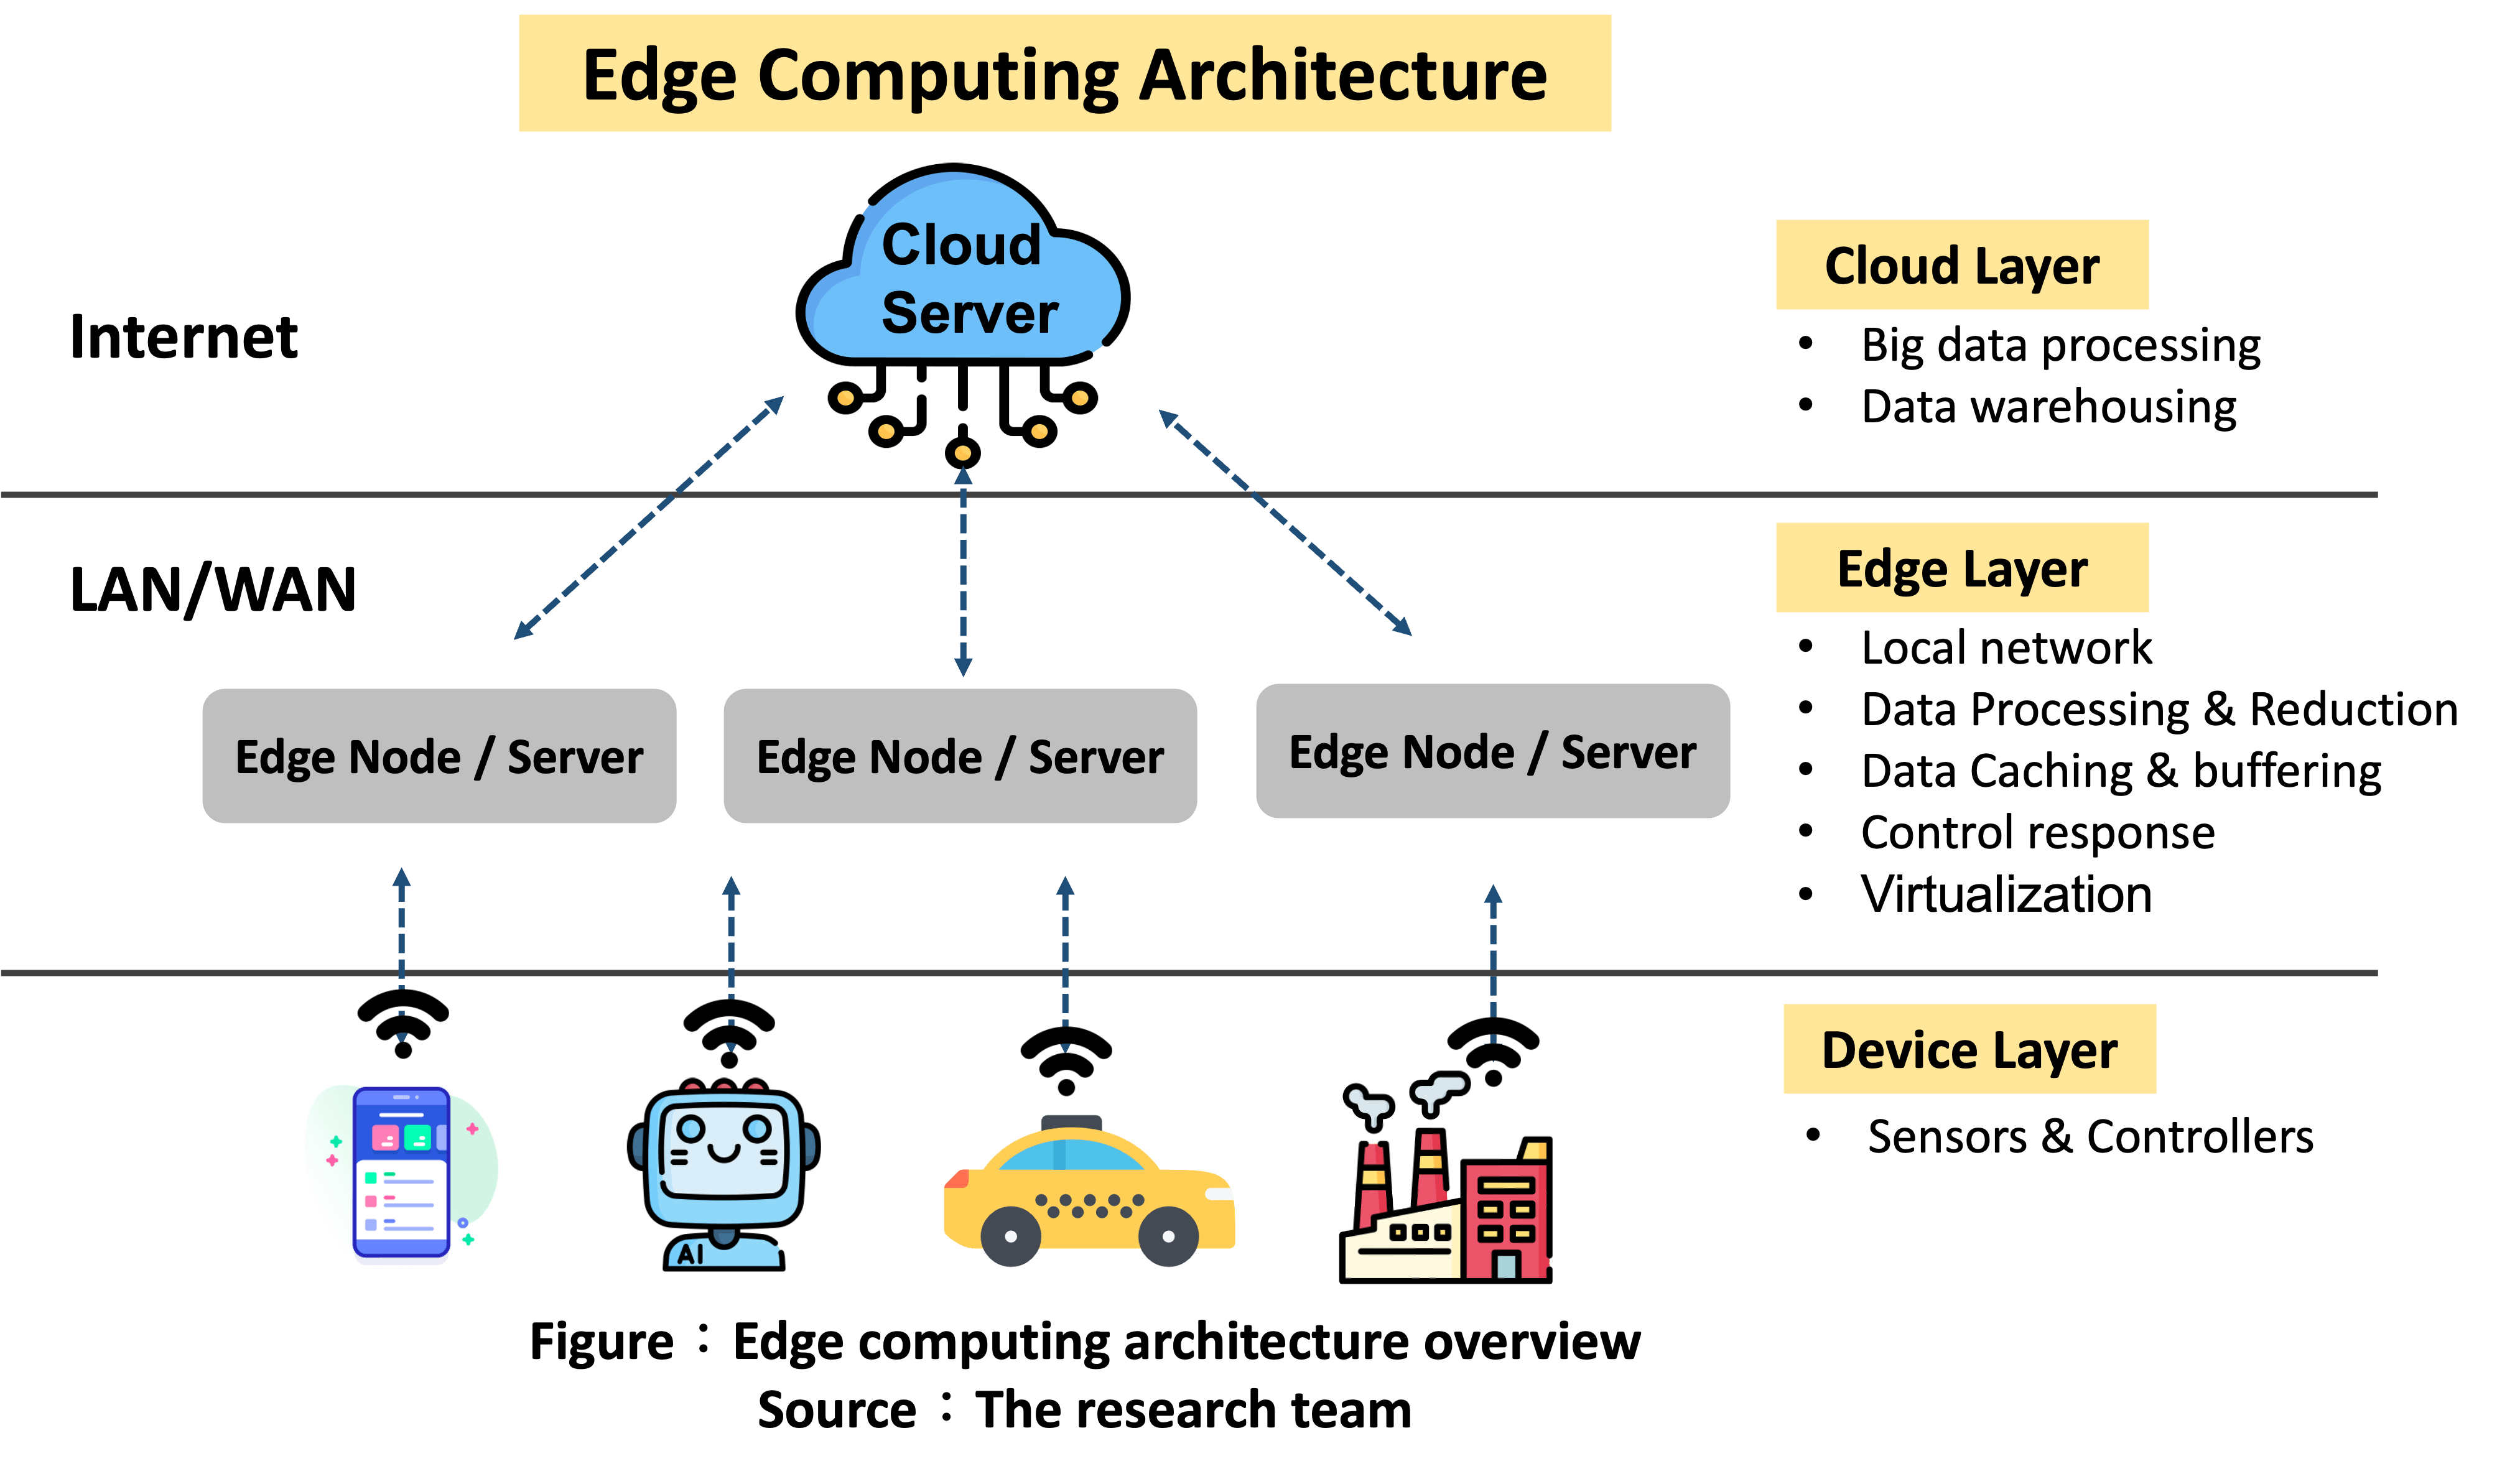
\includegraphics[
        width=13.0cm,
        height=6.2cm,
        keepaspectratio
    ]{Edg_white.png}
};

\end{tikzpicture}

\end{frame}


% ==================================================
% SLIDE 09
% EDGE--CLOUD CONTINUUM
% ==================================================

\begin{frame}[plain]

\begin{tikzpicture}[remember picture,overlay]

% --------------------------------------------------
% Background
% --------------------------------------------------

\node[
    anchor=south west,
    inner sep=0pt
]
at (current page.south west)
{
    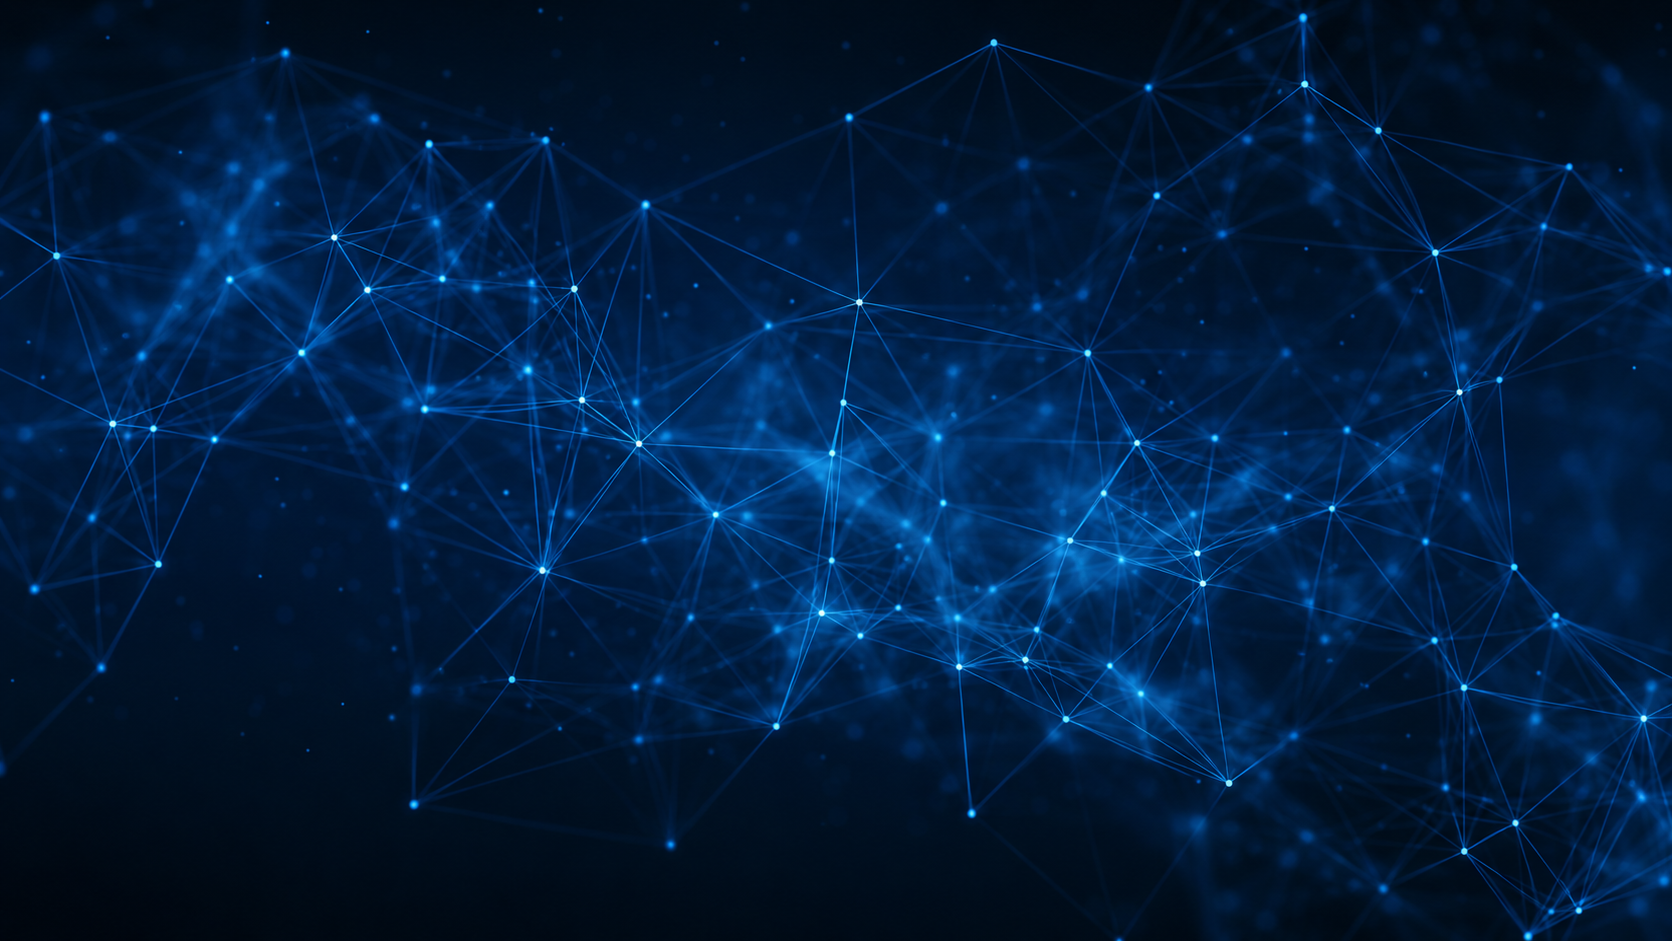
\includegraphics[
        width=\paperwidth,
        height=\paperheight
    ]{121.png}
};

% --------------------------------------------------
% Dark Overlay
% --------------------------------------------------

\fill[
    DarkBlue,
    opacity=0.72
]
(current page.south west)
rectangle
(current page.north east);

% --------------------------------------------------
% Slide Number
% --------------------------------------------------

\node[
    anchor=west,
    text=TechYellow,
    font=\fontsize{14}{16}\selectfont\bfseries
]
at ([xshift=0.8cm,yshift=-0.65cm]
    current page.north west)
{
    09
};

% --------------------------------------------------
% Slide Title
% --------------------------------------------------

\node[
    anchor=west,
    text=White,
    font=\fontsize{18}{22}\selectfont\bfseries
]
at ([xshift=1.8cm,yshift=-0.65cm]
    current page.north west)
{
    Edge--Cloud Continuum
};

% --------------------------------------------------
% Definition Container
% --------------------------------------------------

\node[
    anchor=north west,
    draw=TechCyan,
    line width=0.8pt,
    rounded corners=6pt,
    fill=BoxBlue,
    fill opacity=0.95,
    text opacity=1,
    text width=14.0cm,
    inner xsep=0.35cm,
    inner ysep=0.22cm
]
at ([xshift=0.8cm,yshift=-1.25cm]
    current page.north west)
{
    \textcolor{SoftWhite}{
        \fontsize{10.5}{15}\selectfont
        The \textbf{Edge--Cloud Continuum} is a distributed computing environment in which computing, storage, and services are distributed across IoT devices, edge infrastructure, and centralized cloud resources.
    }
};

% --------------------------------------------------
% Why a Continuum Container
% --------------------------------------------------

\node[
    anchor=north west,
    draw=TechYellow,
    line width=0.8pt,
    rounded corners=6pt,
    fill=BoxBlue,
    fill opacity=0.95,
    text opacity=1,
    text width=14.0cm,
    inner xsep=0.35cm,
    inner ysep=0.25cm
]
at ([xshift=0.8cm,yshift=-3.25cm]
    current page.north west)
{
    \textcolor{TechYellow}{
        \fontsize{12}{15}\selectfont\bfseries
        Why a Continuum?
    }

    \par\vspace{0.15cm}

    \textcolor{SoftWhite}{
        \fontsize{10.5}{15}\selectfont
        Modern IoT applications can involve heterogeneous devices, dynamic workloads, and different performance requirements. This creates the need for efficient task placement, resource allocation, and service orchestration across the IoT--Edge--Cloud environment.
    }
};

% --------------------------------------------------
% Key Principle Banner (At Bottom Space)
% --------------------------------------------------

\node[
    anchor=north west,
    draw=TechCyan,
    line width=0.8pt,
    rounded corners=6pt,
    fill=DarkBlue,
    fill opacity=0.95,
    text opacity=1,
    text width=14.0cm,
    align=center,
    inner xsep=0.25cm,
    inner ysep=0.20cm
]
at ([xshift=0.8cm,yshift=-7.15cm]
    current page.north west)
{
    \textcolor{TechYellow}{\fontsize{10}{13}\selectfont\bfseries Key Principle:}\;\;
    \textcolor{White}{\fontsize{10}{13}\selectfont
    Computation is distributed across the continuum according to application requirements.
    }
};

\end{tikzpicture}

\end{frame}


% ==================================================
% SLIDE 10
% TECHNOLOGIES ENABLING EDGE COMPUTING
% ==================================================

\begin{frame}[plain]

\begin{tikzpicture}[remember picture,overlay]

% --------------------------------------------------
% Background
% --------------------------------------------------

\node[
    anchor=south west,
    inner sep=0pt
]
at (current page.south west)
{
    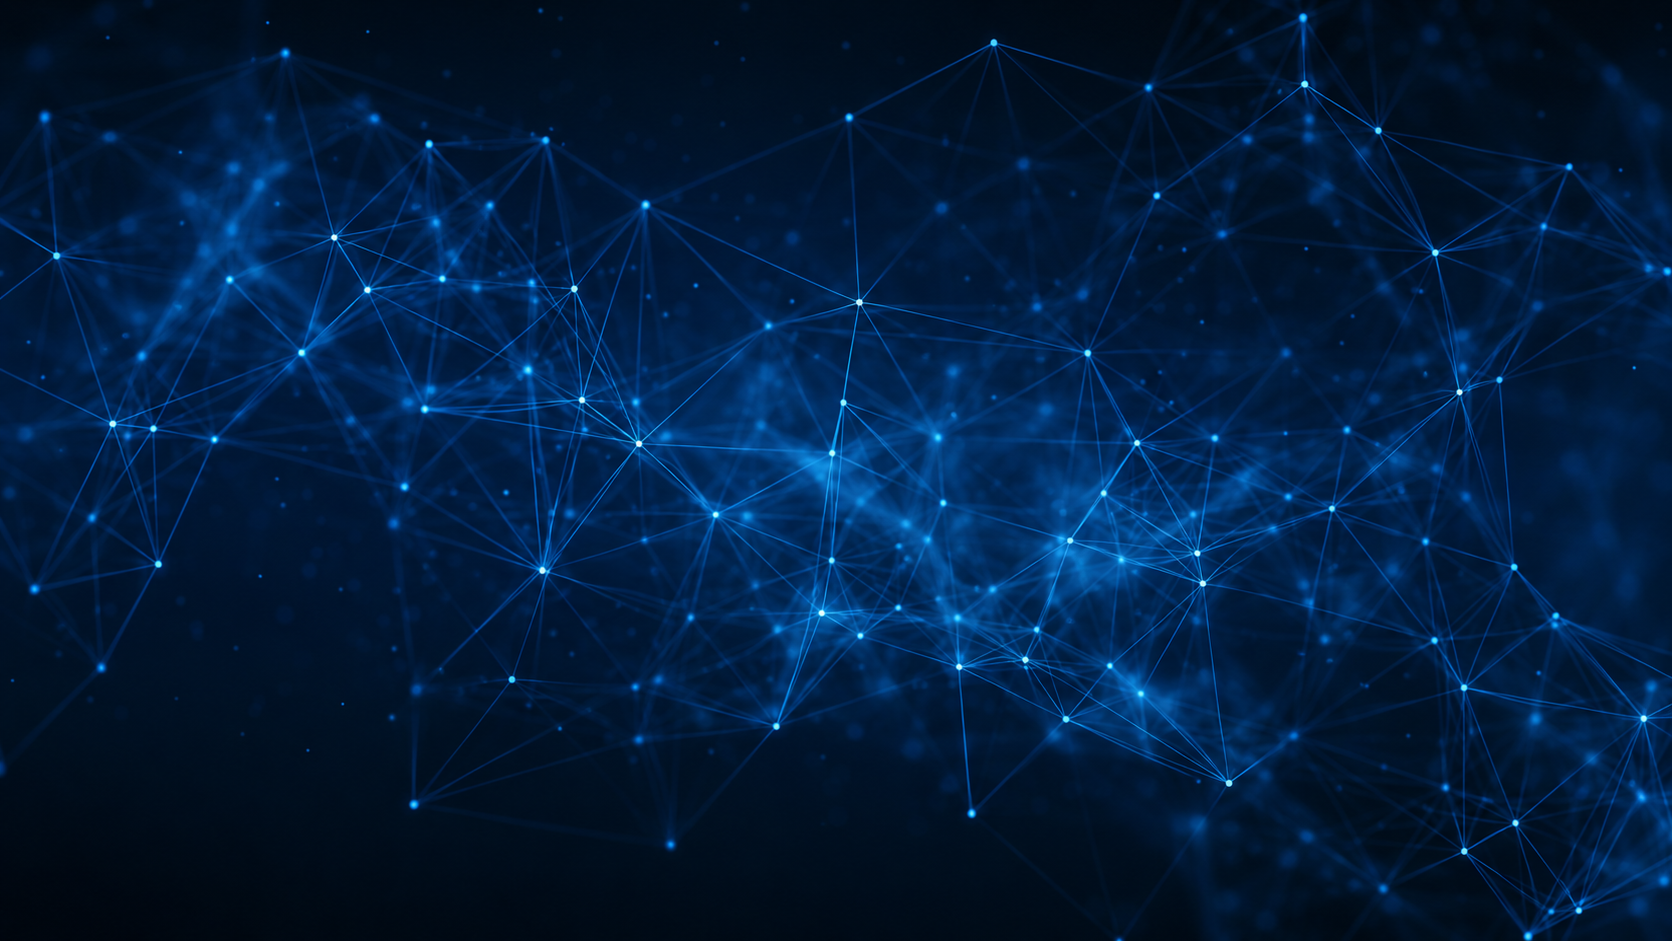
\includegraphics[
        width=\paperwidth,
        height=\paperheight
    ]{121.png}
};

% --------------------------------------------------
% Dark Overlay
% --------------------------------------------------

\fill[
    DarkBlue,
    opacity=0.72
]
(current page.south west)
rectangle
(current page.north east);

% --------------------------------------------------
% Slide Number
% --------------------------------------------------

\node[
    anchor=west,
    text=TechYellow,
    font=\fontsize{14}{16}\selectfont\bfseries
]
at ([xshift=0.8cm,yshift=-0.65cm]
    current page.north west)
{
    10
};

% --------------------------------------------------
% Slide Title
% --------------------------------------------------

\node[
    anchor=west,
    text=White,
    font=\fontsize{18}{22}\selectfont\bfseries
]
at ([xshift=1.8cm,yshift=-0.65cm]
    current page.north west)
{
    Technologies Enabling Edge Computing
};

% --------------------------------------------------
% Item 1: IoT Sensors and Devices
% --------------------------------------------------

\node[
    anchor=north west,
    text width=14.4cm,
    inner sep=0pt
]
at ([xshift=0.8cm,yshift=-1.20cm]
    current page.north west)
{
    \textcolor{TechYellow}{\fontsize{10.5}{13}\selectfont\bfseries 1. IoT Sensors and Devices}\\[2.5pt]
    \textcolor{SoftWhite}{\fontsize{9}{12.5}\selectfont Generate data from the physical environment and provide the input for edge processing.}\\[1.5pt]
    \textcolor{TechCyan}{\fontsize{8.5}{11.5}\selectfont Example: Temperature sensors, cameras, smart meters.}
};

% --------------------------------------------------
% Item 2: High-Speed Networks
% --------------------------------------------------

\node[
    anchor=north west,
    text width=14.4cm,
    inner sep=0pt
]
at ([xshift=0.8cm,yshift=-2.75cm]
    current page.north west)
{
    \textcolor{TechYellow}{\fontsize{10.5}{13}\selectfont\bfseries 2. High-Speed Networks}\\[2.5pt]
    \textcolor{SoftWhite}{\fontsize{9}{12.5}\selectfont Technologies such as 5G, Wi-Fi 6, and Ethernet provide fast and reliable communication between IoT devices and edge nodes.}
};

% --------------------------------------------------
% Item 3: Edge Devices
% --------------------------------------------------

\node[
    anchor=north west,
    text width=14.4cm,
    inner sep=0pt
]
at ([xshift=0.8cm,yshift=-4.15cm]
    current page.north west)
{
    \textcolor{TechYellow}{\fontsize{10.5}{13}\selectfont\bfseries 3. Edge Devices}\\[2.5pt]
    \textcolor{SoftWhite}{\fontsize{9}{12.5}\selectfont Devices such as IoT gateways, routers, Raspberry Pi, and edge servers provide computing capabilities close to the data source.}
};

% --------------------------------------------------
% Item 4: Cloud Computing
% --------------------------------------------------

\node[
    anchor=north west,
    text width=14.4cm,
    inner sep=0pt
]
at ([xshift=0.8cm,yshift=-5.60cm]
    current page.north west)
{
    \textcolor{TechYellow}{\fontsize{10.5}{13}\selectfont\bfseries 4. Cloud Computing}\\[2.5pt]
    \textcolor{SoftWhite}{\fontsize{9}{12.5}\selectfont The cloud works together with edge infrastructure for large-scale storage, complex processing, and long-term analytics.}
};

% --------------------------------------------------
% Item 5: Artificial Intelligence and Machine Learning (Bottom Space)
% --------------------------------------------------

\node[
    anchor=north west,
    text width=14.4cm,
    inner sep=0pt
]
at ([xshift=0.8cm,yshift=-7.05cm]
    current page.north west)
{
    \textcolor{TechYellow}{\fontsize{10.5}{13}\selectfont\bfseries 5. Artificial Intelligence and Machine Learning}\\[2.5pt]
    \textcolor{SoftWhite}{\fontsize{9}{12.5}\selectfont AI/ML allows edge systems to analyze data and make decisions locally, without sending every piece of data to the cloud.}
};

\end{tikzpicture}

\end{frame}


% ==================================================
% SLIDE 11
% EDGE AI
% ==================================================

\begin{frame}[plain]

\begin{tikzpicture}[remember picture,overlay]

% --------------------------------------------------
% Background
% --------------------------------------------------

\node[
    anchor=south west,
    inner sep=0pt
]
at (current page.south west)
{
    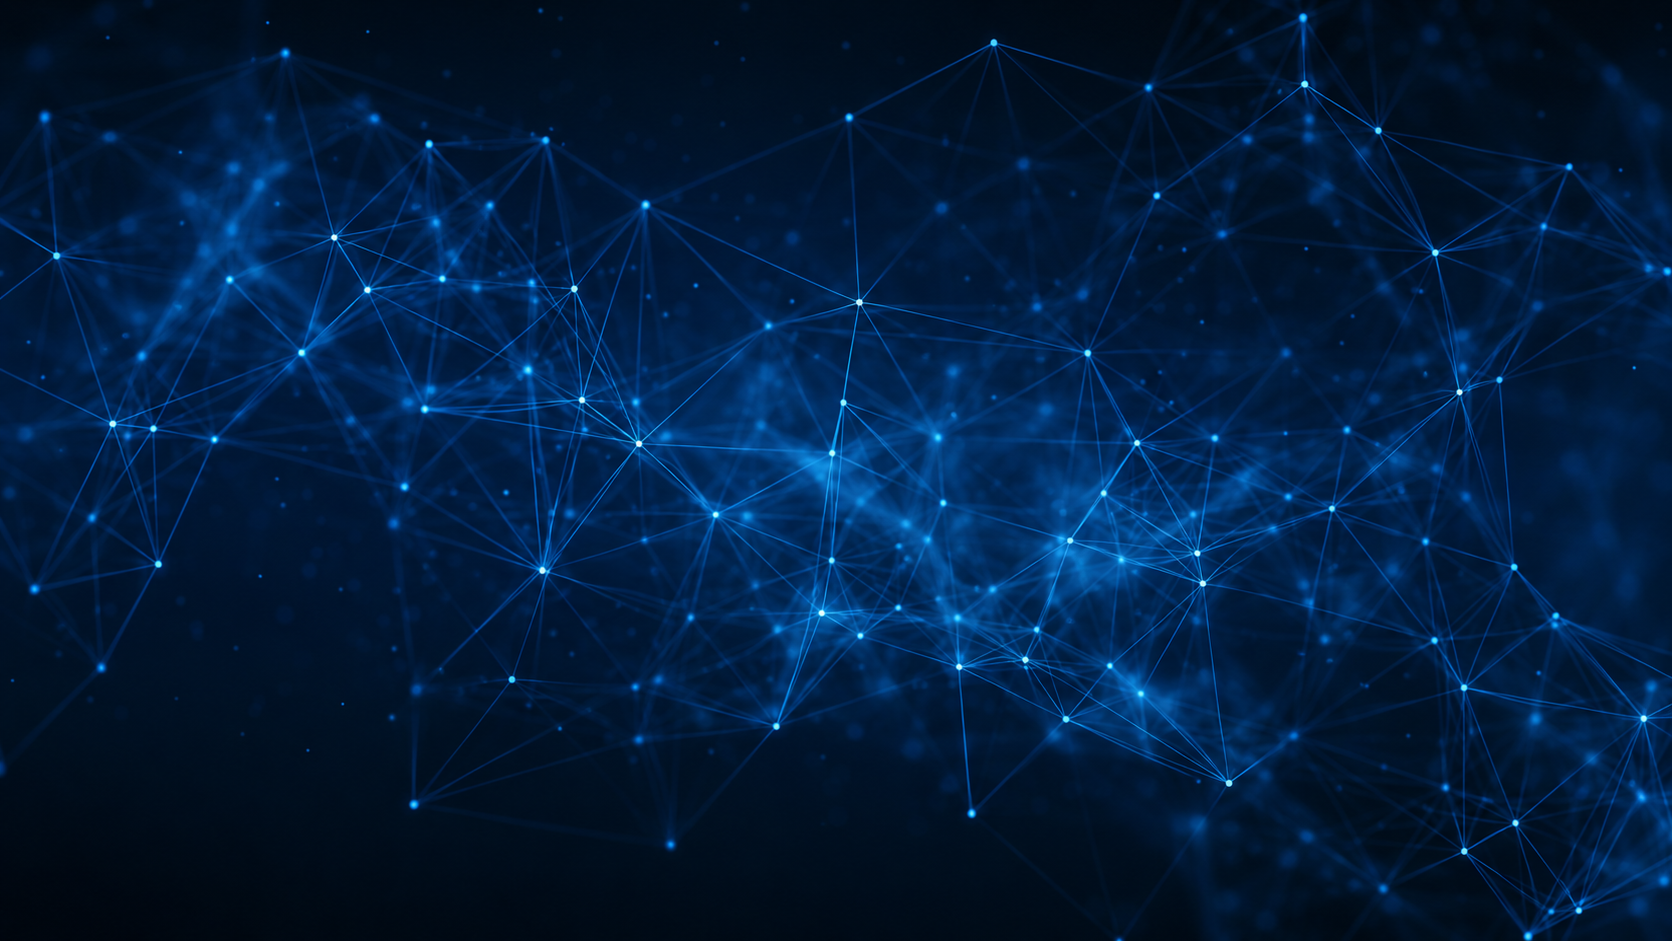
\includegraphics[
        width=\paperwidth,
        height=\paperheight
    ]{121.png}
};

% --------------------------------------------------
% Dark Overlay
% --------------------------------------------------

\fill[
    DarkBlue,
    opacity=0.72
]
(current page.south west)
rectangle
(current page.north east);

% --------------------------------------------------
% Slide Number
% --------------------------------------------------

\node[
    anchor=west,
    text=TechYellow,
    font=\fontsize{14}{16}\selectfont\bfseries
]
at ([xshift=0.8cm,yshift=-0.65cm]
    current page.north west)
{
    11
};

% --------------------------------------------------
% Slide Title
% --------------------------------------------------

\node[
    anchor=west,
    text=White,
    font=\fontsize{18}{22}\selectfont\bfseries
]
at ([xshift=1.8cm,yshift=-0.65cm]
    current page.north west)
{
    Edge AI
};

% --------------------------------------------------
% Top Definition Card: What is Edge AI?
% --------------------------------------------------

\node[
    anchor=north west,
    draw=TechCyan,
    line width=0.8pt,
    rounded corners=6pt,
    fill=BoxBlue,
    fill opacity=0.95,
    text opacity=1,
    text width=14.4cm,
    inner xsep=0.30cm,
    inner ysep=0.12cm
]
at ([xshift=0.8cm,yshift=-1.15cm]
    current page.north west)
{
    \textcolor{TechYellow}{\fontsize{10.5}{13}\selectfont\bfseries What is Edge AI?}\\[3pt]
    \textcolor{SoftWhite}{\fontsize{9}{12.5}\selectfont
    Edge AI refers to the deployment of Artificial Intelligence and Machine Learning capabilities at or near the network edge, allowing data to be processed and AI inference to be performed close to where the data is generated.\\[3pt]
    For IoT applications that require rapid responses, this can introduce latency, network dependency, and unnecessary data transmission.
    }
};

% --------------------------------------------------
% Side-by-Side Advantage Cards (Stretched to Bottom)
% --------------------------------------------------

% Left Card: Performance & Efficiency
\node[
    anchor=north west,
    draw=TechYellow,
    line width=0.8pt,
    rounded corners=6pt,
    fill=BoxBlue,
    fill opacity=0.95,
    text opacity=1,
    text width=6.6cm,
    minimum height=3.90cm,
    inner xsep=0.30cm,
    inner ysep=0.18cm
]
at ([xshift=0.8cm,yshift=-4.20cm]
    current page.north west)
{
    \textcolor{TechYellow}{\fontsize{10.5}{13}\selectfont\bfseries Performance \& Efficiency}\\[5pt]
    \textcolor{TechCyan}{$\bullet$}\;\;\textcolor{White}{\fontsize{9}{12}\selectfont\bfseries Real-Time Inference:}\\[1.5pt]
    \hspace*{0.30cm}\textcolor{SoftWhite}{\fontsize{8.5}{11}\selectfont Performed directly closer to the data source.}\\[5pt]
    \textcolor{TechCyan}{$\bullet$}\;\;\textcolor{White}{\fontsize{9}{12}\selectfont\bfseries Reduced Latency:}\\[1.5pt]
    \hspace*{0.30cm}\textcolor{SoftWhite}{\fontsize{8.5}{11}\selectfont Essential for time-sensitive applications.}\\[5pt]
    \textcolor{TechCyan}{$\bullet$}\;\;\textcolor{White}{\fontsize{9}{12}\selectfont\bfseries Data Transmission:}\\[1.5pt]
    \hspace*{0.30cm}\textcolor{SoftWhite}{\fontsize{8.5}{11}\selectfont Minimizes data sent to centralized cloud systems.}
};

% Right Card: Privacy & Reliability
\node[
    anchor=north west,
    draw=TechCyan,
    line width=0.8pt,
    rounded corners=6pt,
    fill=BoxBlue,
    fill opacity=0.95,
    text opacity=1,
    text width=6.6cm,
    minimum height=3.90cm,
    inner xsep=0.30cm,
    inner ysep=0.18cm
]
at ([xshift=8.2cm,yshift=-4.20cm]
    current page.north west)
{
    \textcolor{TechCyan}{\fontsize{10.5}{13}\selectfont\bfseries Privacy \& Reliability}\\[6pt]
    \textcolor{TechCyan}{$\bullet$}\;\;\textcolor{White}{\fontsize{9}{12}\selectfont\bfseries Improved Privacy:}\\[1.5pt]
    \hspace*{0.30cm}\textcolor{SoftWhite}{\fontsize{8.5}{11}\selectfont Keeps sensitive data stored and processed locally.}\\[6pt]
    \textcolor{TechCyan}{$\bullet$}\;\;\textcolor{White}{\fontsize{8.5}{11}\selectfont\bfseries Continuous Operation:}\\[1.5pt]
    \hspace*{0.30cm}\textcolor{SoftWhite}{\fontsize{8.5}{11}\selectfont Operates seamlessly even when cloud connectivity is limited.}
};

\end{tikzpicture}

\end{frame}


% ==================================================
% SLIDE 12
% EXAMPLE: AUTONOMOUS VEHICLES (2-COLUMN SPLIT SHOWCASE)
% ==================================================

\begin{frame}[plain]

\begin{tikzpicture}[remember picture,overlay]

% --------------------------------------------------
% Background
% --------------------------------------------------

\node[
    anchor=south west,
    inner sep=0pt
]
at (current page.south west)
{
    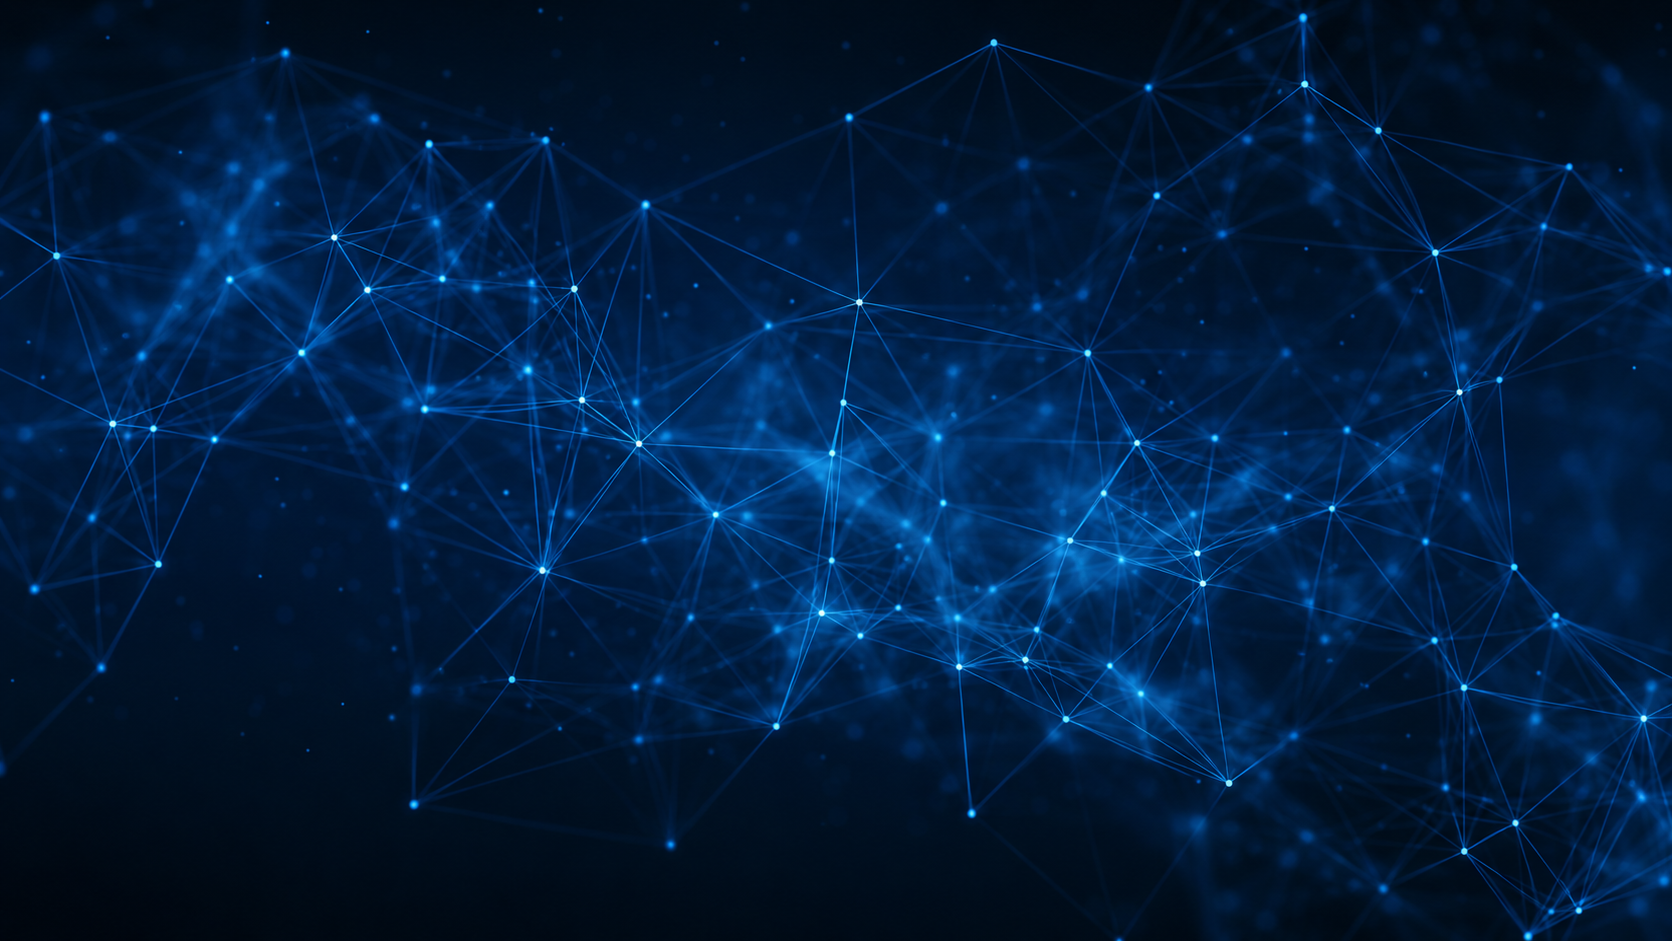
\includegraphics[
        width=\paperwidth,
        height=\paperheight
    ]{121.png}
};

% --------------------------------------------------
% Dark Overlay
% --------------------------------------------------

\fill[
    DarkBlue,
    opacity=0.72
]
(current page.south west)
rectangle
(current page.north east);

% --------------------------------------------------
% Slide Number
% --------------------------------------------------

\node[
    anchor=west,
    text=TechYellow,
    font=\fontsize{14}{16}\selectfont\bfseries
]
at ([xshift=0.8cm,yshift=-0.65cm]
    current page.north west)
{
    12
};

% --------------------------------------------------
% Slide Title
% --------------------------------------------------

\node[
    anchor=west,
    text=White,
    font=\fontsize{18}{22}\selectfont\bfseries
]
at ([xshift=1.8cm,yshift=-0.65cm]
    current page.north west)
{
    Example
};

% --------------------------------------------------
% Left Column: Context & Key Requirements Card
% --------------------------------------------------

\node[
    anchor=north west,
    draw=TechYellow,
    line width=0.8pt,
    rounded corners=6pt,
    fill=BoxBlue,
    fill opacity=0.95,
    text opacity=1,
    text width=5.2cm,
    minimum height=6.45cm,
    inner xsep=0.28cm,
    inner ysep=0.25cm
]
at ([xshift=0.8cm,yshift=-1.15cm]
    current page.north west)
{
    \textcolor{TechYellow}{\fontsize{10.5}{13}\selectfont\bfseries Autonomous Vehicles}\\[8pt]
    \textcolor{SoftWhite}{\fontsize{8.5}{12}\selectfont
    Autonomous Vehicles are a key application of Edge AI, where AI models process sensor data locally to enable real-time perception and decision-making.\\[12pt]
    \textcolor{TechCyan}{$\bullet$}\;\;\textcolor{White}{\bfseries Sub-ms Response:}\\[2pt]
    \hspace*{0.25cm}Zero cloud round-trip delay.\\[8pt]
    \textcolor{TechCyan}{$\bullet$}\;\;\textcolor{White}{\bfseries Safety Critical:}\\[2pt]
    \hspace*{0.25cm}Guaranteed offline execution.
    }
};

% --------------------------------------------------
% Right Column: Embedded AV Pipeline Diagram Figure
% --------------------------------------------------

\node[
    anchor=north west,
    draw=TechCyan,
    line width=0.8pt,
    rounded corners=6pt,
    fill=White,
    text width=8.1cm,
    minimum height=6.45cm,
    align=center,
    inner xsep=0.15cm,
    inner ysep=0.15cm
]
at ([xshift=6.6cm,yshift=-1.15cm]
    current page.north west)
{
    \vfill
    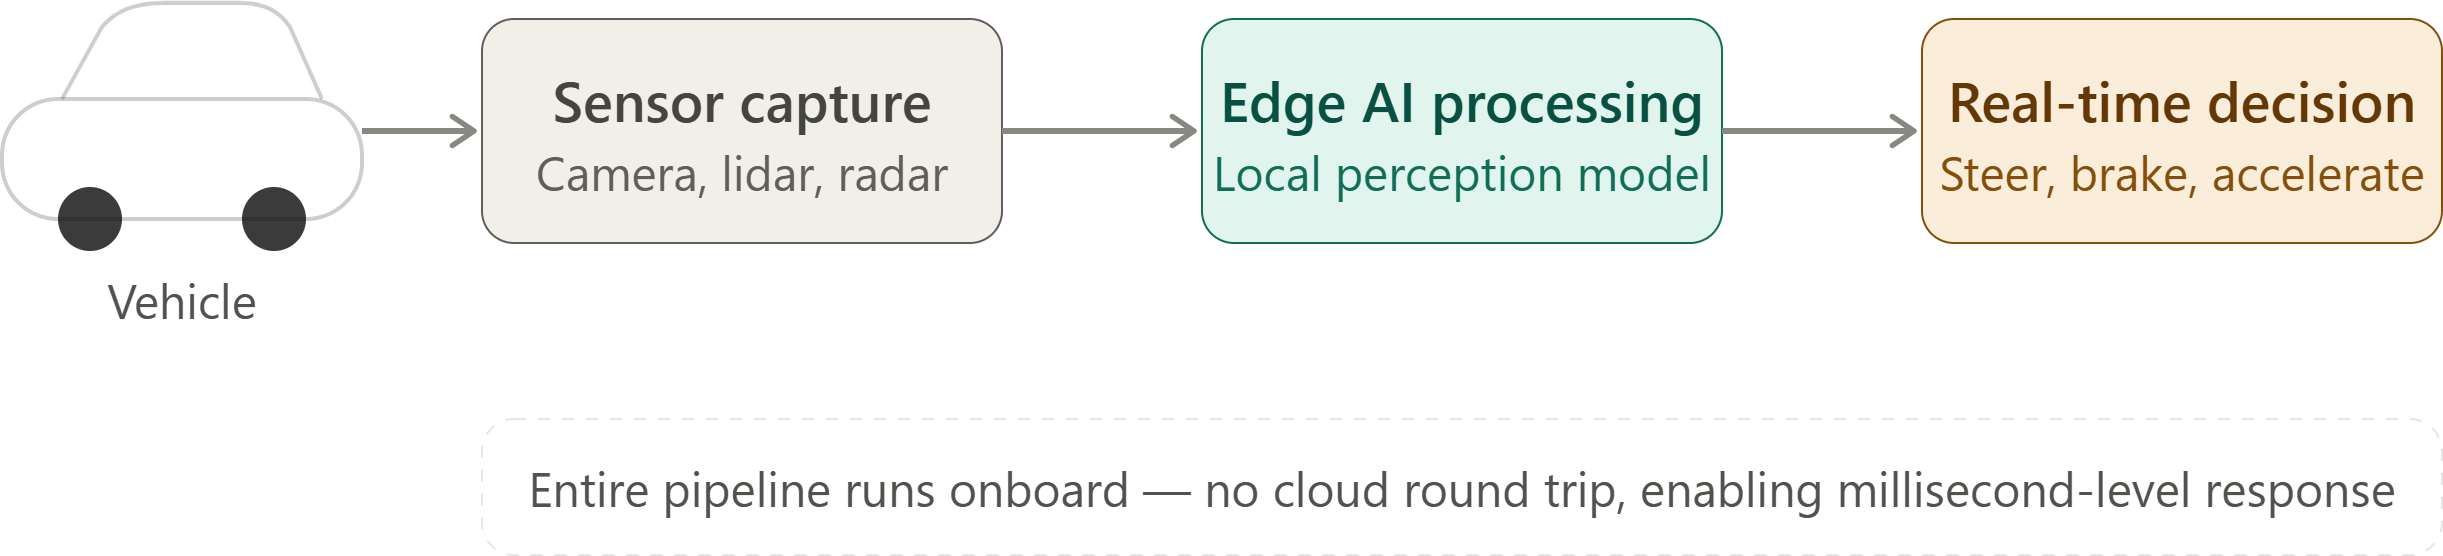
\includegraphics[
        width=8.0cm,
        height=5.8cm,
        keepaspectratio
    ]{edge_ai_av_pipeline_cropped.png}
    \vfill
};

% --------------------------------------------------
% Bottom Banner: Sensor-to-Decision Decision Pipeline
% --------------------------------------------------

\node[
    anchor=north west,
    draw=TechCyan,
    line width=0.8pt,
    rounded corners=6pt,
    fill=DarkBlue,
    fill opacity=0.95,
    text opacity=1,
    text width=14.4cm,
    align=center,
    inner xsep=0.20cm,
    inner ysep=0.16cm
]
at ([xshift=0.8cm,yshift=-7.80cm]
    current page.north west)
{
    \textcolor{TechYellow}{\fontsize{9}{11}\selectfont\bfseries Pipeline Sequence:}\;\;
    \textcolor{White}{\fontsize{8}{10}\selectfont
    \textbf{Camera / Sensors} $\;\longrightarrow\;$ \textbf{\textcolor{TechCyan}{Edge AI}} $\;\longrightarrow\;$ \textbf{Object Detection} $\;\longrightarrow\;$ \textbf{\textcolor{TechYellow}{Steering / Braking Decision}}
    }
};

\end{tikzpicture}

\end{frame}


% ==================================================
% SLIDE 13
% APPLICATIONS OF EDGE COMPUTING (6-CARD GRID SHOWCASE)
% ==================================================

\begin{frame}[plain]

\begin{tikzpicture}[remember picture,overlay]

% --------------------------------------------------
% Background
% --------------------------------------------------

\node[
    anchor=south west,
    inner sep=0pt
]
at (current page.south west)
{
    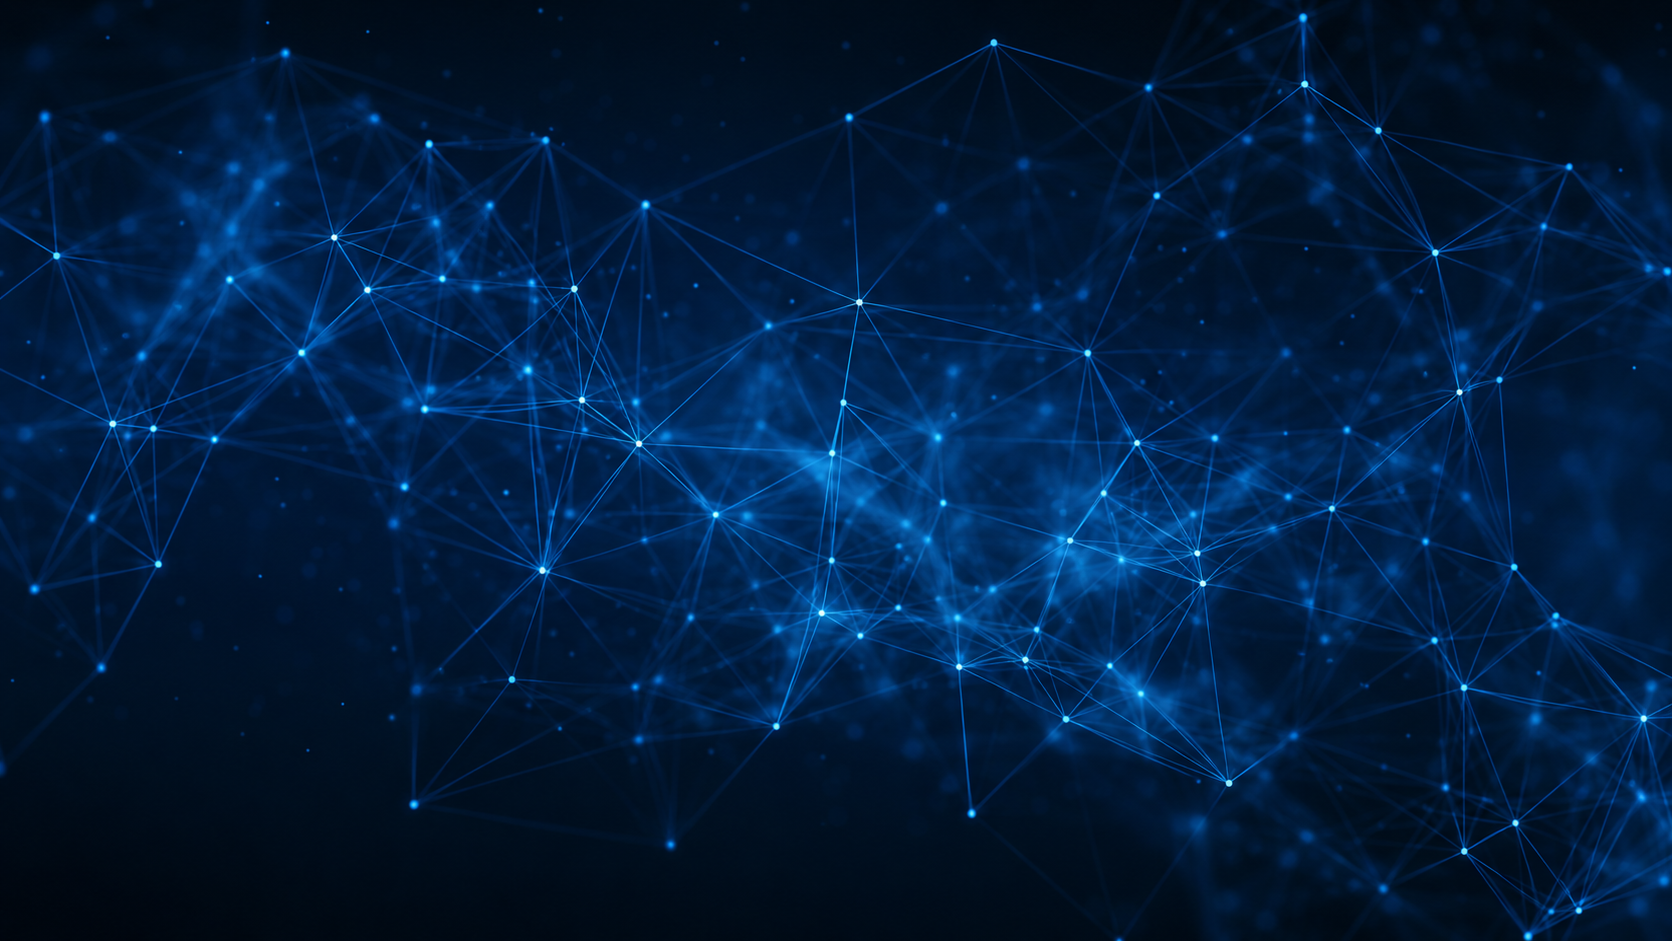
\includegraphics[
        width=\paperwidth,
        height=\paperheight
    ]{121.png}
};

% --------------------------------------------------
% Dark Overlay
% --------------------------------------------------

\fill[
    DarkBlue,
    opacity=0.72
]
(current page.south west)
rectangle
(current page.north east);

% --------------------------------------------------
% Slide Number
% --------------------------------------------------

\node[
    anchor=west,
    text=TechYellow,
    font=\fontsize{14}{16}\selectfont\bfseries
]
at ([xshift=0.8cm,yshift=-0.65cm]
    current page.north west)
{
    13
};

% --------------------------------------------------
% Slide Title
% --------------------------------------------------

\node[
    anchor=west,
    text=White,
    font=\fontsize{18}{22}\selectfont\bfseries
]
at ([xshift=1.8cm,yshift=-0.65cm]
    current page.north west)
{
    Applications of Edge Computing
};

% --------------------------------------------------
% Subtitle Summary Line (Unboxed for zero clutter)
% --------------------------------------------------

\node[
    anchor=north west,
    text width=14.8cm,
    inner sep=0pt
]
at ([xshift=0.8cm,yshift=-1.10cm] current page.north west)
{
    \textcolor{SoftWhite}{\fontsize{8.2}{11}\selectfont
    Edge Computing is particularly useful for applications requiring low latency, local processing, and efficient data delivery.
    }
};

% Top Accent Divider Line
\draw[TechCyan, line width=0.8pt, opacity=0.6]
    ([xshift=0.8cm,yshift=-1.50cm] current page.north west) --
    ([xshift=15.2cm,yshift=-1.50cm] current page.north west);

% ==================================================
% ROW 1: CARDS 1-3
% ==================================================

% Card 1: Video Caching
\node[
    anchor=north west,
    draw=TechCyan,
    line width=0.8pt,
    rounded corners=6pt,
    fill=BoxTeal,
    fill opacity=0.95,
    text opacity=1,
    text width=4.20cm,
    minimum height=2.45cm,
    inner xsep=0.18cm,
    inner ysep=0.10cm
]
at ([xshift=0.80cm,yshift=-1.65cm] current page.north west)
{
    \textcolor{TechCyan}{\fontsize{9.5}{12}\selectfont\bfseries Video Caching}\\[3pt]
    \textcolor{SoftWhite}{\fontsize{7.8}{10.2}\selectfont
    Stores popular streaming media closer to end-users to reduce backhaul traffic and playback buffering.
    }
};

% Card 2: 5G & Edge Computing
\node[
    anchor=north west,
    draw=TechYellow,
    line width=0.8pt,
    rounded corners=6pt,
    fill=BoxPurple,
    fill opacity=0.95,
    text opacity=1,
    text width=4.20cm,
    minimum height=2.45cm,
    inner xsep=0.18cm,
    inner ysep=0.10cm
]
at ([xshift=5.70cm,yshift=-1.65cm] current page.north west)
{
    \textcolor{TechYellow}{\fontsize{9.5}{12}\selectfont\bfseries 5G \& Edge Computing}\\[3pt]
    \textcolor{SoftWhite}{\fontsize{7.8}{10.2}\selectfont
    Integrates Multi-access Edge Computing into 5G radio networks for ultra-low latency ($<1$\,ms) services.
    }
};

% Card 3: Live Video Broadcasting
\node[
    anchor=north west,
    draw=TechCyan,
    line width=0.8pt,
    rounded corners=6pt,
    fill=BoxIndigo,
    fill opacity=0.95,
    text opacity=1,
    text width=4.20cm,
    minimum height=2.45cm,
    inner xsep=0.18cm,
    inner ysep=0.10cm
]
at ([xshift=10.60cm,yshift=-1.65cm] current page.north west)
{
    \textcolor{TechCyan}{\fontsize{9.5}{12}\selectfont\bfseries Live Video Broadcasting}\\[3pt]
    \textcolor{SoftWhite}{\fontsize{7.8}{10.2}\selectfont
    Transcodes and processes high-bitrate live video streams locally for real-time low-delay distribution.
    }
};

% ==================================================
% ROW 2: CARDS 4-6
% ==================================================

% Card 4: Predictive Maintenance
\node[
    anchor=north west,
    draw=TechYellow,
    line width=0.8pt,
    rounded corners=6pt,
    fill=BoxEmerald,
    fill opacity=0.95,
    text opacity=1,
    text width=4.20cm,
    minimum height=2.45cm,
    inner xsep=0.18cm,
    inner ysep=0.10cm
]
at ([xshift=0.80cm,yshift=-4.30cm] current page.north west)
{
    \textcolor{TechYellow}{\fontsize{9.5}{12}\selectfont\bfseries Predictive Maintenance}\\[3pt]
    \textcolor{SoftWhite}{\fontsize{7.8}{10.2}\selectfont
    Analyzes industrial IoT sensor metrics on-site to detect equipment anomalies before failures happen.
    }
};

% Card 5: Security Monitoring
\node[
    anchor=north west,
    draw=TechCyan,
    line width=0.8pt,
    rounded corners=6pt,
    fill=BoxWine,
    fill opacity=0.95,
    text opacity=1,
    text width=4.20cm,
    minimum height=2.45cm,
    inner xsep=0.18cm,
    inner ysep=0.10cm
]
at ([xshift=5.70cm,yshift=-4.30cm] current page.north west)
{
    \textcolor{TechCyan}{\fontsize{9.5}{12}\selectfont\bfseries Security Monitoring}\\[3pt]
    \textcolor{SoftWhite}{\fontsize{7.8}{10.2}\selectfont
    Runs local AI video analytics on smart camera feeds for instant threat and intrusion detection.
    }
};

% Card 6: Autonomous Vehicles
\node[
    anchor=north west,
    draw=TechYellow,
    line width=0.8pt,
    rounded corners=6pt,
    fill=BoxSlate,
    fill opacity=0.95,
    text opacity=1,
    text width=4.20cm,
    minimum height=2.45cm,
    inner xsep=0.18cm,
    inner ysep=0.10cm
]
at ([xshift=10.60cm,yshift=-4.30cm] current page.north west)
{
    \textcolor{TechYellow}{\fontsize{9.5}{12}\selectfont\bfseries Autonomous Vehicles}\\[3pt]
    \textcolor{SoftWhite}{\fontsize{7.8}{10.2}\selectfont
    Processes onboard sensor data locally for sub-millisecond perception, steering, and braking controls.
    }
};

\end{tikzpicture}

\end{frame}


% ==================================================
% SLIDE 14
% VIDEO CACHING AT THE EDGE
% ==================================================

\begin{frame}[plain]

\begin{tikzpicture}[remember picture,overlay]

% Background
\node[anchor=south west, inner sep=0pt] at (current page.south west) {
    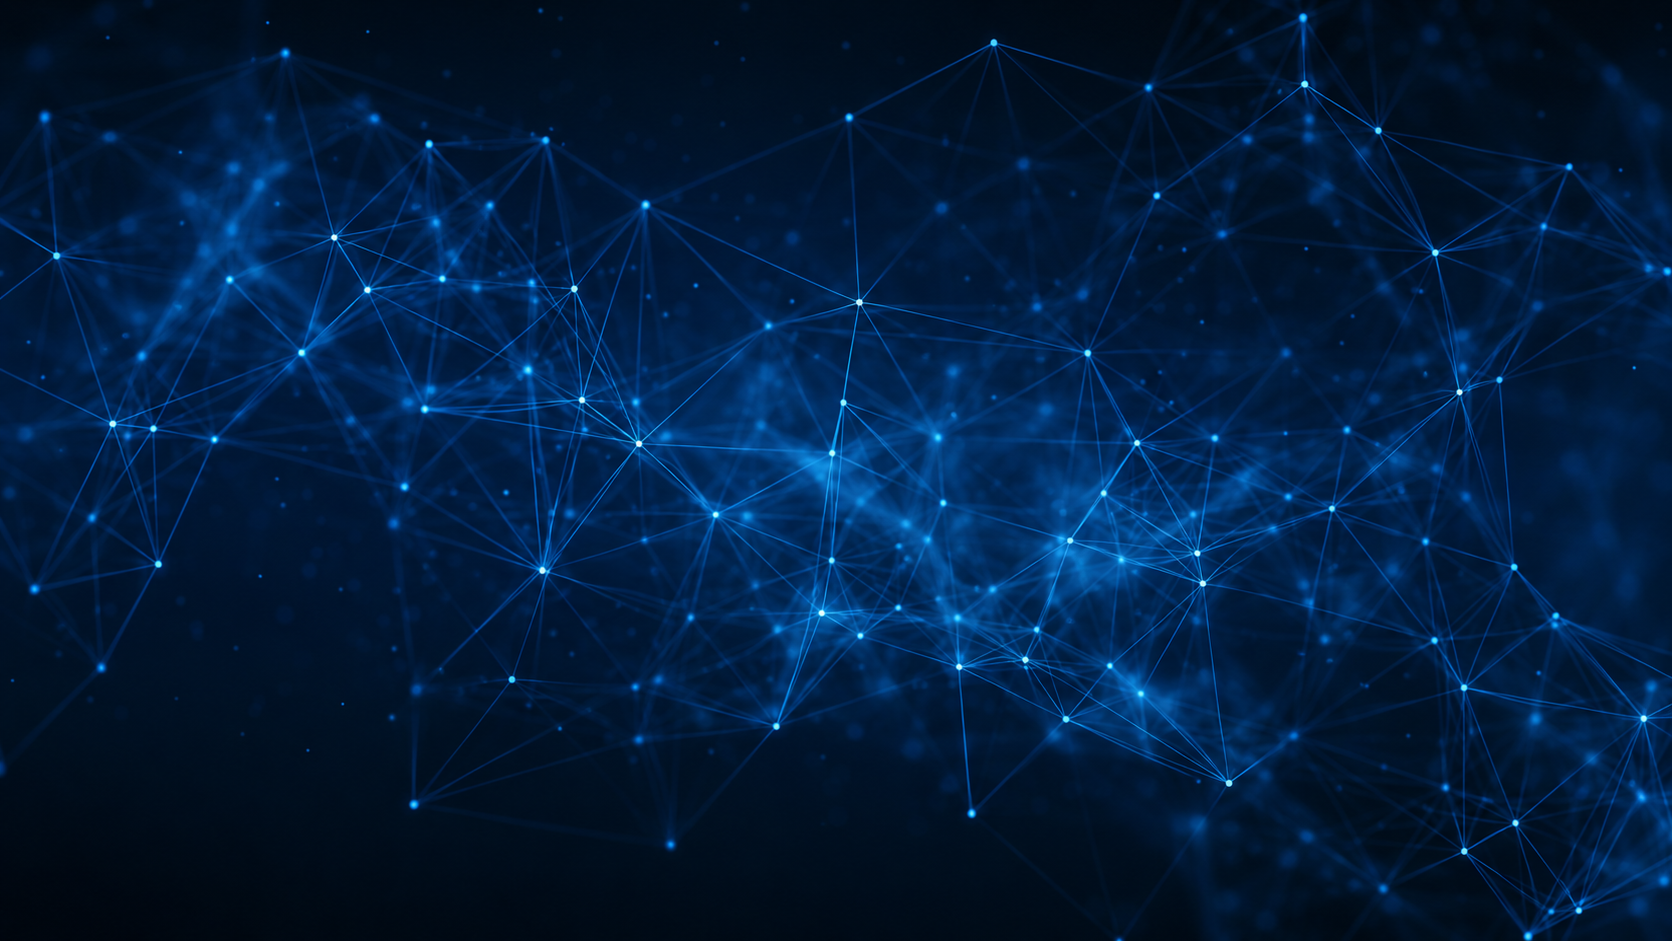
\includegraphics[width=\paperwidth, height=\paperheight]{121.png}
};
\fill[DarkBlue, opacity=0.72] (current page.south west) rectangle (current page.north east);

% Slide Number & Title
\node[anchor=west, text=TechYellow, font=\fontsize{14}{16}\selectfont\bfseries] at ([xshift=0.8cm,yshift=-0.65cm] current page.north west) {14};
\node[anchor=west, text=White, font=\fontsize{18}{22}\selectfont\bfseries] at ([xshift=1.8cm,yshift=-0.65cm] current page.north west) {Video Caching at the Edge};

% Flow Banner
\node[
    anchor=north west,
    draw=TechCyan,
    line width=0.8pt,
    rounded corners=6pt,
    fill=DarkBlue,
    fill opacity=0.95,
    text opacity=1,
    text width=14.4cm,
    align=center,
    inner xsep=0.20cm,
    inner ysep=0.14cm
]
at ([xshift=0.8cm,yshift=-1.15cm] current page.north west)
{
    \textcolor{TechYellow}{\fontsize{9.5}{12}\selectfont\bfseries Data Flow:}\;\;
    \textcolor{White}{\fontsize{9}{12}\selectfont
    \textbf{Popular Content} $\;\longrightarrow\;$ \textbf{\textcolor{TechCyan}{Nearby Edge Server}} $\;\longrightarrow\;$ \textbf{\textcolor{TechYellow}{User}}
    }
};

% Main Feature Box
\node[
    anchor=north west,
    draw=TechYellow,
    line width=0.8pt,
    rounded corners=6pt,
    fill=BoxIndigo,
    fill opacity=0.95,
    text opacity=1,
    text width=14.4cm,
    minimum height=4.20cm,
    inner xsep=0.30cm,
    inner ysep=0.20cm
]
at ([xshift=0.8cm,yshift=-2.15cm] current page.north west)
{
    \textcolor{TechYellow}{\fontsize{11}{14}\selectfont\bfseries Core Video Caching Mechanics}\\[8pt]
    \textcolor{SoftWhite}{\fontsize{9}{13}\selectfont
    \textcolor{TechCyan}{$\bullet$}\;\;\textcolor{White}{\bfseries Proximity Storage:}\;\;
    Frequently requested streaming content is cached directly at localized edge servers near end-users.\\[6pt]
    \textcolor{TechCyan}{$\bullet$}\;\;\textcolor{White}{\bfseries Backhaul Traffic Reduction:}\;\;
    Prevents repeated data transmission across backhaul and core cloud networks.\\[6pt]
    \textcolor{TechCyan}{$\bullet$}\;\;\textcolor{White}{\bfseries Network De-congestion:}\;\;
    Significantly reduces peak network congestion and eliminates video access delays.
    }
};

% Key Benefit Banner
\node[
    anchor=north west,
    draw=TechCyan,
    line width=0.8pt,
    rounded corners=6pt,
    fill=DarkBlue,
    fill opacity=0.95,
    text opacity=1,
    text width=14.4cm,
    align=center,
    inner xsep=0.20cm,
    inner ysep=0.16cm
]
at ([xshift=0.8cm,yshift=-6.75cm] current page.north west)
{
    \textcolor{TechYellow}{\fontsize{9.5}{12}\selectfont\bfseries Key Benefit:}\;\;
    \textcolor{White}{\fontsize{9}{12}\selectfont
    Delivers \textbf{faster video playback} with drastically reduced core network load.
    }
};

\end{tikzpicture}

\end{frame}


% ==================================================
% SLIDE 15
% EDGE COMPUTING AND 5G
% ==================================================

\begin{frame}[plain]

\begin{tikzpicture}[remember picture,overlay]

% Background
\node[anchor=south west, inner sep=0pt] at (current page.south west) {
    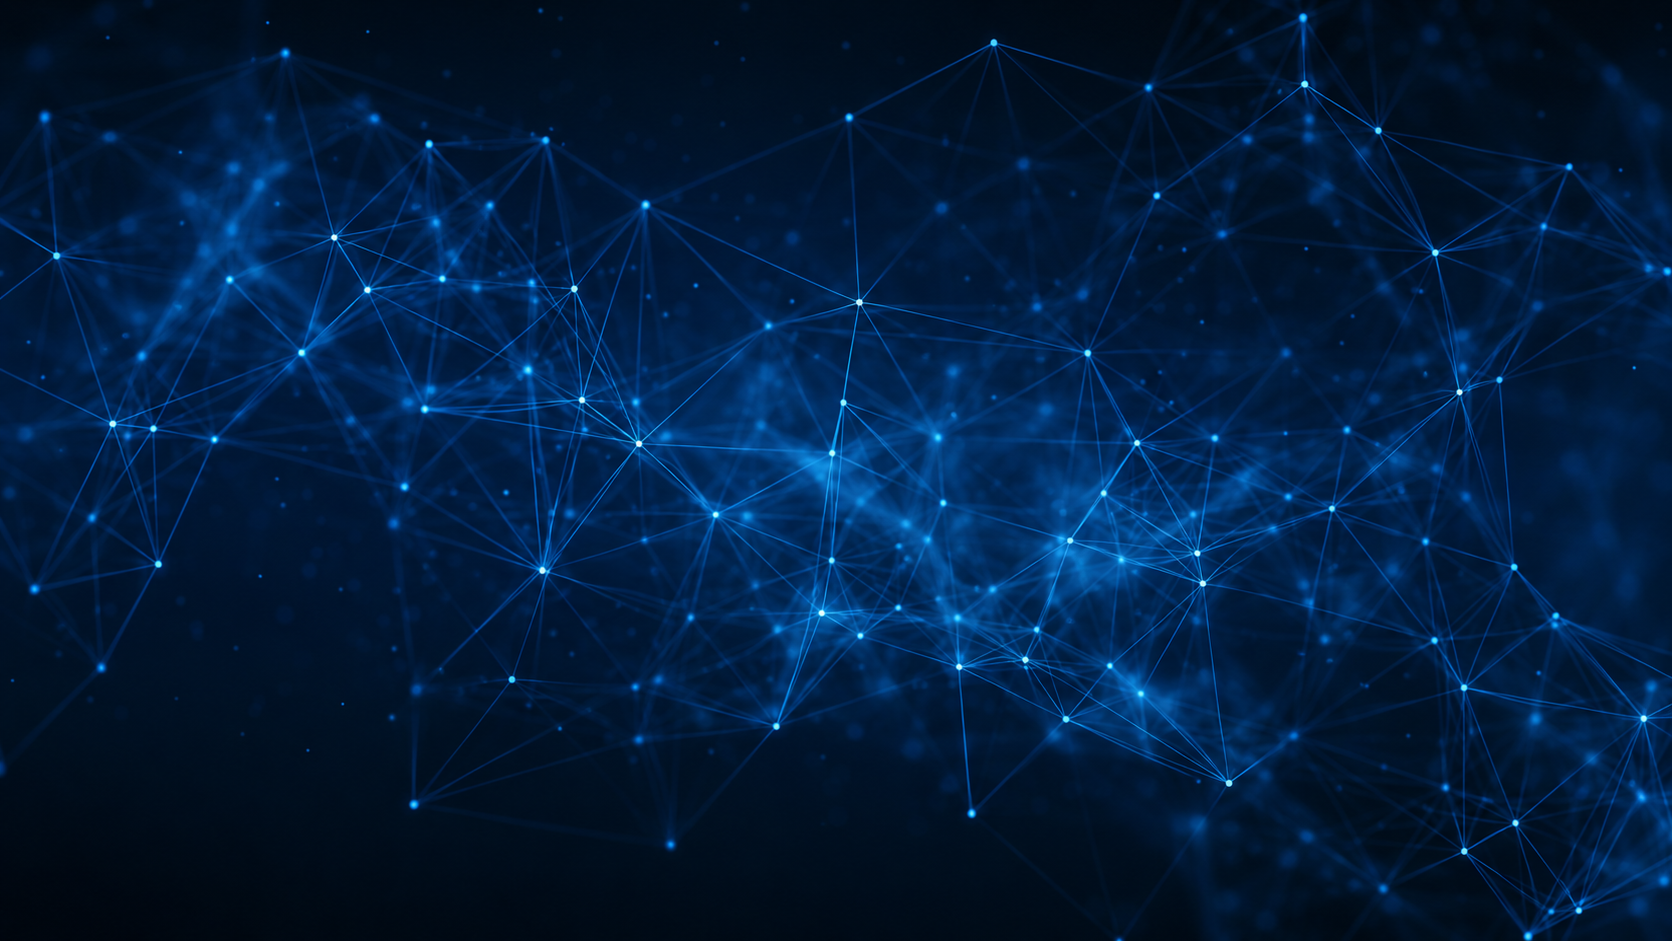
\includegraphics[width=\paperwidth, height=\paperheight]{121.png}
};
\fill[DarkBlue, opacity=0.72] (current page.south west) rectangle (current page.north east);

% Slide Number & Title
\node[anchor=west, text=TechYellow, font=\fontsize{14}{16}\selectfont\bfseries] at ([xshift=0.8cm,yshift=-0.65cm] current page.north west) {15};
\node[anchor=west, text=White, font=\fontsize{18}{22}\selectfont\bfseries] at ([xshift=1.8cm,yshift=-0.65cm] current page.north west) {Edge Computing and 5G};

% Pillar 1: 5G
\node[
    anchor=north west,
    draw=TechCyan,
    line width=0.8pt,
    rounded corners=6pt,
    fill=BoxTeal,
    fill opacity=0.95,
    text opacity=1,
    text width=6.6cm,
    minimum height=2.00cm,
    inner xsep=0.25cm,
    inner ysep=0.15cm
]
at ([xshift=0.8cm,yshift=-1.15cm] current page.north west)
{
    \textcolor{TechCyan}{\fontsize{10.5}{13}\selectfont\bfseries 5G Infrastructure}\\[3pt]
    \textcolor{SoftWhite}{\fontsize{8.5}{11.5}\selectfont High Bandwidth $+$ Ultra-Low Latency Connectivity}
};

% Pillar 2: Edge
\node[
    anchor=north west,
    draw=TechYellow,
    line width=0.8pt,
    rounded corners=6pt,
    fill=BoxPurple,
    fill opacity=0.95,
    text opacity=1,
    text width=6.6cm,
    minimum height=2.00cm,
    inner xsep=0.25cm,
    inner ysep=0.15cm
]
at ([xshift=8.2cm,yshift=-1.15cm] current page.north west)
{
    \textcolor{TechYellow}{\fontsize{10.5}{13}\selectfont\bfseries Edge Infrastructure}\\[3pt]
    \textcolor{SoftWhite}{\fontsize{8.5}{11.5}\selectfont Nearby Compute Node $+$ On-Site Data Processing}
};

% Middle Synergy Box
\node[
    anchor=north west,
    draw=TechYellow,
    line width=0.8pt,
    rounded corners=6pt,
    fill=BoxSlate,
    fill opacity=0.95,
    text opacity=1,
    text width=14.0cm,
    minimum height=3.30cm,
    inner xsep=0.30cm,
    inner ysep=0.18cm
]
at ([xshift=0.8cm,yshift=-3.40cm] current page.north west)
{
    \textcolor{TechYellow}{\fontsize{10.5}{13}\selectfont\bfseries Together, They Enable:}\\[6pt]
    \textcolor{SoftWhite}{\fontsize{8.5}{12}\selectfont
    \begin{tabular}{ll}
    \textcolor{TechCyan}{$\bullet$}\;\;\textcolor{White}{\bfseries Real-Time IoT Applications:} & Instant control loops for smart devices.\\[4pt]
    \textcolor{TechCyan}{$\bullet$}\;\;\textcolor{White}{\bfseries Local Video Analysis:} & Edge-based HD stream processing.\\[4pt]
    \textcolor{TechCyan}{$\bullet$}\;\;\textcolor{White}{\bfseries Location-Based Services:} & High-precision contextual data delivery.\\[4pt]
    \textcolor{TechCyan}{$\bullet$}\;\;\textcolor{White}{\bfseries Augmented Reality (AR):} & Lag-free immersive digital overlays.
    \end{tabular}
    }
};

% Key Idea Banner
\node[
    anchor=north west,
    draw=TechCyan,
    line width=0.8pt,
    rounded corners=6pt,
    fill=DarkBlue,
    fill opacity=0.95,
    text opacity=1,
    text width=14.0cm,
    align=center,
    inner xsep=0.20cm,
    inner ysep=0.16cm
]
at ([xshift=0.8cm,yshift=-7.00cm] current page.north west)
{
    \textcolor{TechYellow}{\fontsize{9.5}{12}\selectfont\bfseries Key Idea:}\;\;
    \textcolor{White}{\fontsize{9}{12}\selectfont
    \textbf{5G} provides fast connectivity; \textbf{Edge} provides nearby computation.
    }
};

\end{tikzpicture}

\end{frame}


% ==================================================
% SLIDE 16
% LIVE VIDEO BROADCASTING
% ==================================================

\begin{frame}[plain]

\begin{tikzpicture}[remember picture,overlay]

% Background
\node[anchor=south west, inner sep=0pt] at (current page.south west) {
    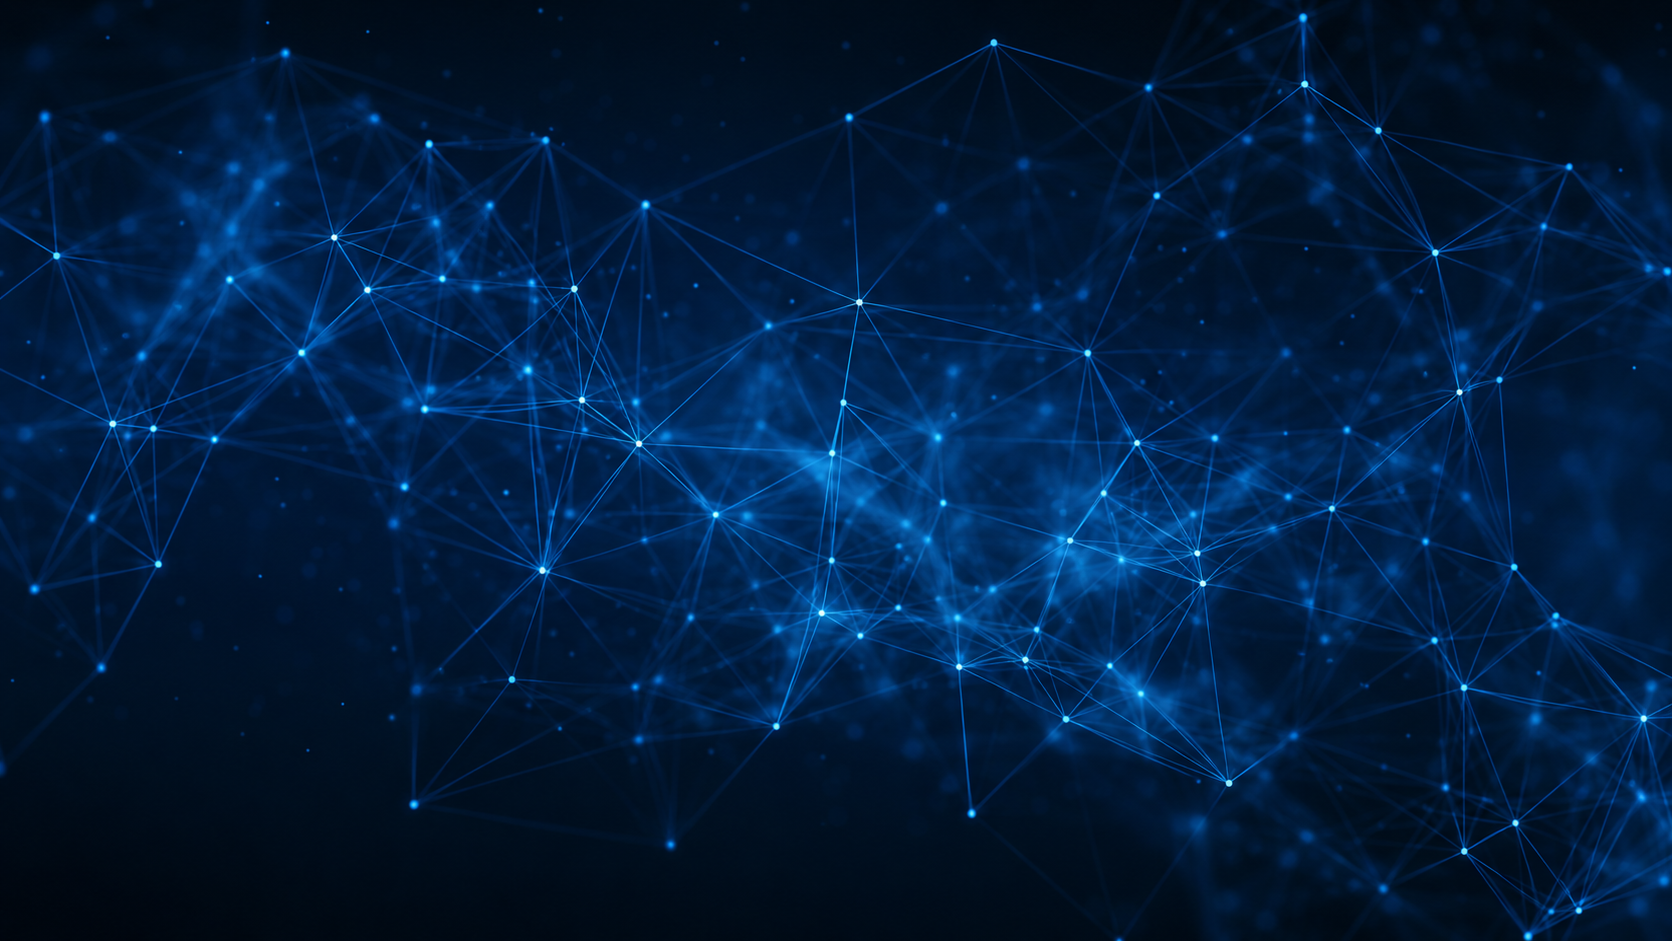
\includegraphics[width=\paperwidth, height=\paperheight]{121.png}
};
\fill[DarkBlue, opacity=0.72] (current page.south west) rectangle (current page.north east);

% Slide Number & Title
\node[anchor=west, text=TechYellow, font=\fontsize{14}{16}\selectfont\bfseries] at ([xshift=0.8cm,yshift=-0.65cm] current page.north west) {16};
\node[anchor=west, text=White, font=\fontsize{18}{22}\selectfont\bfseries] at ([xshift=1.8cm,yshift=-0.65cm] current page.north west) {Edge Computing for Live Video};

% Flow Banner
\node[
    anchor=north west,
    draw=TechCyan,
    line width=0.8pt,
    rounded corners=6pt,
    fill=DarkBlue,
    fill opacity=0.95,
    text opacity=1,
    text width=14.0cm,
    align=center,
    inner xsep=0.20cm,
    inner ysep=0.14cm
]
at ([xshift=0.8cm,yshift=-1.15cm] current page.north west)
{
    \textcolor{TechYellow}{\fontsize{9.5}{12}\selectfont\bfseries Broadcast Sequence:}\;\;
    \textcolor{White}{\fontsize{9}{12}\selectfont
    \textbf{Live Event} $\;\longrightarrow\;$ \textbf{\textcolor{TechCyan}{Edge Node}} $\;\longrightarrow\;$ \textbf{\textcolor{TechYellow}{Nearby Users}}
    }
};

% Left Card: Features
\node[
    anchor=north west,
    draw=TechCyan,
    line width=0.8pt,
    rounded corners=6pt,
    fill=BoxTeal,
    fill opacity=0.95,
    text opacity=1,
    text width=6.6cm,
    minimum height=5.30cm,
    inner xsep=0.25cm,
    inner ysep=0.18cm
]
at ([xshift=0.8cm,yshift=-2.15cm] current page.north west)
{
    \textcolor{TechCyan}{\fontsize{10.5}{13}\selectfont\bfseries Key Advantages}\\[6pt]
    \textcolor{TechCyan}{$\bullet$}\;\;\textcolor{White}{\bfseries Edge Transcoding:}\\[1.5pt]
    \hspace*{0.25cm}\textcolor{SoftWhite}{\fontsize{8.5}{11.5}\selectfont Video feeds are processed and stored at nearby edge nodes.}\\[5pt]
    \textcolor{TechCyan}{$\bullet$}\;\;\textcolor{White}{\bfseries Decoupled Cloud:}\\[1.5pt]
    \hspace*{0.25cm}\textcolor{SoftWhite}{\fontsize{8.5}{11.5}\selectfont Reduces reliance on centralized cloud servers.}\\[5pt]
    \textcolor{TechCyan}{$\bullet$}\;\;\textcolor{White}{\bfseries Ultra-Low Latency:}\\[1.5pt]
    \hspace*{0.25cm}\textcolor{SoftWhite}{\fontsize{8.5}{11.5}\selectfont Minimizes live streaming delay for audiences.}
};

% Right Card: Case Study
\node[
    anchor=north west,
    draw=TechYellow,
    line width=0.8pt,
    rounded corners=6pt,
    fill=BoxWine,
    fill opacity=0.95,
    text opacity=1,
    text width=6.6cm,
    minimum height=5.30cm,
    inner xsep=0.25cm,
    inner ysep=0.18cm
]
at ([xshift=8.2cm,yshift=-2.15cm] current page.north west)
{
    \textcolor{TechYellow}{\fontsize{10.5}{13}\selectfont\bfseries Case Study}\\[4pt]
    \textcolor{White}{\fontsize{9}{11}\selectfont\bfseries Shanghai Mercedes-Benz Cultural Center}\\[6pt]
    \textcolor{SoftWhite}{\fontsize{8.5}{11.5}\selectfont
    \textcolor{TechCyan}{$\bullet$}\;\;Deployed edge nodes directly inside the venue arena.\\[4pt]
    \textcolor{TechCyan}{$\bullet$}\;\;Achieved \textbf{millisecond-level latency} during multi-angle live event streaming.\\[4pt]
    \textcolor{TechCyan}{$\bullet$}\;\;Reported \textbf{more than $60\times$ lower latency} compared to conventional cloud broadcasting.
    }
};

\end{tikzpicture}

\end{frame}


% ==================================================
% SLIDE 17
% PREDICTIVE MAINTENANCE
% ==================================================

\begin{frame}[plain]

\begin{tikzpicture}[remember picture,overlay]

% Background
\node[anchor=south west, inner sep=0pt] at (current page.south west) {
    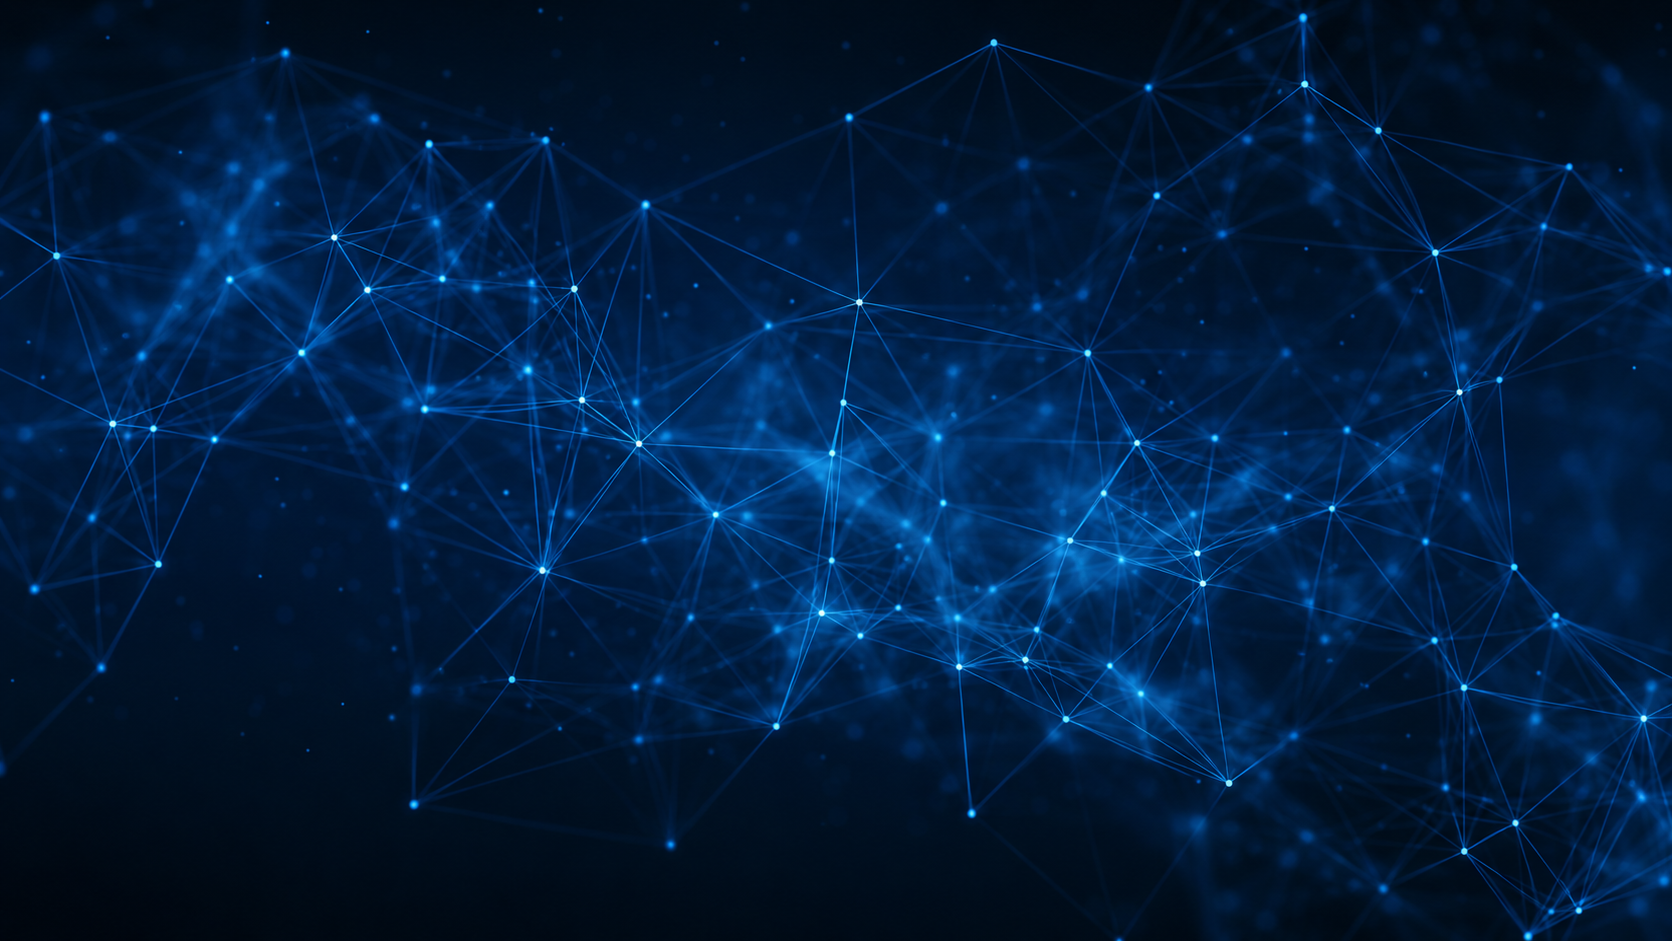
\includegraphics[width=\paperwidth, height=\paperheight]{121.png}
};
\fill[DarkBlue, opacity=0.72] (current page.south west) rectangle (current page.north east);

% Slide Number & Title
\node[anchor=west, text=TechYellow, font=\fontsize{14}{16}\selectfont\bfseries] at ([xshift=0.8cm,yshift=-0.65cm] current page.north west) {17};
\node[anchor=west, text=White, font=\fontsize{18}{22}\selectfont\bfseries] at ([xshift=1.8cm,yshift=-0.65cm] current page.north west) {Predictive Maintenance};

% Top Context Banner
\node[
    anchor=north west,
    draw=TechCyan,
    line width=0.8pt,
    rounded corners=6pt,
    fill=DarkBlue,
    fill opacity=0.95,
    text opacity=1,
    text width=14.0cm,
    align=center,
    inner xsep=0.20cm,
    inner ysep=0.12cm
]
at ([xshift=0.8cm,yshift=-1.15cm] current page.north west)
{
    \textcolor{SoftWhite}{\fontsize{8.5}{11.5}\selectfont
    Industrial machinery generates continuous high-frequency operational telemetry data.
    }
};

% Flow Banner
\node[
    anchor=north west,
    draw=TechYellow,
    line width=0.8pt,
    rounded corners=6pt,
    fill=DarkBlue,
    fill opacity=0.95,
    text opacity=1,
    text width=14.0cm,
    align=center,
    inner xsep=0.20cm,
    inner ysep=0.14cm
]
at ([xshift=0.8cm,yshift=-1.95cm] current page.north west)
{
    \textcolor{TechYellow}{\fontsize{9}{11}\selectfont\bfseries Process Sequence:}\;\;
    \textcolor{White}{\fontsize{8.5}{11}\selectfont
    \textbf{Equipment} $\;\longrightarrow\;$ \textbf{Sensors} $\;\longrightarrow\;$ \textbf{\textcolor{TechCyan}{Edge Processing}} $\;\longrightarrow\;$ \textbf{\textcolor{TechYellow}{Failure Prediction}}
    }
};

% Main Feature Box
\node[
    anchor=north west,
    draw=TechYellow,
    line width=0.8pt,
    rounded corners=6pt,
    fill=BoxEmerald,
    fill opacity=0.95,
    text opacity=1,
    text width=14.0cm,
    minimum height=3.60cm,
    inner xsep=0.30cm,
    inner ysep=0.18cm
]
at ([xshift=0.8cm,yshift=-2.95cm] current page.north west)
{
    \textcolor{TechYellow}{\fontsize{10.5}{13}\selectfont\bfseries Core Industrial Capabilities}\\[6pt]
    \textcolor{SoftWhite}{\fontsize{8.5}{12}\selectfont
    \textcolor{TechCyan}{$\bullet$}\;\;\textcolor{White}{\bfseries Continuous Monitoring:}\;\; Real-time tracking of vibration, temperature, and pressure.\\[4pt]
    \textcolor{TechCyan}{$\bullet$}\;\;\textcolor{White}{\bfseries Localized Data Analysis:}\;\; High-speed telemetry processed on-site without cloud delays.\\[4pt]
    \textcolor{TechCyan}{$\bullet$}\;\;\textcolor{White}{\bfseries Early Fault Detection:}\;\; Identifies subtle wear patterns to forecast machinery failures.\\[4pt]
    \textcolor{TechCyan}{$\bullet$}\;\;\textcolor{White}{\bfseries Industry 4.0 Foundation:}\;\; Enables fully autonomous and predictive smart factory operations.
    }
};

% Key Benefit Banner
\node[
    anchor=north west,
    draw=TechCyan,
    line width=0.8pt,
    rounded corners=6pt,
    fill=DarkBlue,
    fill opacity=0.95,
    text opacity=1,
    text width=14.0cm,
    align=center,
    inner xsep=0.20cm,
    inner ysep=0.16cm
]
at ([xshift=0.8cm,yshift=-6.95cm] current page.north west)
{
    \textcolor{TechYellow}{\fontsize{9.5}{12}\selectfont\bfseries Key Benefit:}\;\;
    \textcolor{White}{\fontsize{9}{12}\selectfont
    Detect and resolve problems \textbf{before} equipment failure causes costly downtime.
    }
};

\end{tikzpicture}

\end{frame}


% ==================================================
% SLIDE 18
% SECURITY MONITORING
% ==================================================

\begin{frame}[plain]

\begin{tikzpicture}[remember picture,overlay]

% Background
\node[anchor=south west, inner sep=0pt] at (current page.south west) {
    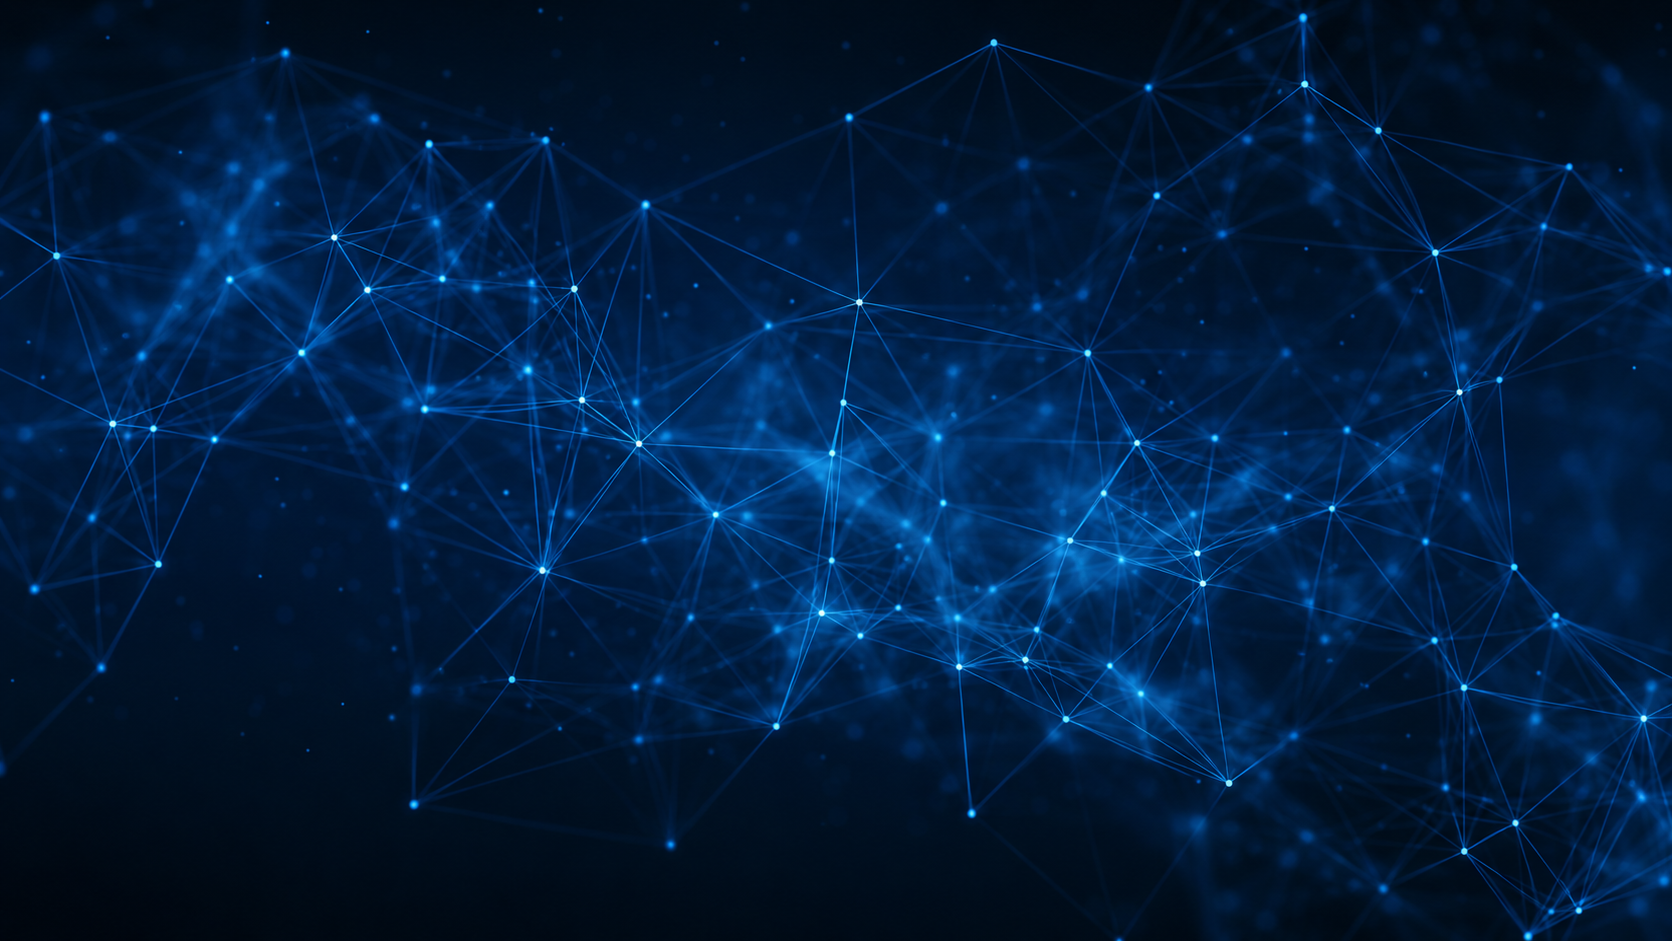
\includegraphics[width=\paperwidth, height=\paperheight]{121.png}
};
\fill[DarkBlue, opacity=0.72] (current page.south west) rectangle (current page.north east);

% Slide Number & Title
\node[anchor=west, text=TechYellow, font=\fontsize{14}{16}\selectfont\bfseries] at ([xshift=0.8cm,yshift=-0.65cm] current page.north west) {18};
\node[anchor=west, text=White, font=\fontsize{18}{22}\selectfont\bfseries] at ([xshift=1.8cm,yshift=-0.65cm] current page.north west) {Edge-Based Security Monitoring};

% Flow Banner
\node[
    anchor=north west,
    draw=TechCyan,
    line width=0.8pt,
    rounded corners=6pt,
    fill=DarkBlue,
    fill opacity=0.95,
    text opacity=1,
    text width=14.0cm,
    align=center,
    inner xsep=0.20cm,
    inner ysep=0.14cm
]
at ([xshift=0.8cm,yshift=-1.15cm] current page.north west)
{
    \textcolor{TechYellow}{\fontsize{9.5}{12}\selectfont\bfseries Monitoring Pipeline:}\;\;
    \textcolor{White}{\fontsize{9}{12}\selectfont
    \textbf{Camera} $\;\longrightarrow\;$ \textbf{\textcolor{TechCyan}{Edge Processing}} $\;\longrightarrow\;$ \textbf{Detection} $\;\longrightarrow\;$ \textbf{\textcolor{TechYellow}{Instant Alert}}
    }
};

% Left Card: Principles
\node[
    anchor=north west,
    draw=TechCyan,
    line width=0.8pt,
    rounded corners=6pt,
    fill=BoxPurple,
    fill opacity=0.95,
    text opacity=1,
    text width=7.4cm,
    minimum height=4.30cm,
    inner xsep=0.25cm,
    inner ysep=0.18cm
]
at ([xshift=0.8cm,yshift=-2.15cm] current page.north west)
{
    \textcolor{TechCyan}{\fontsize{10.5}{13}\selectfont\bfseries Edge Video Analytics}\\[6pt]
    \textcolor{TechCyan}{$\bullet$}\;\;\textcolor{White}{\bfseries Camera-Level AI:}\\[1.5pt]
    \hspace*{0.25cm}\textcolor{SoftWhite}{\fontsize{8.5}{11.5}\selectfont Video frames are analyzed locally at or near the camera.}\\[5pt]
    \textcolor{TechCyan}{$\bullet$}\;\;\textcolor{White}{\bfseries Instant Event Detection:}\\[1.5pt]
    \hspace*{0.25cm}\textcolor{SoftWhite}{\fontsize{8.5}{11.5}\selectfont Security triggers and anomalies are flagged immediately.}\\[5pt]
    \textcolor{TechCyan}{$\bullet$}\;\;\textcolor{White}{\bfseries Bandwidth Optimization:}\\[1.5pt]
    \hspace*{0.25cm}\textcolor{SoftWhite}{\fontsize{8.5}{11.5}\selectfont Avoids uploading continuous raw 24/7 video streams.}
};

% Right Card: Applications
\node[
    anchor=north west,
    draw=TechYellow,
    line width=0.8pt,
    rounded corners=6pt,
    fill=BoxSlate,
    fill opacity=0.95,
    text opacity=1,
    text width=5.8cm,
    minimum height=4.30cm,
    inner xsep=0.25cm,
    inner ysep=0.18cm
]
at ([xshift=9.0cm,yshift=-2.15cm] current page.north west)
{
    \textcolor{TechYellow}{\fontsize{10.5}{13}\selectfont\bfseries Target Applications}\\[6pt]
    \textcolor{TechYellow}{$\bullet$}\;\;\textcolor{White}{\bfseries Video Surveillance:}\\[1.5pt]
    \hspace*{0.25cm}\textcolor{SoftWhite}{\fontsize{8.5}{11.5}\selectfont Perimeter security enforcement.}\\[5pt]
    \textcolor{TechYellow}{$\bullet$}\;\;\textcolor{White}{\bfseries Pedestrian Recognition:}\\[1.5pt]
    \hspace*{0.25cm}\textcolor{SoftWhite}{\fontsize{8.5}{11.5}\selectfont Crowd density \& safety tracking.}\\[5pt]
    \textcolor{TechYellow}{$\bullet$}\;\;\textcolor{White}{\bfseries Abnormal Behavior:}\\[1.5pt]
    \hspace*{0.25cm}\textcolor{SoftWhite}{\fontsize{8.5}{11.5}\selectfont Intrusion \& hazard alerts.}
};

% Key Benefit Banner
\node[
    anchor=north west,
    draw=TechCyan,
    line width=0.8pt,
    rounded corners=6pt,
    fill=DarkBlue,
    fill opacity=0.95,
    text opacity=1,
    text width=14.0cm,
    align=center,
    inner xsep=0.20cm,
    inner ysep=0.16cm
]
at ([xshift=0.8cm,yshift=-6.80cm] current page.north west)
{
    \textcolor{TechYellow}{\fontsize{9.5}{12}\selectfont\bfseries Key Benefit:}\;\;
    \textcolor{White}{\fontsize{9}{12}\selectfont
    Real-time security monitoring with \textbf{significantly reduced network dependency}.
    }
};

\end{tikzpicture}

\end{frame}


% ==================================================
% SLIDE 19
% AUTONOMOUS VEHICLES
% ==================================================

\begin{frame}[plain]

\begin{tikzpicture}[remember picture,overlay]

% Background
\node[anchor=south west, inner sep=0pt] at (current page.south west) {
    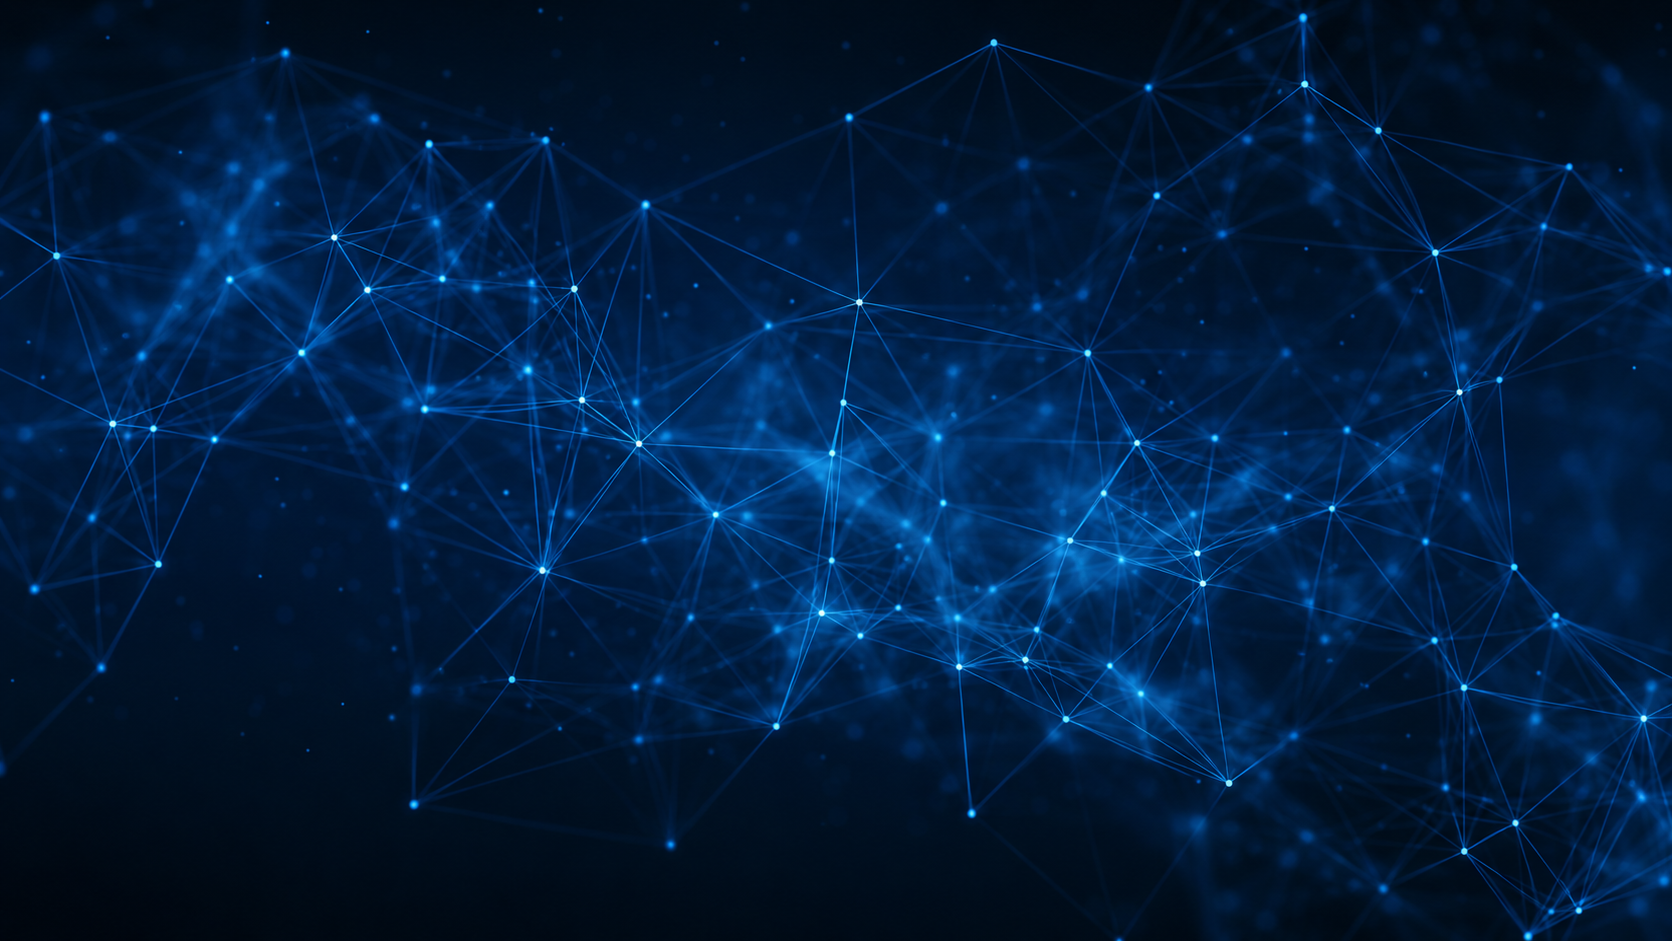
\includegraphics[width=\paperwidth, height=\paperheight]{121.png}
};
\fill[DarkBlue, opacity=0.72] (current page.south west) rectangle (current page.north east);

% Slide Number & Title
\node[anchor=west, text=TechYellow, font=\fontsize{14}{16}\selectfont\bfseries] at ([xshift=0.8cm,yshift=-0.65cm] current page.north west) {19};
\node[anchor=west, text=White, font=\fontsize{18}{22}\selectfont\bfseries] at ([xshift=1.8cm,yshift=-0.65cm] current page.north west) {Edge Computing in Autonomous Vehicles};

% Top Context Banner
\node[
    anchor=north west,
    draw=TechCyan,
    line width=0.8pt,
    rounded corners=6pt,
    fill=DarkBlue,
    fill opacity=0.95,
    text opacity=1,
    text width=14.0cm,
    align=center,
    inner xsep=0.20cm,
    inner ysep=0.12cm
]
at ([xshift=0.8cm,yshift=-1.15cm] current page.north west)
{
    \textcolor{SoftWhite}{\fontsize{8.5}{11.5}\selectfont
    Autonomous vehicles continuously process multi-sensor telemetry from cameras, Lidar, and Radar.
    }
};

% Flow Banner
\node[
    anchor=north west,
    draw=TechYellow,
    line width=0.8pt,
    rounded corners=6pt,
    fill=DarkBlue,
    fill opacity=0.95,
    text opacity=1,
    text width=14.0cm,
    align=center,
    inner xsep=0.20cm,
    inner ysep=0.14cm
]
at ([xshift=0.8cm,yshift=-1.95cm] current page.north west)
{
    \textcolor{TechYellow}{\fontsize{9}{11}\selectfont\bfseries Control Loop:}\;\;
    \textcolor{White}{\fontsize{8.5}{11}\selectfont
    \textbf{Sensors} $\;\longrightarrow\;$ \textbf{\textcolor{TechCyan}{Local Processing}} $\;\longrightarrow\;$ \textbf{Decision} $\;\longrightarrow\;$ \textbf{\textcolor{TechYellow}{Action}}
    }
};

% Left Card: Edge Capabilities
\node[
    anchor=north west,
    draw=TechCyan,
    line width=0.8pt,
    rounded corners=6pt,
    fill=BoxIndigo,
    fill opacity=0.95,
    text opacity=1,
    text width=6.6cm,
    minimum height=3.60cm,
    inner xsep=0.25cm,
    inner ysep=0.18cm
]
at ([xshift=0.8cm,yshift=-2.95cm] current page.north west)
{
    \textcolor{TechCyan}{\fontsize{10.5}{13}\selectfont\bfseries Onboard Edge Capabilities}\\[5pt]
    \textcolor{TechCyan}{$\bullet$}\;\;\textcolor{White}{\bfseries Real-Time Perception:}\\[1.5pt]
    \hspace*{0.25cm}\textcolor{SoftWhite}{\fontsize{8.5}{11.5}\selectfont Instant fusion of camera, Lidar, and Radar.}\\[4pt]
    \textcolor{TechCyan}{$\bullet$}\;\;\textcolor{White}{\bfseries Rapid Decision-Making:}\\[1.5pt]
    \hspace*{0.25cm}\textcolor{SoftWhite}{\fontsize{8.5}{11.5}\selectfont Sub-millisecond steering and throttle loop.}\\[4pt]
    \textcolor{TechCyan}{$\bullet$}\;\;\textcolor{White}{\bfseries Autonomous Offline Ops:}\\[1.5pt]
    \hspace*{0.25cm}\textcolor{SoftWhite}{\fontsize{8.5}{11.5}\selectfont Operates safely without cloud connectivity.}
};

% Right Card: Example Decisions
\node[
    anchor=north west,
    draw=TechYellow,
    line width=0.8pt,
    rounded corners=6pt,
    fill=BoxWine,
    fill opacity=0.95,
    text opacity=1,
    text width=6.6cm,
    minimum height=3.60cm,
    inner xsep=0.25cm,
    inner ysep=0.18cm
]
at ([xshift=8.2cm,yshift=-2.95cm] current page.north west)
{
    \textcolor{TechYellow}{\fontsize{10.5}{13}\selectfont\bfseries Example Control Decisions}\\[5pt]
    \textcolor{TechYellow}{$\bullet$}\;\;\textcolor{White}{\bfseries Obstacle Detection:}\\[1.5pt]
    \hspace*{0.25cm}\textcolor{SoftWhite}{\fontsize{8.5}{11.5}\selectfont Instant identification of hazards and vehicles.}\\[4pt]
    \textcolor{TechYellow}{$\bullet$}\;\;\textcolor{White}{\bfseries Lane Recognition:}\\[1.5pt]
    \hspace*{0.25cm}\textcolor{SoftWhite}{\fontsize{8.5}{11.5}\selectfont Precise path planning and lane keeping.}\\[4pt]
    \textcolor{TechYellow}{$\bullet$}\;\;\textcolor{White}{\bfseries Emergency Braking:}\\[1.5pt]
    \hspace*{0.25cm}\textcolor{SoftWhite}{\fontsize{8.5}{11.5}\selectfont Immediate collision avoidance action.}
};

% Key Requirement Banner
\node[
    anchor=north west,
    draw=TechCyan,
    line width=0.8pt,
    rounded corners=6pt,
    fill=DarkBlue,
    fill opacity=0.95,
    text opacity=1,
    text width=14.0cm,
    align=center,
    inner xsep=0.20cm,
    inner ysep=0.16cm
]
at ([xshift=0.8cm,yshift=-6.95cm] current page.north west)
{
    \textcolor{TechYellow}{\fontsize{9.5}{12}\selectfont\bfseries Key Requirement:}\;\;
    \textcolor{White}{\fontsize{9}{12}\selectfont
    Safety-critical decisions \textbf{must} be made within ultra-strict time constraints.
    }
};

\end{tikzpicture}

\end{frame}


% ==================================================
% SLIDE 20
% EDGE SCHEDULING (UNBOXED SLEEK TYPOGRAPHY LAYOUT)
% ==================================================

\begin{frame}[plain]

\begin{tikzpicture}[remember picture,overlay]

% Background
\node[anchor=south west, inner sep=0pt] at (current page.south west) {
    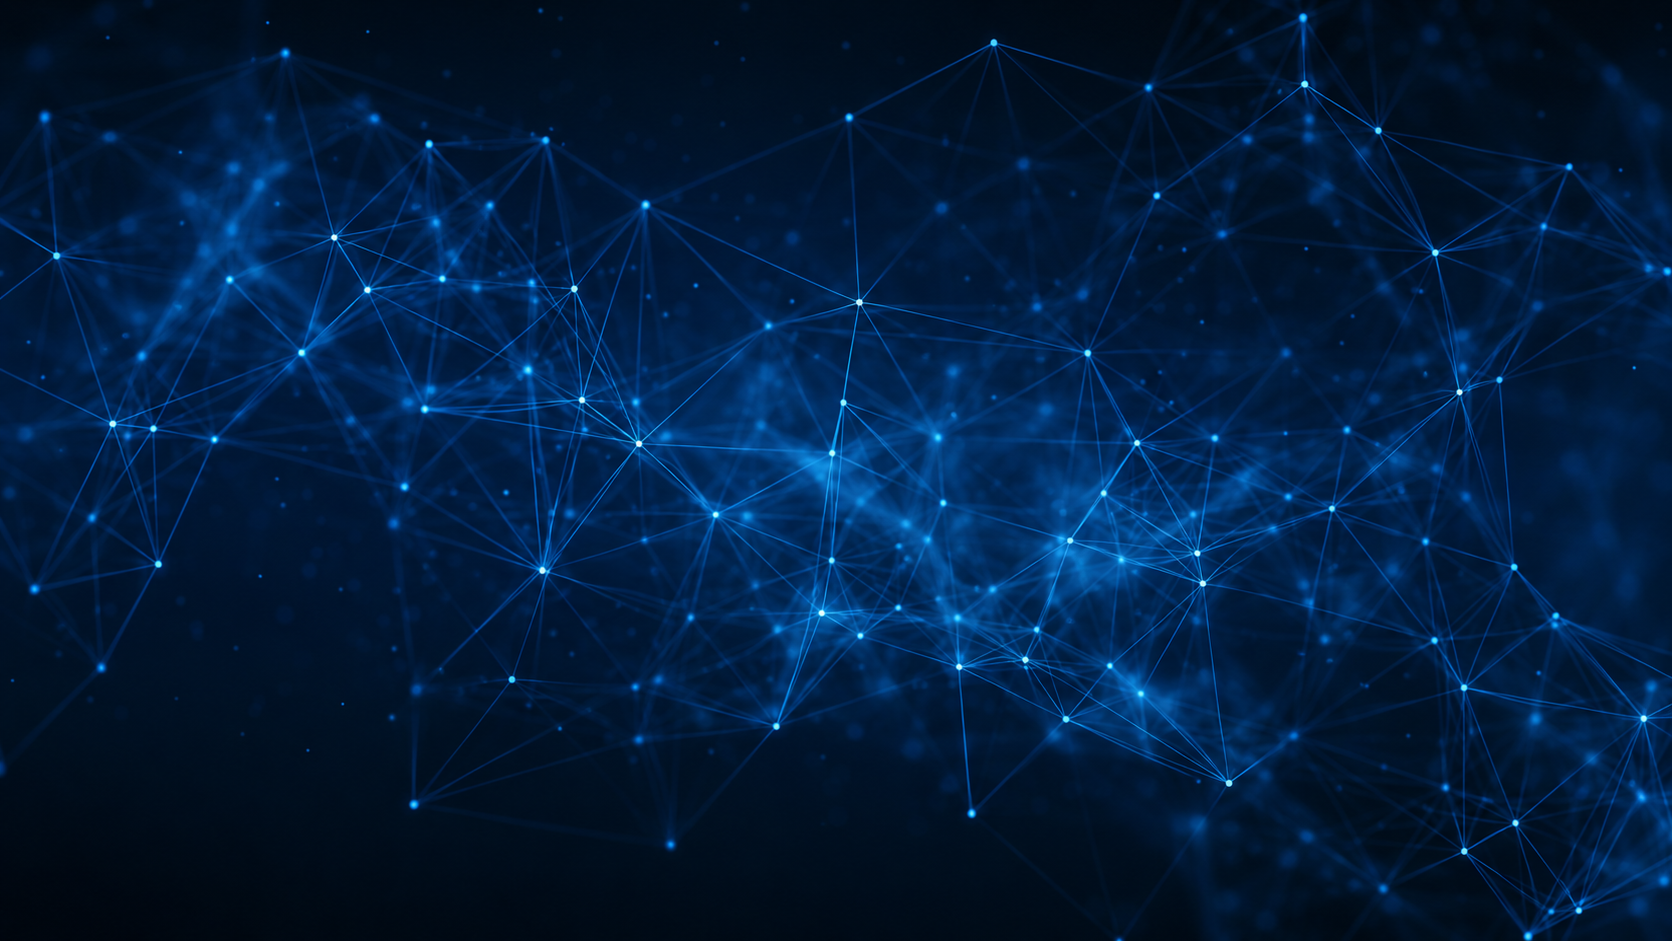
\includegraphics[width=\paperwidth, height=\paperheight]{121.png}
};
\fill[DarkBlue, opacity=0.72] (current page.south west) rectangle (current page.north east);

% Slide Number & Title
\node[anchor=west, text=TechYellow, font=\fontsize{14}{16}\selectfont\bfseries] at ([xshift=0.8cm,yshift=-0.65cm] current page.north west) {20};
\node[anchor=west, text=White, font=\fontsize{18}{22}\selectfont\bfseries] at ([xshift=1.8cm,yshift=-0.65cm] current page.north west) {Edge Scheduling};

% Top Definition Block (Unboxed)
\node[
    anchor=north west,
    text width=14.4cm,
    inner sep=0pt
]
at ([xshift=0.8cm,yshift=-1.15cm] current page.north west)
{
    \textcolor{TechYellow}{\fontsize{11}{13.5}\selectfont\bfseries Process Definition}\\[3pt]
    \textcolor{SoftWhite}{\fontsize{9}{12.5}\selectfont
    Edge Scheduling is the process of assigning incoming computational tasks to available edge resources while considering application deadlines, energy constraints, and system capabilities.
    }
};

% Top Horizontal Accent Line
\draw[TechCyan, line width=0.8pt, opacity=0.7]
    ([xshift=0.8cm,yshift=-2.65cm] current page.north west) --
    ([xshift=15.2cm,yshift=-2.65cm] current page.north west);

% Vertical Separator Line between columns
\draw[TechCyan!50!White, line width=0.6pt, opacity=0.4]
    ([xshift=7.8cm,yshift=-2.85cm] current page.north west) --
    ([xshift=7.8cm,yshift=-6.70cm] current page.north west);

% Column 1: Core Function & Primary Goal (Unboxed)
\node[
    anchor=north west,
    text width=6.6cm,
    inner sep=0pt
]
at ([xshift=0.8cm,yshift=-2.85cm] current page.north west)
{
    \textcolor{TechYellow}{\fontsize{10.5}{13}\selectfont\bfseries 01 \quad Core Functions}\\[5pt]
    \textcolor{TechCyan}{$\bullet$}\;\;\textcolor{White}{\bfseries Execution Control:}\\[1.5pt]
    \hspace*{0.25cm}\textcolor{SoftWhite}{\fontsize{8.5}{11.5}\selectfont Decides \textbf{where, when, and how} computing tasks run across terminals, edge nodes, and cloud.}\\[5pt]
    \textcolor{TechCyan}{$\bullet$}\;\;\textcolor{White}{\bfseries Primary Goal:}\\[1.5pt]
    \hspace*{0.25cm}\textcolor{SoftWhite}{\fontsize{8.5}{11.5}\selectfont Match each task to the resource meeting its \textbf{latency, energy, and accuracy} needs --- without overloading any node.}
};

% Column 2: Scheduling vs. Offloading (Unboxed)
\node[
    anchor=north west,
    text width=6.7cm,
    inner sep=0pt
]
at ([xshift=8.3cm,yshift=-2.85cm] current page.north west)
{
    \textcolor{TechCyan}{\fontsize{10.5}{13}\selectfont\bfseries 02 \quad Scheduling vs. Offloading}\\[5pt]
    \textcolor{TechCyan}{$\bullet$}\;\;\textcolor{White}{\bfseries Layered Architecture:}\\[1.5pt]
    \hspace*{0.25cm}\textcolor{SoftWhite}{\fontsize{8.5}{11.5}\selectfont Sits on top of computing offloading as an execution decision engine.}\\[5pt]
    \textcolor{TechCyan}{$\bullet$}\;\;\textcolor{White}{\bfseries Division of Labor:}\\[1.5pt]
    \hspace*{0.25cm}\textcolor{SoftWhite}{\fontsize{8.5}{11.5}\selectfont \textbf{Offloading} decides \textit{whether} to move a task; \textbf{Scheduling} decides \textit{which node} handles it and in what order.}
};

% Bottom Horizontal Accent Line
\draw[TechCyan, line width=0.8pt, opacity=0.7]
    ([xshift=0.8cm,yshift=-6.85cm] current page.north west) --
    ([xshift=15.2cm,yshift=-6.85cm] current page.north west);

% Bottom Summary Line (Unboxed)
\node[
    anchor=north west,
    text width=14.4cm,
    inner sep=0pt
]
at ([xshift=0.8cm,yshift=-7.12cm] current page.north west)
{
    \textcolor{TechYellow}{\fontsize{9.5}{12}\selectfont\bfseries Key Distinction:}\quad
    \textcolor{White}{\fontsize{8.5}{11.5}\selectfont
    \textbf{Offloading} $\rightarrow$ \textit{``Should we move it?''}
    \qquad\textcolor{TechCyan}{\textbf{|}}\qquad
    \textbf{Scheduling} $\rightarrow$ \textit{``Where and when does it run?''}
    }
};

\end{tikzpicture}

\end{frame}


% ==================================================
% SLIDE 21
% INTEGRATING REINFORCEMENT LEARNING
% ==================================================

\begin{frame}[plain]

\begin{tikzpicture}[remember picture,overlay]

% Background
\node[anchor=south west, inner sep=0pt] at (current page.south west) {
    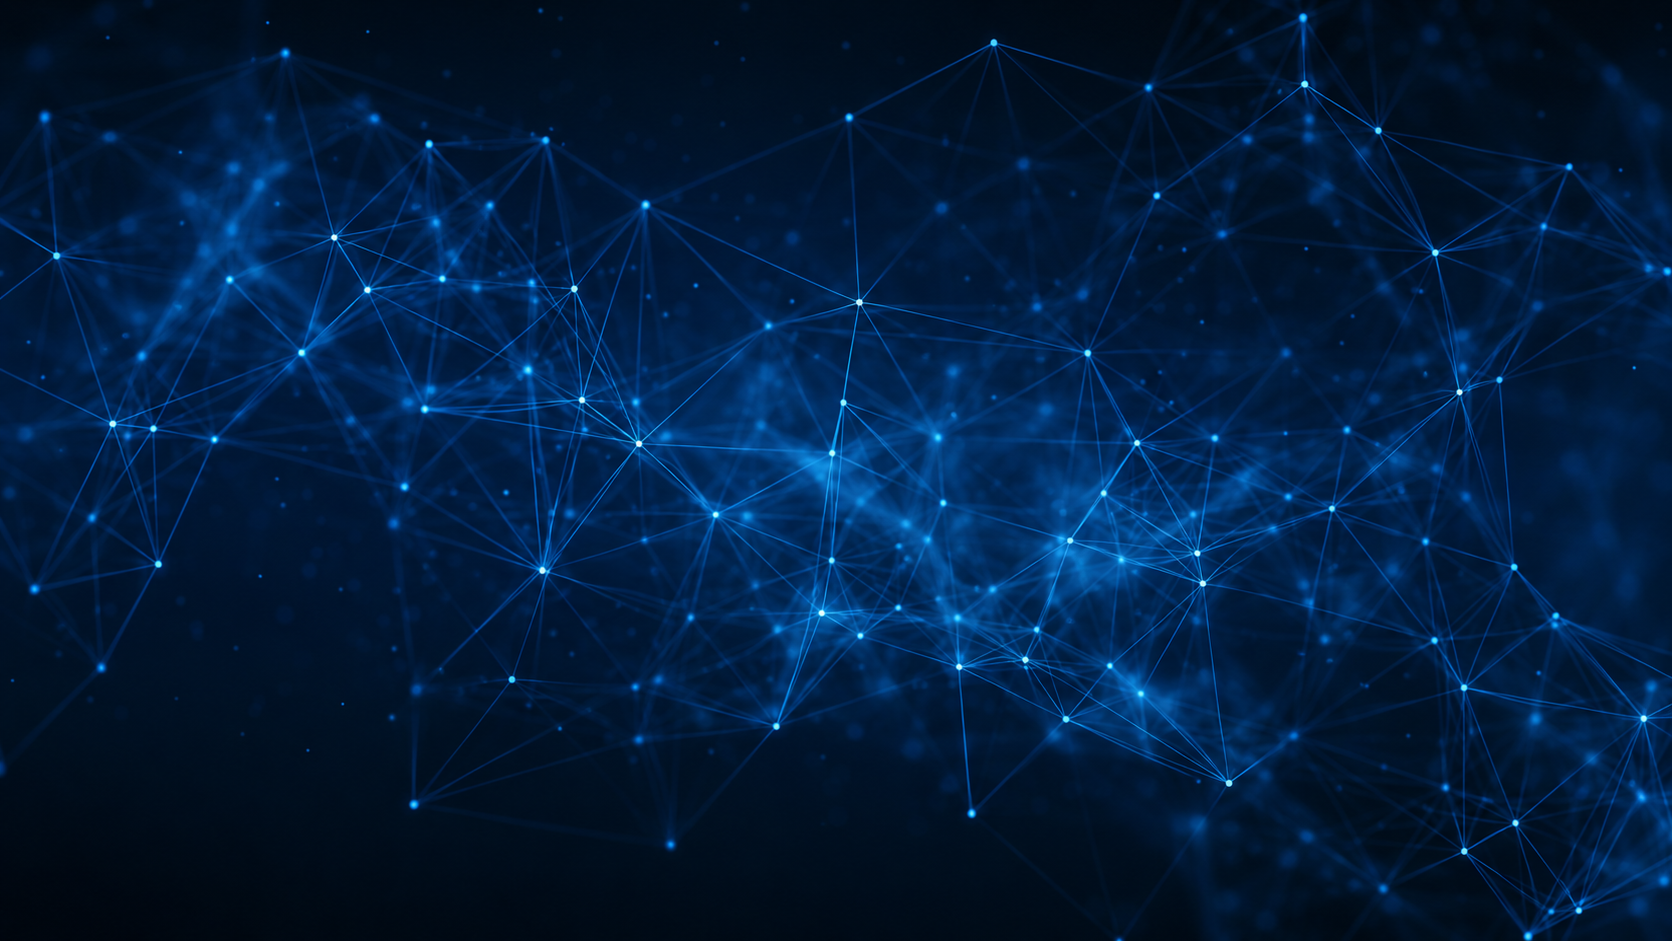
\includegraphics[width=\paperwidth, height=\paperheight]{121.png}
};
\fill[DarkBlue, opacity=0.72] (current page.south west) rectangle (current page.north east);

% Slide Number & Title
\node[anchor=west, text=TechYellow, font=\fontsize{14}{16}\selectfont\bfseries] at ([xshift=0.8cm,yshift=-0.65cm] current page.north west) {21};
\node[anchor=west, text=White, font=\fontsize{18}{22}\selectfont\bfseries] at ([xshift=1.8cm,yshift=-0.65cm] current page.north west) {Integrating Reinforcement Learning};

% Top Summary Block
\node[
    anchor=north west,
    text width=14.4cm,
    inner sep=0pt
]
at ([xshift=0.8cm,yshift=-1.10cm] current page.north west)
{
    \textcolor{SoftWhite}{\fontsize{8.2}{11}\selectfont
    Traditional scheduling approaches generally rely on \textbf{predefined rules, heuristics, or optimization procedures}.
    }\\[2.5pt]
    \textcolor{TechYellow}{\fontsize{8.5}{11.5}\selectfont\bfseries Why RL?}\;\;
    \textcolor{White}{\fontsize{8.2}{11}\selectfont
    Reinforcement Learning learns optimal policies by \textbf{interacting with the dynamic edge environment}.
    }
};

% Embedded Image Diagram Container (RL model.png)
\node[
    anchor=north west,
    draw=TechCyan,
    line width=0.8pt,
    rounded corners=6pt,
    fill=White,
    fill opacity=1,
    text opacity=1,
    inner sep=0.08cm
]
at ([xshift=0.8cm,yshift=-2.15cm] current page.north west)
{
    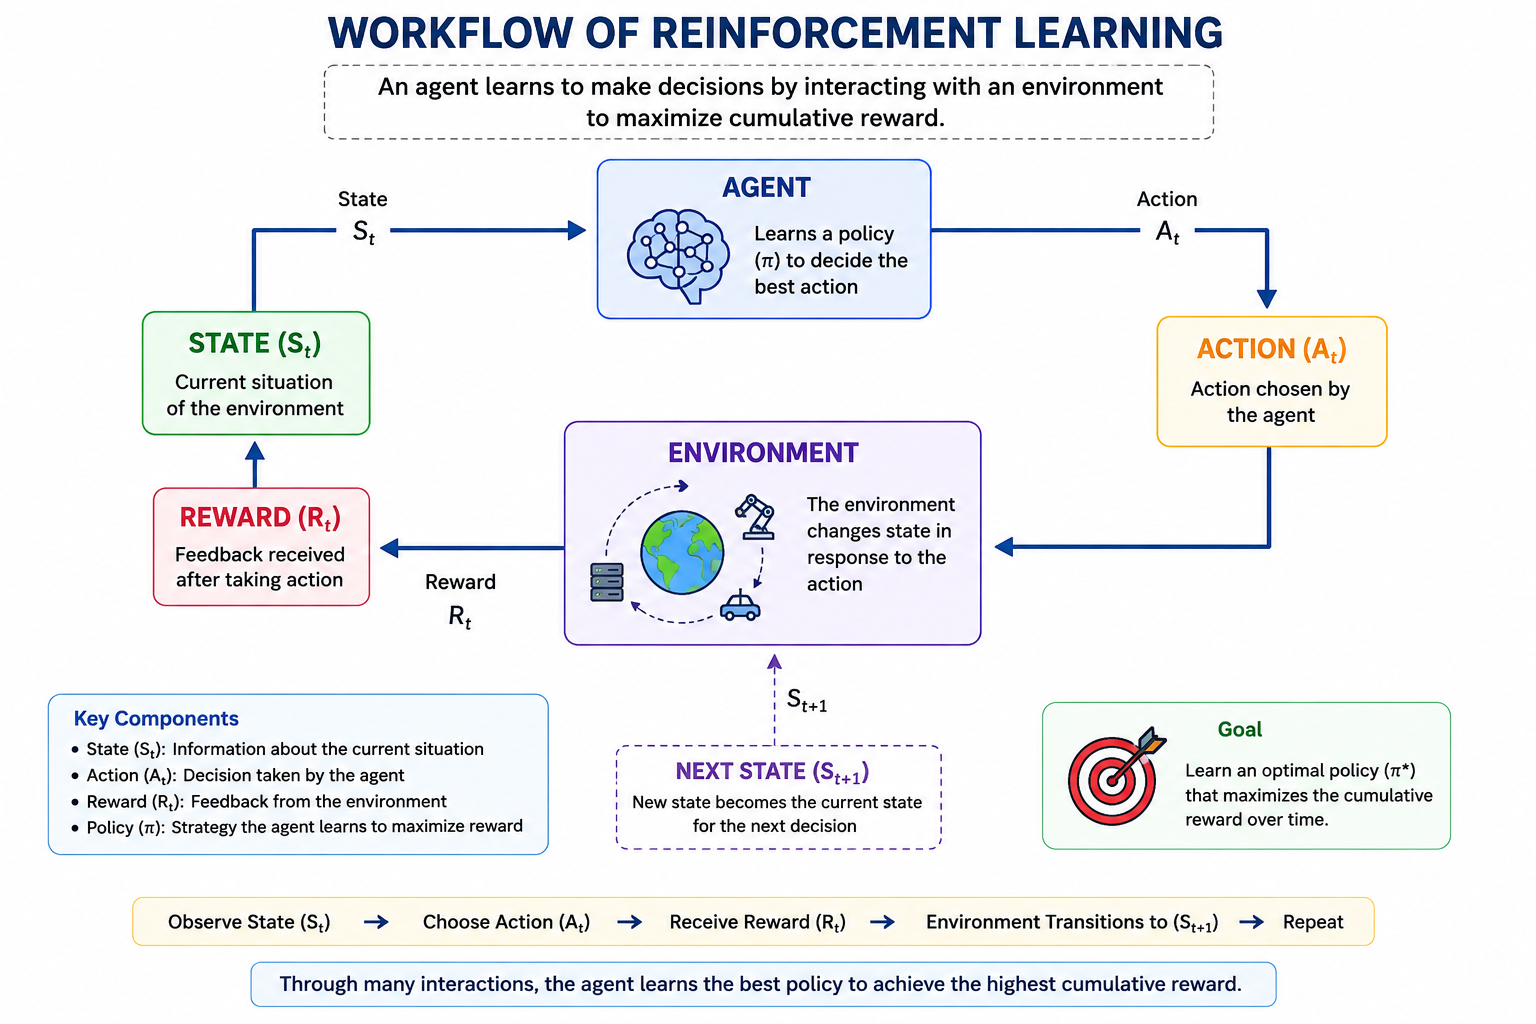
\includegraphics[width=14.4cm, height=5.15cm, keepaspectratio]{rl_model_pic.png}
};

\end{tikzpicture}

\end{frame}


% ==================================================
% SLIDE 22
% RL-BASED EDGE SCHEDULING WORKFLOW
% ==================================================

\begin{frame}[plain]

\begin{tikzpicture}[remember picture,overlay]

% Background
\node[anchor=south west, inner sep=0pt] at (current page.south west) {
    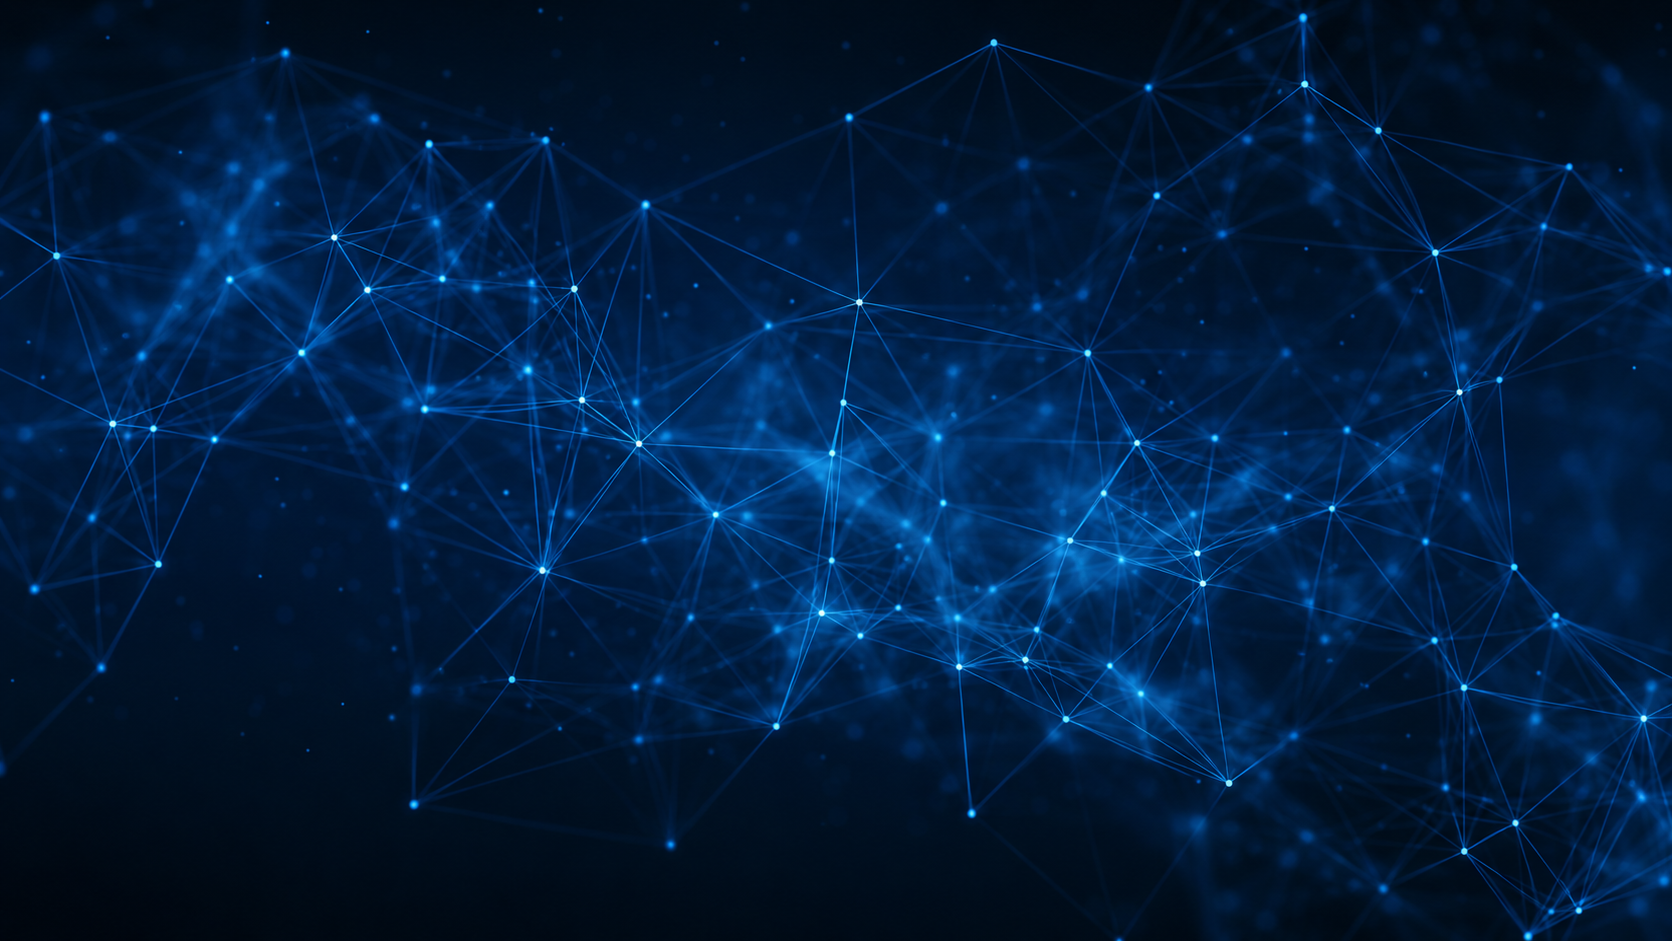
\includegraphics[width=\paperwidth, height=\paperheight]{121.png}
};
\fill[DarkBlue, opacity=0.72] (current page.south west) rectangle (current page.north east);

% Slide Number & Title
\node[anchor=west, text=TechYellow, font=\fontsize{14}{16}\selectfont\bfseries] at ([xshift=0.8cm,yshift=-0.65cm] current page.north west) {22};
\node[anchor=west, text=White, font=\fontsize{18}{22}\selectfont\bfseries] at ([xshift=1.8cm,yshift=-0.65cm] current page.north west) {RL-Based Edge Scheduling Workflow};

% Workflow Infographic Image
\node[
    anchor=north west,
    inner sep=0pt
]
at ([xshift=0.8cm,yshift=-1.15cm] current page.north west)
{
    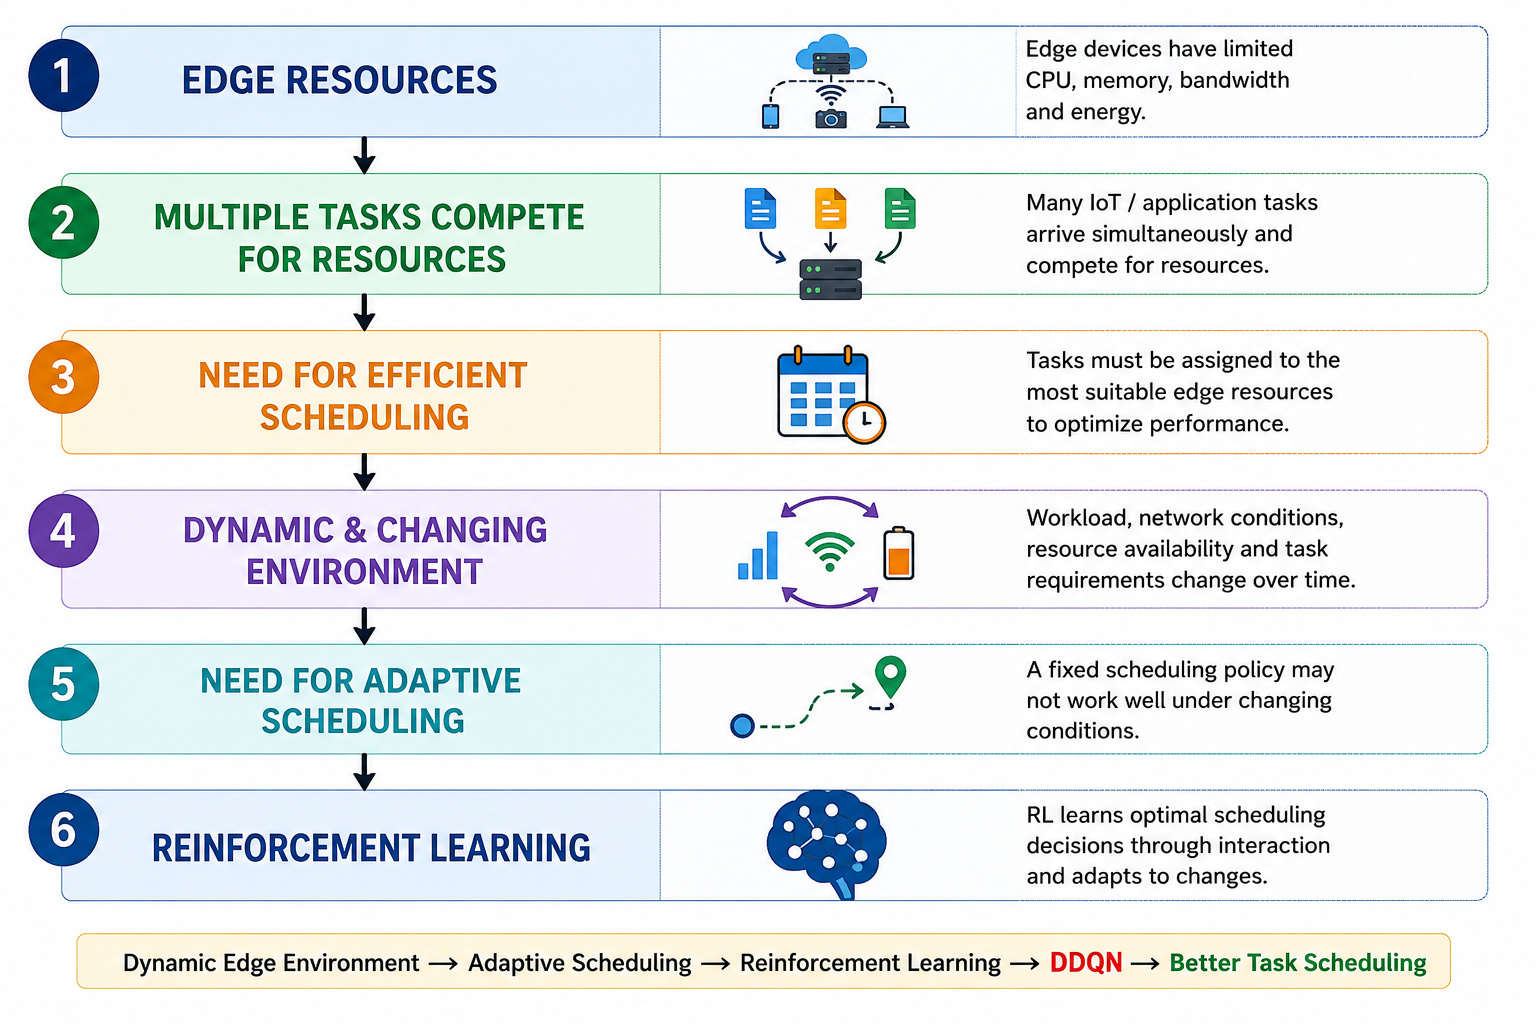
\includegraphics[width=14.4cm, height=6.3cm]{rl_edge_workflow_infographic.png}
};

\end{tikzpicture}

\end{frame}


% ==================================================
% SLIDE 23
% REAL-WORLD CASE STUDIES IN EDGE COMPUTING
% ==================================================
% SLIDE 23
% REAL-WORLD CASE STUDIES IN EDGE COMPUTING (WHITE CARDS)
% ==================================================

\begin{frame}[plain]

\begin{tikzpicture}[remember picture,overlay]

% Background
\node[anchor=south west, inner sep=0pt] at (current page.south west) {
    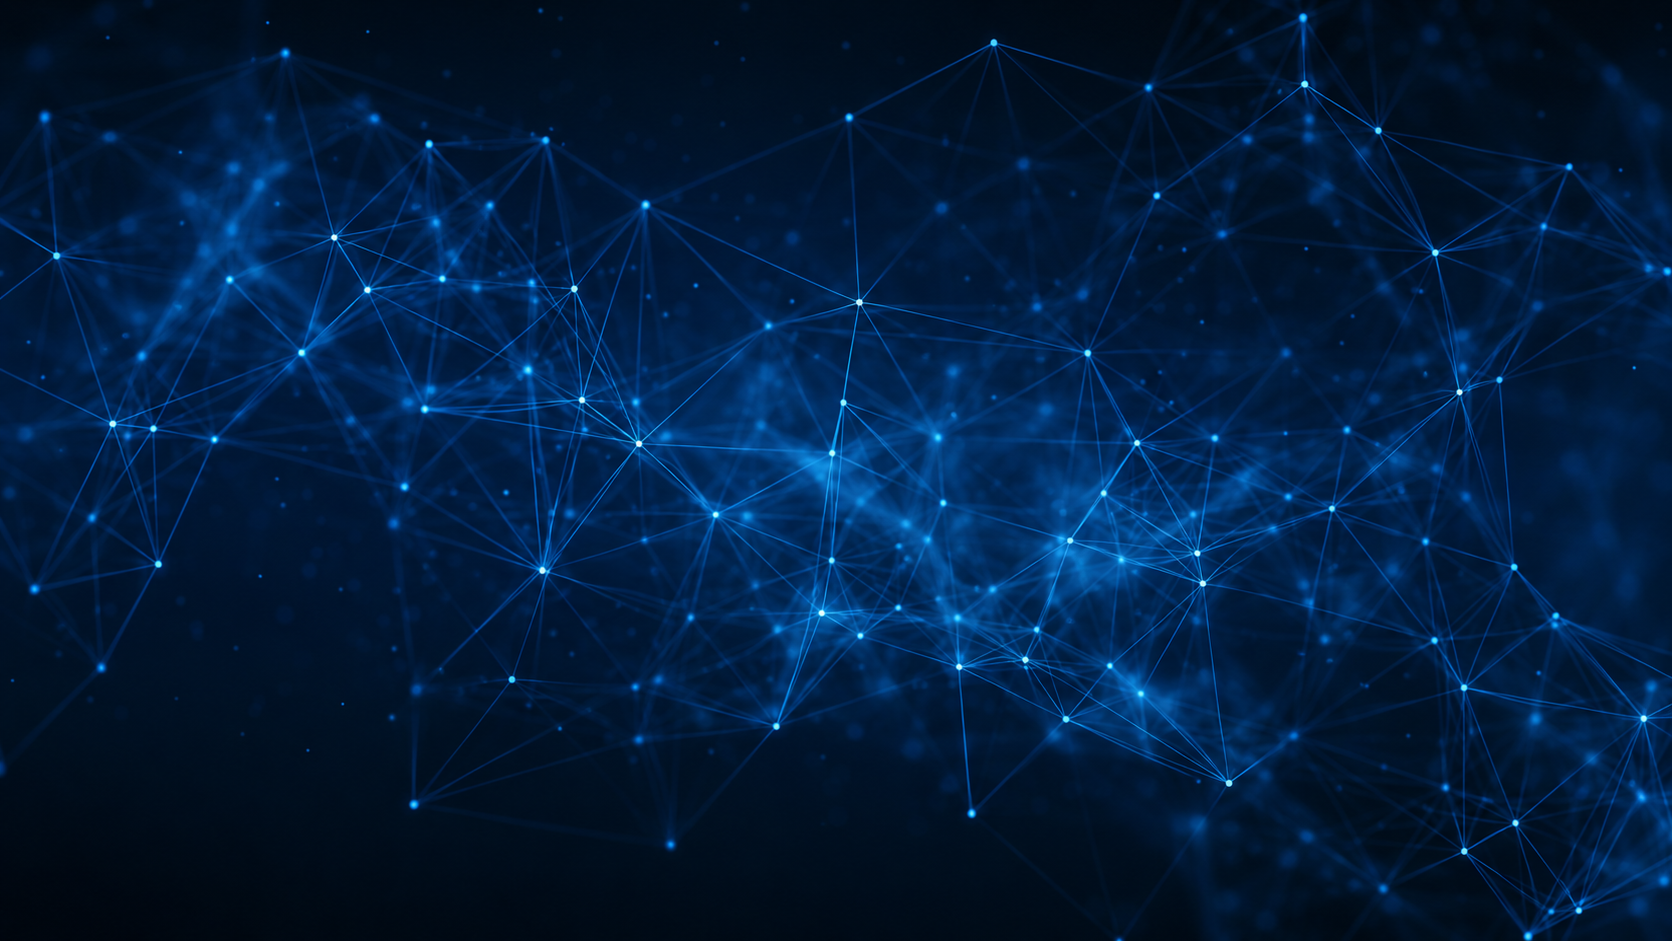
\includegraphics[width=\paperwidth, height=\paperheight]{121.png}
};
\fill[DarkBlue, opacity=0.72] (current page.south west) rectangle (current page.north east);

% Slide Number & Title
\node[anchor=west, text=TechYellow, font=\fontsize{14}{16}\selectfont\bfseries] at ([xshift=0.8cm,yshift=-0.65cm] current page.north west) {23};
\node[anchor=west, text=White, font=\fontsize{18}{22}\selectfont\bfseries] at ([xshift=1.8cm,yshift=-0.65cm] current page.north west) {Real-World Case Studies in Edge Computing};


% --------------------------------------------------
% ROW 1: 3 SEPARATED WHITE CARDS
% --------------------------------------------------

% Case Study 1: Autonomous Vehicles
\node[
    anchor=north west,
    draw=TechCyan,
    line width=0.8pt,
    rounded corners=6pt,
    fill=white,
    fill opacity=0.92,
    text opacity=1,
    text width=4.3cm,
    minimum height=2.50cm,
    inner xsep=0.18cm,
    inner ysep=0.10cm
]
at ([xshift=0.8cm,yshift=-1.20cm] current page.north west)
{
    \textcolor{DarkBlue}{\fontsize{9}{11.5}\selectfont\bfseries 01 Autonomous Vehicles}\\[2.5pt]
    \textcolor{darkgray}{\fontsize{7.2}{9.2}\selectfont
    Uses sensors, AI, and onboard compute to make driving decisions with little/no human intervention.
    }\\[3.5pt]
    \textcolor{BoxTeal}{\fontsize{7.2}{9.2}\selectfont\bfseries Why Edge?}\;\textcolor{darkgray}{\fontsize{7.2}{9.2}\selectfont Sub-ms latency for instant braking, steering \& obstacle avoidance.}
};

% Case Study 2: Smart Manufacturing
\node[
    anchor=north west,
    draw=TechYellow,
    line width=0.8pt,
    rounded corners=6pt,
    fill=white,
    fill opacity=0.92,
    text opacity=1,
    text width=4.3cm,
    minimum height=2.45cm,
    inner xsep=0.18cm,
    inner ysep=0.10cm
]
at ([xshift=5.6cm,yshift=-1.20cm] current page.north west)
{
    \textcolor{DarkBlue}{\fontsize{9}{11.5}\selectfont\bfseries 02 Smart Manufacturing}\\[2.5pt]
    \textcolor{darkgray}{\fontsize{7.2}{9.2}\selectfont
    Uses IoT sensors, machines, and AI to monitor and optimize factory production.
    }\\[3.5pt]
    \textcolor{BoxTeal}{\fontsize{7.2}{9.2}\selectfont\bfseries Why Edge?}\;\textcolor{darkgray}{\fontsize{7.2}{9.2}\selectfont Local sensor analysis for real-time fault detection.}
};

% Case Study 3: Smart Healthcare
\node[
    anchor=north west,
    draw=TechCyan,
    line width=0.8pt,
    rounded corners=6pt,
    fill=white,
    fill opacity=0.92,
    text opacity=1,
    text width=4.3cm,
    minimum height=2.45cm,
    inner xsep=0.18cm,
    inner ysep=0.10cm
]
at ([xshift=10.4cm,yshift=-1.20cm] current page.north west)
{
    \textcolor{DarkBlue}{\fontsize{9}{11.5}\selectfont\bfseries 03 Smart Healthcare}\\[2.5pt]
    \textcolor{darkgray}{\fontsize{7.2}{9.2}\selectfont
    Uses connected medical devices to continuously monitor patient vitals and support decisions.
    }\\[3.5pt]
    \textcolor{BoxTeal}{\fontsize{7.2}{9.2}\selectfont\bfseries Why Edge?}\;\textcolor{darkgray}{\fontsize{7.2}{9.2}\selectfont Rapid emergency alerts while preserving patient privacy.}
};


% --------------------------------------------------
% ROW 2: 2 SEPARATED WHITE CARDS
% --------------------------------------------------

% Case Study 4: Smart Agriculture
\node[
    anchor=north west,
    draw=TechYellow,
    line width=0.8pt,
    rounded corners=6pt,
    fill=white,
    fill opacity=0.92,
    text opacity=1,
    text width=6.6cm,
    minimum height=2.50cm,
    inner xsep=0.20cm,
    inner ysep=0.10cm
]
at ([xshift=0.8cm,yshift=-4.35cm] current page.north west)
{
    \textcolor{DarkBlue}{\fontsize{9}{11.5}\selectfont\bfseries 04 Smart Agriculture}\\[2.5pt]
    \textcolor{darkgray}{\fontsize{7.2}{9.2}\selectfont
    Uses IoT sensors, automation, and data analytics to monitor crops, soil, weather, and irrigation.
    }\\[3.5pt]
    \textcolor{BoxTeal}{\fontsize{7.2}{9.2}\selectfont\bfseries Why Edge?}\;\textcolor{darkgray}{\fontsize{7.2}{9.2}\selectfont Analyzes sensor data locally to trigger quick automated actions like irrigation.}
};

% Case Study 5: Intelligent Transportation System
\node[
    anchor=north west,
    draw=TechCyan,
    line width=0.8pt,
    rounded corners=6pt,
    fill=white,
    fill opacity=0.92,
    text opacity=1,
    text width=6.6cm,
    minimum height=2.50cm,
    inner xsep=0.20cm,
    inner ysep=0.10cm
]
at ([xshift=8.2cm,yshift=-4.35cm] current page.north west)
{
    \textcolor{DarkBlue}{\fontsize{9}{11.5}\selectfont\bfseries 05 Intelligent Transportation System (ITS)}\\[2.5pt]
    \textcolor{darkgray}{\fontsize{7.2}{9.2}\selectfont
    Uses roadside sensors, networks, and compute to monitor and manage city traffic flow.
    }\\[3.5pt]
    \textcolor{BoxTeal}{\fontsize{7.2}{9.2}\selectfont\bfseries Why Edge?}\;\textcolor{darkgray}{\fontsize{7.2}{9.2}\selectfont Local analysis for adaptive signals, congestion control \& accident detection.}
};

\end{tikzpicture}

\end{frame}


% ==================================================
% SLIDE 24
% CHALLENGES IN EDGE SCHEDULING -> POSSIBLE SOLUTIONS
% ==================================================

\begin{frame}[plain]

\begin{tikzpicture}[remember picture,overlay]

% Background
\node[anchor=south west, inner sep=0pt] at (current page.south west) {
    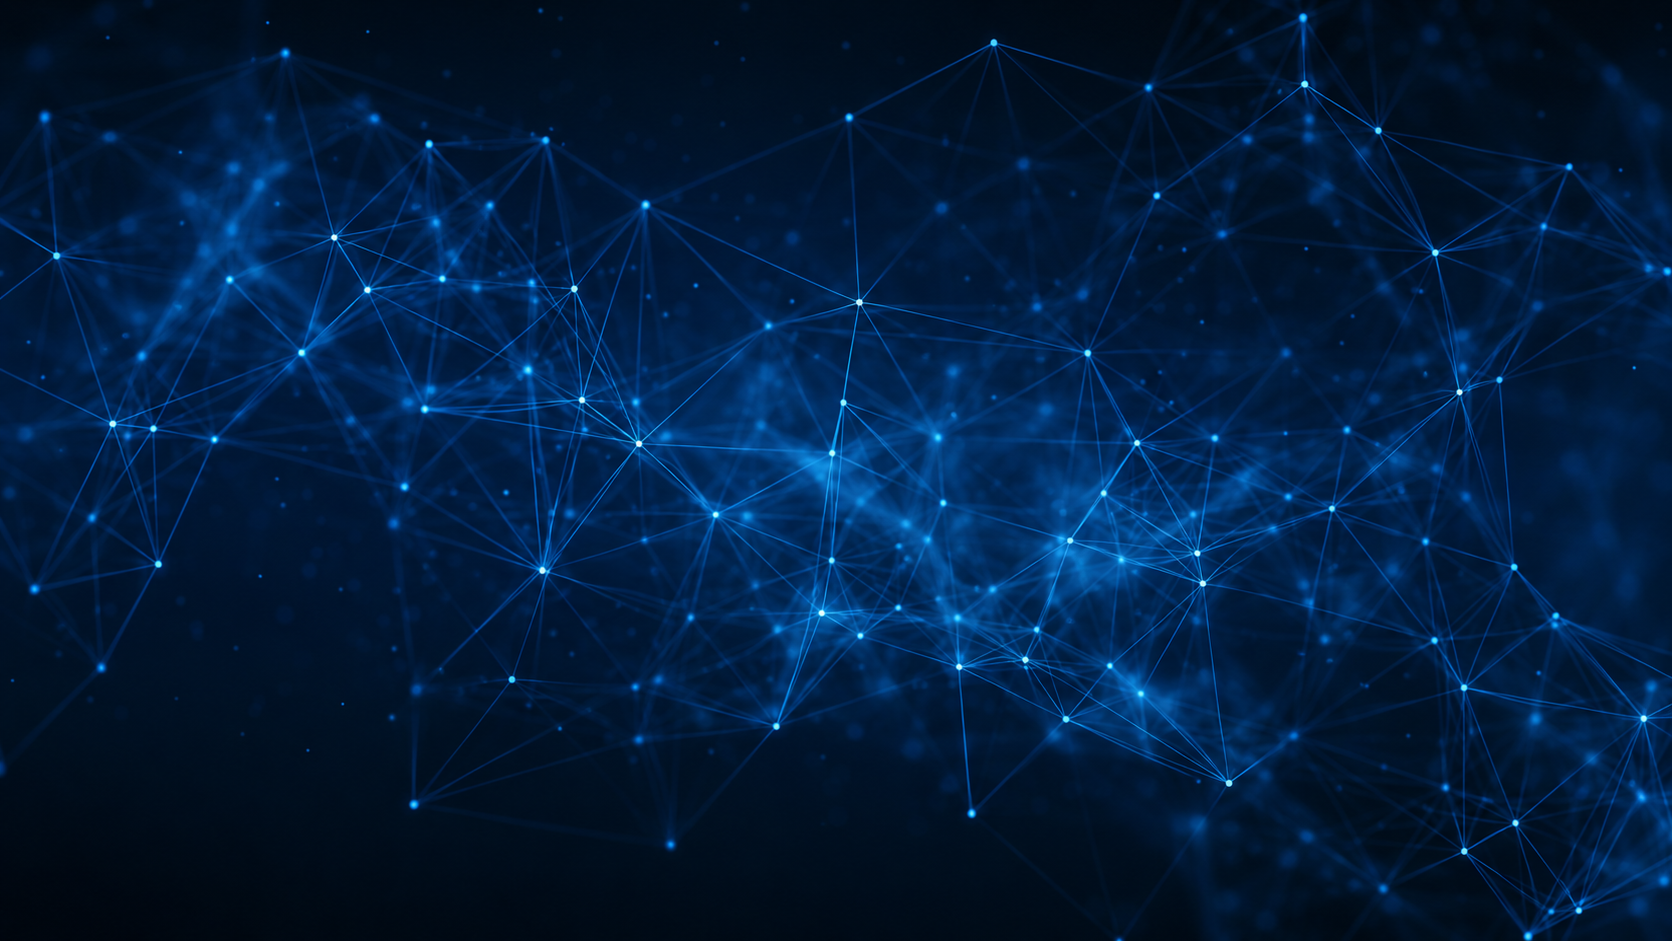
\includegraphics[width=\paperwidth, height=\paperheight]{121.png}
};
\fill[DarkBlue, opacity=0.72] (current page.south west) rectangle (current page.north east);

% Slide Number & Title
\node[anchor=west, text=TechYellow, font=\fontsize{14}{16}\selectfont\bfseries] at ([xshift=0.8cm,yshift=-0.65cm] current page.north west) {24};
\node[anchor=west, text=White, font=\fontsize{18}{22}\selectfont\bfseries] at ([xshift=1.8cm,yshift=-0.65cm] current page.north west) {Challenges in Edge Scheduling $\rightarrow$ Possible Solutions};

% --------------------------------------------------
% LEFT COLUMN: 4 CARDS
% --------------------------------------------------

% 01 Limited Resources
\node[
    anchor=north west,
    draw=TechCyan,
    line width=0.8pt,
    rounded corners=6pt,
    fill=white,
    fill opacity=0.92,
    text opacity=1,
    text width=6.6cm,
    minimum height=1.25cm,
    inner xsep=0.20cm,
    inner ysep=0.10cm
]
at ([xshift=0.8cm,yshift=-1.20cm] current page.north west)
{
    \textcolor{DarkBlue}{\fontsize{8.5}{11}\selectfont\bfseries Limited Resources}\\[2pt]
    \textcolor{BoxTeal}{\fontsize{7.5}{9.5}\selectfont\bfseries\(\rightarrow\)}\;\textcolor{darkgray}{\fontsize{7.5}{9.5}\selectfont Efficiently allocate CPU, memory, bandwidth, and energy.}
};

% 02 Dynamic Workloads
\node[
    anchor=north west,
    draw=TechYellow,
    line width=0.8pt,
    rounded corners=6pt,
    fill=white,
    fill opacity=0.92,
    text opacity=1,
    text width=6.6cm,
    minimum height=1.25cm,
    inner xsep=0.20cm,
    inner ysep=0.10cm
]
at ([xshift=0.8cm,yshift=-2.65cm] current page.north west)
{
    \textcolor{DarkBlue}{\fontsize{8.5}{11}\selectfont\bfseries Dynamic Workloads}\\[2pt]
    \textcolor{BoxTeal}{\fontsize{7.5}{9.5}\selectfont\bfseries\(\rightarrow\)}\;\textcolor{darkgray}{\fontsize{7.5}{9.5}\selectfont Continuously adapt scheduling decisions to changing task arrivals.}
};

% 03 Heterogeneous Devices
\node[
    anchor=north west,
    draw=TechCyan,
    line width=0.8pt,
    rounded corners=6pt,
    fill=white,
    fill opacity=0.92,
    text opacity=1,
    text width=6.6cm,
    minimum height=1.25cm,
    inner xsep=0.20cm,
    inner ysep=0.10cm
]
at ([xshift=0.8cm,yshift=-4.10cm] current page.north west)
{
    \textcolor{DarkBlue}{\fontsize{8.5}{11}\selectfont\bfseries Heterogeneous Devices}\\[2pt]
    \textcolor{BoxTeal}{\fontsize{7.5}{9.5}\selectfont\bfseries\(\rightarrow\)}\;\textcolor{darkgray}{\fontsize{7.5}{9.5}\selectfont Select resources based on their different capabilities.}
};

% 04 Network Latency
\node[
    anchor=north west,
    draw=TechYellow,
    line width=0.8pt,
    rounded corners=6pt,
    fill=white,
    fill opacity=0.92,
    text opacity=1,
    text width=6.6cm,
    minimum height=1.25cm,
    inner xsep=0.20cm,
    inner ysep=0.10cm
]
at ([xshift=0.8cm,yshift=-5.55cm] current page.north west)
{
    \textcolor{DarkBlue}{\fontsize{8.5}{11}\selectfont\bfseries Network Latency}\\[2pt]
    \textcolor{BoxTeal}{\fontsize{7.5}{9.5}\selectfont\bfseries\(\rightarrow\)}\;\textcolor{darkgray}{\fontsize{7.5}{9.5}\selectfont Schedule tasks closer to users to reduce communication delay.}
};


% --------------------------------------------------
% RIGHT COLUMN: 4 CARDS
% --------------------------------------------------

% 05 Energy Consumption
\node[
    anchor=north west,
    draw=TechYellow,
    line width=0.8pt,
    rounded corners=6pt,
    fill=white,
    fill opacity=0.92,
    text opacity=1,
    text width=6.6cm,
    minimum height=1.25cm,
    inner xsep=0.20cm,
    inner ysep=0.10cm
]
at ([xshift=8.2cm,yshift=-1.20cm] current page.north west)
{
    \textcolor{DarkBlue}{\fontsize{8.5}{11}\selectfont\bfseries Energy Consumption}\\[2pt]
    \textcolor{BoxTeal}{\fontsize{7.5}{9.5}\selectfont\bfseries\(\rightarrow\)}\;\textcolor{darkgray}{\fontsize{7.5}{9.5}\selectfont Include energy efficiency as a scheduling objective.}
};

% 06 Task Priorities
\node[
    anchor=north west,
    draw=TechCyan,
    line width=0.8pt,
    rounded corners=6pt,
    fill=white,
    fill opacity=0.92,
    text opacity=1,
    text width=6.6cm,
    minimum height=1.25cm,
    inner xsep=0.20cm,
    inner ysep=0.10cm
]
at ([xshift=8.2cm,yshift=-2.65cm] current page.north west)
{
    \textcolor{DarkBlue}{\fontsize{8.5}{11}\selectfont\bfseries Task Priorities}\\[2pt]
    \textcolor{BoxTeal}{\fontsize{7.5}{9.5}\selectfont\bfseries\(\rightarrow\)}\;\textcolor{darkgray}{\fontsize{7.5}{9.5}\selectfont Consider deadlines, QoS, and task importance.}
};

% 07 Scalability
\node[
    anchor=north west,
    draw=TechYellow,
    line width=0.8pt,
    rounded corners=6pt,
    fill=white,
    fill opacity=0.92,
    text opacity=1,
    text width=6.6cm,
    minimum height=1.25cm,
    inner xsep=0.20cm,
    inner ysep=0.10cm
]
at ([xshift=8.2cm,yshift=-4.10cm] current page.north west)
{
    \textcolor{DarkBlue}{\fontsize{8.5}{11}\selectfont\bfseries Scalability}\\[2pt]
    \textcolor{BoxTeal}{\fontsize{7.5}{9.5}\selectfont\bfseries\(\rightarrow\)}\;\textcolor{darkgray}{\fontsize{7.5}{9.5}\selectfont Use learning-based methods that handle many devices and tasks.}
};

% 08 Unpredictable Conditions
\node[
    anchor=north west,
    draw=TechCyan,
    line width=0.8pt,
    rounded corners=6pt,
    fill=white,
    fill opacity=0.92,
    text opacity=1,
    text width=6.6cm,
    minimum height=1.25cm,
    inner xsep=0.20cm,
    inner ysep=0.10cm
]
at ([xshift=8.2cm,yshift=-5.55cm] current page.north west)
{
    \textcolor{DarkBlue}{\fontsize{8.5}{11}\selectfont\bfseries Unpredictable Conditions}\\[2pt]
    \textcolor{BoxTeal}{\fontsize{7.5}{9.5}\selectfont\bfseries\(\rightarrow\)}\;\textcolor{darkgray}{\fontsize{7.5}{9.5}\selectfont Use Reinforcement Learning to learn and adapt scheduling policies.}
};

\end{tikzpicture}

\end{frame}


% ==================================================
% SLIDE 25
% SUMMARY (BULLETED LIST - UNBOXED)
% ==================================================

\begin{frame}[plain]

\begin{tikzpicture}[remember picture,overlay]

% Background
\node[anchor=south west, inner sep=0pt] at (current page.south west) {
    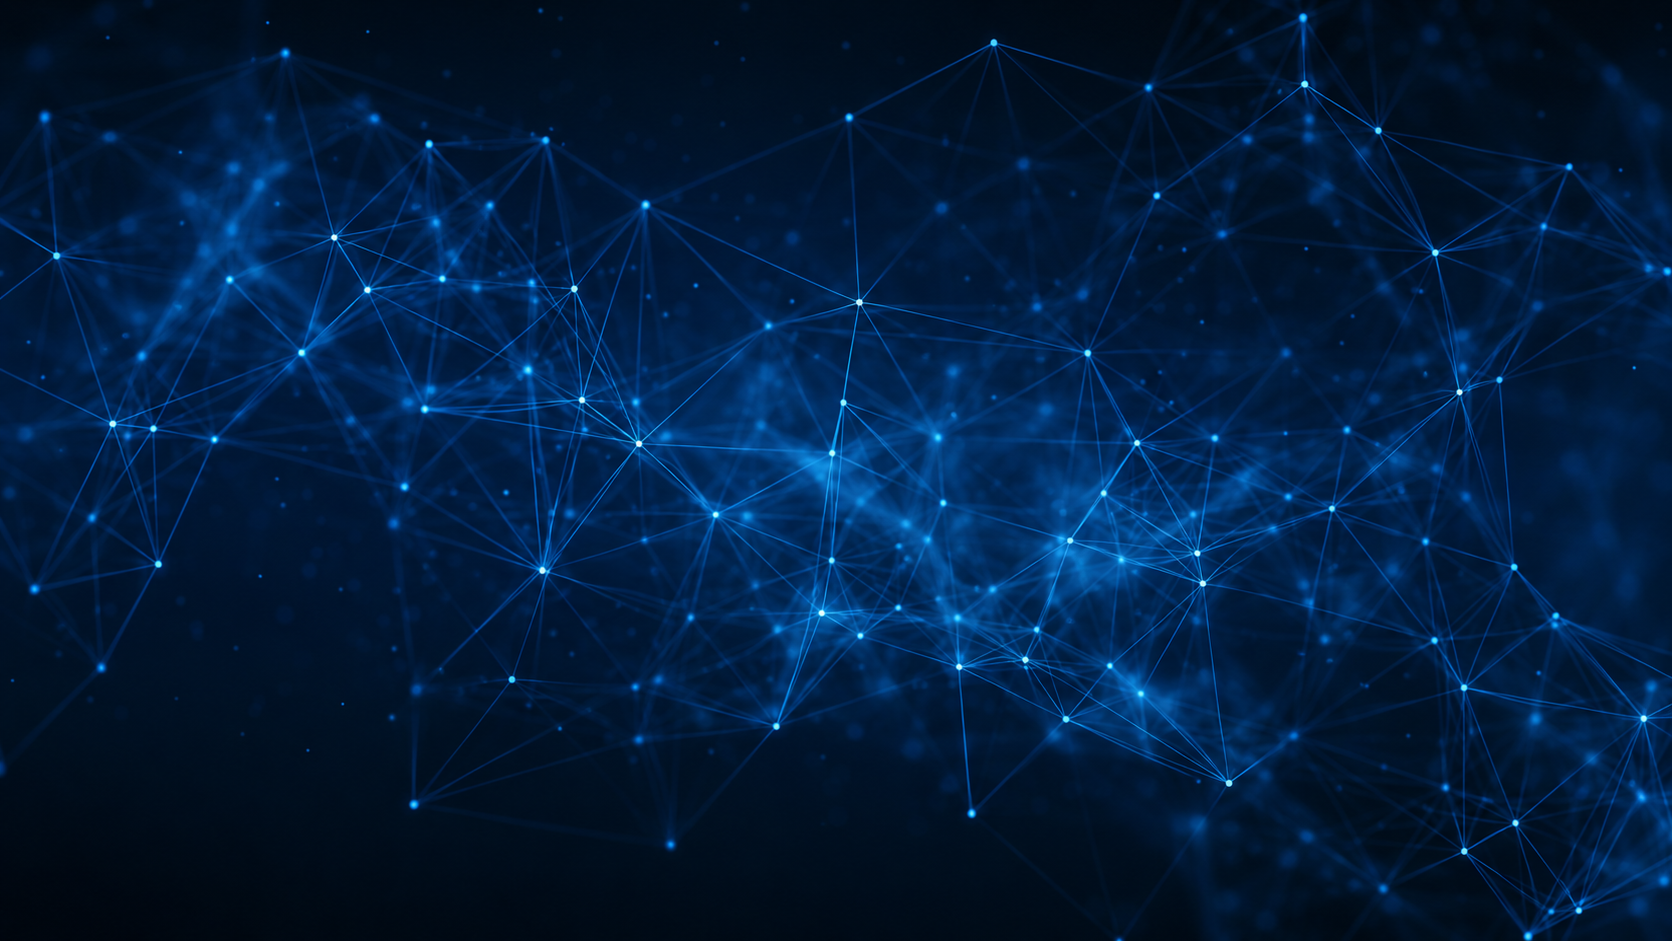
\includegraphics[width=\paperwidth, height=\paperheight]{121.png}
};
\fill[DarkBlue, opacity=0.72] (current page.south west) rectangle (current page.north east);

% Slide Number & Title
\node[anchor=west, text=TechYellow, font=\fontsize{14}{16}\selectfont\bfseries] at ([xshift=0.8cm,yshift=-0.65cm] current page.north west) {25};
\node[anchor=west, text=White, font=\fontsize{18}{22}\selectfont\bfseries] at ([xshift=1.8cm,yshift=-0.65cm] current page.north west) {Summary};

% Top Accent Divider Line
\draw[TechCyan, line width=0.8pt, opacity=0.6]
    ([xshift=0.8cm,yshift=-1.20cm] current page.north west) --
    ([xshift=15.2cm,yshift=-1.20cm] current page.north west);

% --------------------------------------------------
% BULLETED LIST (UNBOXED)
% --------------------------------------------------

% Bullet 1: Edge Computing & Constraints
\node[
    anchor=north west,
    text width=14.4cm,
    inner sep=0pt
]
at ([xshift=0.8cm,yshift=-1.50cm] current page.north west)
{
    \textcolor{TechYellow}{\fontsize{11}{14}\selectfont\bfseries\(\bullet\)}\;\;
    \textcolor{White}{\fontsize{9.5}{13.5}\selectfont
    \textbf{Edge Computing} brings computation closer to users, but edge devices have \textbf{limited resources}, \textbf{heterogeneous capabilities}, and \textbf{changing workloads}.
    }
};

% Bullet 2: Essential Task Scheduling
\node[
    anchor=north west,
    text width=14.4cm,
    inner sep=0pt
]
at ([xshift=0.8cm,yshift=-2.60cm] current page.north west)
{
    \textcolor{TechCyan}{\fontsize{11}{14}\selectfont\bfseries\(\bullet\)}\;\;
    \textcolor{White}{\fontsize{9.5}{13.5}\selectfont
    \textbf{Efficient scheduling} is essential to allocate tasks effectively and reduce \textbf{latency}, \textbf{energy consumption}, and \textbf{resource wastage}.
    }
};

% Bullet 3: Limitations of Traditional Fixed Methods
\node[
    anchor=north west,
    text width=14.4cm,
    inner sep=0pt
]
at ([xshift=0.8cm,yshift=-3.70cm] current page.north west)
{
    \textcolor{TechYellow}{\fontsize{11}{14}\selectfont\bfseries\(\bullet\)}\;\;
    \textcolor{White}{\fontsize{9.5}{13.5}\selectfont
    Since the edge environment is dynamic, \textbf{traditional fixed scheduling methods} may not always perform well.
    }
};

% Bullet 4: Reinforcement Learning Advantage
\node[
    anchor=north west,
    text width=14.4cm,
    inner sep=0pt
]
at ([xshift=0.8cm,yshift=-4.80cm] current page.north west)
{
    \textcolor{TechCyan}{\fontsize{11}{14}\selectfont\bfseries\(\bullet\)}\;\;
    \textcolor{White}{\fontsize{9.5}{13.5}\selectfont
    \textbf{Reinforcement Learning} can learn from the changing environment and make \textbf{adaptive scheduling decisions}.
    }
};

% Bullet 5: Advanced RL Techniques (DDQN)
\node[
    anchor=north west,
    text width=14.4cm,
    inner sep=0pt
]
at ([xshift=0.8cm,yshift=-5.90cm] current page.north west)
{
    \textcolor{TechYellow}{\fontsize{11}{14}\selectfont\bfseries\(\bullet\)}\;\;
    \textcolor{White}{\fontsize{9.5}{13.5}\selectfont
    Techniques such as \textbf{DDQN (Double Deep Q-Networks)} can further improve intelligent task scheduling in dynamic edge environments.
    }
};

% Bottom Accent Line
\draw[TechCyan, line width=0.8pt, opacity=0.6]
    ([xshift=0.8cm,yshift=-7.05cm] current page.north west) --
    ([xshift=15.2cm,yshift=-7.05cm] current page.north west);

\end{tikzpicture}

\end{frame}


% ==================================================
% SLIDE 26
% REFERENCES
% ==================================================

\begin{frame}[plain]

\begin{tikzpicture}[remember picture,overlay]

% Background
\node[anchor=south west, inner sep=0pt] at (current page.south west) {
    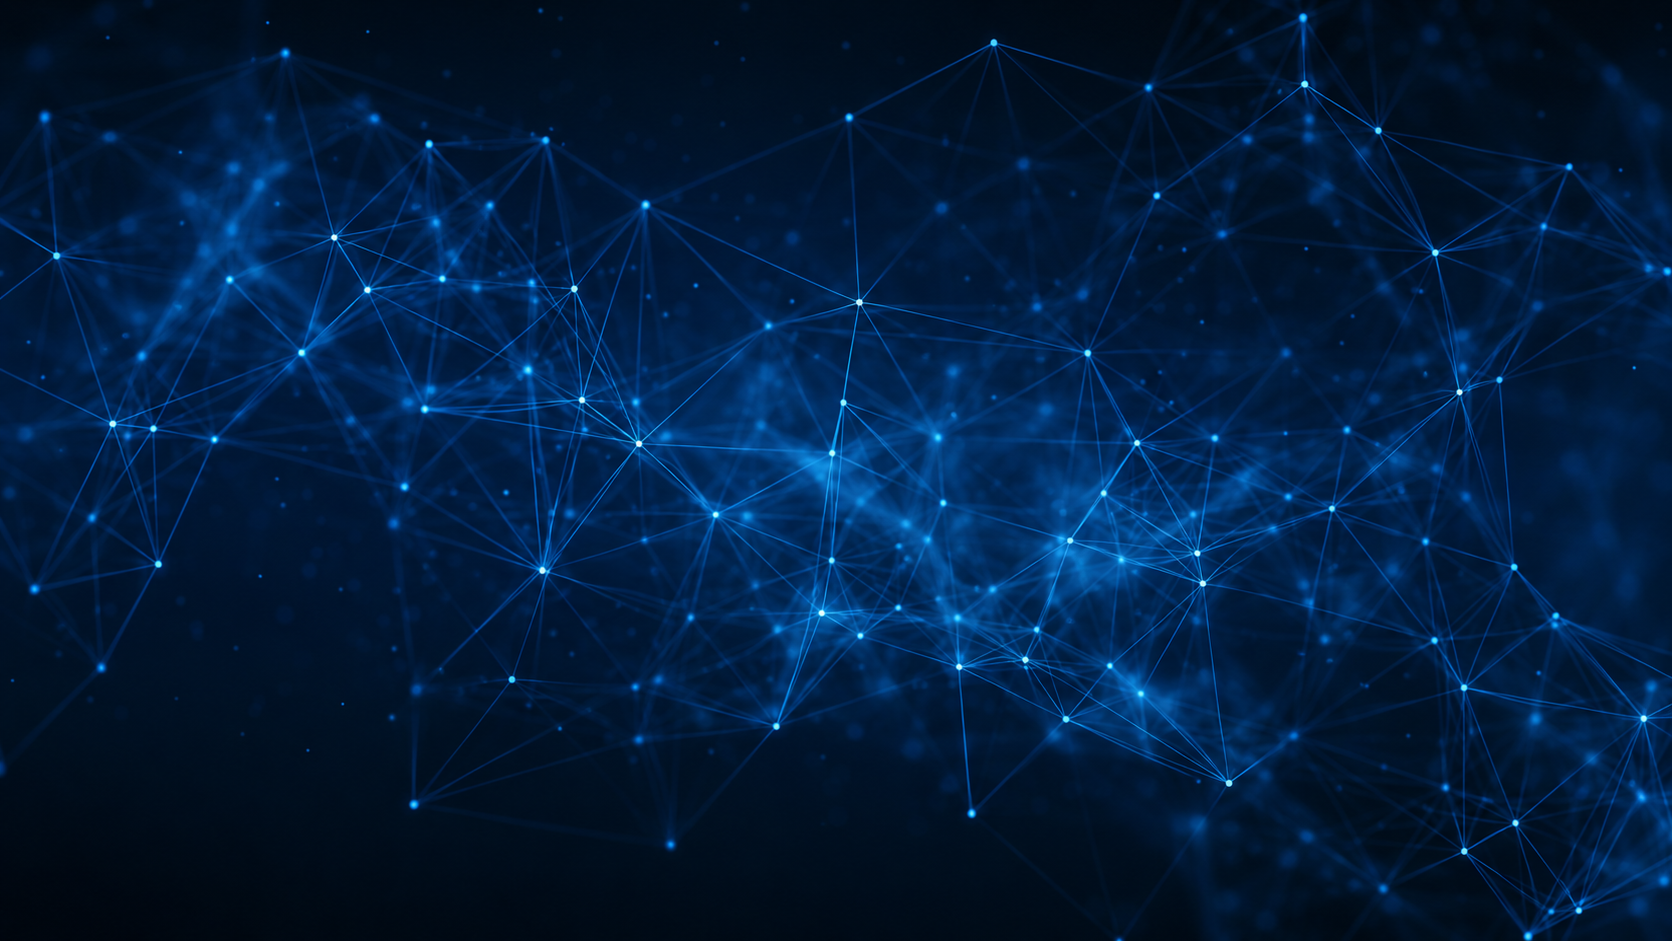
\includegraphics[width=\paperwidth, height=\paperheight]{121.png}
};
\fill[DarkBlue, opacity=0.72] (current page.south west) rectangle (current page.north east);

% Slide Number & Title
\node[anchor=west, text=TechYellow, font=\fontsize{14}{16}\selectfont\bfseries] at ([xshift=0.8cm,yshift=-0.65cm] current page.north west) {26};
\node[anchor=west, text=White, font=\fontsize{18}{22}\selectfont\bfseries] at ([xshift=1.8cm,yshift=-0.65cm] current page.north west) {References};

% Top Accent Divider Line
\draw[TechCyan, line width=0.8pt, opacity=0.6]
    ([xshift=0.8cm,yshift=-1.15cm] current page.north west) --
    ([xshift=15.2cm,yshift=-1.15cm] current page.north west);

% --------------------------------------------------
% REFERENCES LIST (UNBOXED ACADEMIC FORMAT)
% --------------------------------------------------

% Reference 1 (Slide 2)
\node[
    anchor=north west,
    text width=14.4cm,
    inner sep=0pt
]
at ([xshift=0.8cm,yshift=-1.35cm] current page.north west)
{
    \textcolor{TechYellow}{\fontsize{8.5}{11}\selectfont\bfseries [1]}\;\;\textcolor{White}{\fontsize{8}{10.5}\selectfont W. Shi, J. Cao, Q. Zhang, Y. Li, and L. Xu, ``Edge Computing: Vision and Challenges,'' \textit{IEEE Internet of Things Journal}, vol. 3, no. 5, pp. 637--646, 2016.}
};

% Reference 2 (Slide 5)
\node[
    anchor=north west,
    text width=14.4cm,
    inner sep=0pt
]
at ([xshift=0.8cm,yshift=-2.25cm] current page.north west)
{
    \textcolor{TechCyan}{\fontsize{8.5}{11}\selectfont\bfseries [2]}\;\;\textcolor{White}{\fontsize{8}{10.5}\selectfont L. F. Bittencourt et al., ``The Internet of Things, Fog and Cloud Continuum: Integration and Challenges,'' \textit{IEEE/ACM-related literature}, 2018.}
};

% Reference 3 (Slide 7)
\node[
    anchor=north west,
    text width=14.4cm,
    inner sep=0pt
]
at ([xshift=0.8cm,yshift=-3.15cm] current page.north west)
{
    \textcolor{TechYellow}{\fontsize{8.5}{11}\selectfont\bfseries [3]}\;\;\textcolor{White}{\fontsize{8}{10.5}\selectfont S. Hamdan, M. Ayyash, and S. Almajali, ``Edge-Computing Architectures for Internet of Things Applications: A Survey,'' \textit{Sensors}, vol. 20, no. 22, 6441, 2020.}
};

% Reference 4 (Slide 8)
\node[
    anchor=north west,
    text width=14.4cm,
    inner sep=0pt
]
at ([xshift=0.8cm,yshift=-4.15cm] current page.north west)
{
    \textcolor{TechCyan}{\fontsize{8.5}{11}\selectfont\bfseries [4]}\;\;\textcolor{White}{\fontsize{8}{10.5}\selectfont P. Gkonis, A. Giannopoulos, P. Trakadas, X. Masip-Bruin, and F. D'Andria, ``A Survey on IoT-Edge-Cloud Continuum Systems: Status, Challenges, Use Cases, and Open Issues,'' \textit{Future Internet}, vol. 15, no. 12, 383, 2023.}
};

% Reference 5 (Slide 11)
\node[
    anchor=north west,
    text width=14.4cm,
    inner sep=0pt
]
at ([xshift=0.8cm,yshift=-5.15cm] current page.north west)
{
    \textcolor{TechYellow}{\fontsize{8.5}{11}\selectfont\bfseries [5]}\;\;\textcolor{White}{\fontsize{8}{10.5}\selectfont Z. Zhou, X. Chen, E. Li, L. Zeng, K. Luo, and J. Zhang, ``Edge Intelligence: Paving the Last Mile of Artificial Intelligence With Edge Computing,'' \textit{Proceedings of the IEEE}, 2019.}
};

% Reference 6 (Slide 13)
\node[
    anchor=north west,
    text width=14.4cm,
    inner sep=0pt
]
at ([xshift=0.8cm,yshift=-6.15cm] current page.north west)
{
    \textcolor{TechCyan}{\fontsize{8.5}{11}\selectfont\bfseries [6]}\;\;\textcolor{White}{\fontsize{8}{10.5}\selectfont K. Cao et al., ``An Overview on Edge Computing Research,'' \textit{IEEE Access}, vol. 8, pp. 85714--85728, 2020.}
};

% Bottom Accent Line
\draw[TechCyan, line width=0.8pt, opacity=0.6]
    ([xshift=0.8cm,yshift=-7.05cm] current page.north west) --
    ([xshift=15.2cm,yshift=-7.05cm] current page.north west);

\end{tikzpicture}

\end{frame}

\end{document}